% =====================================================================
% ARBEITSFASSUNG (Kopie) – Fertigstellung der PA auf Branch pa-fertigstellung
% Diese Kopie wird von den To-dos (Umsetzungsplan_ToDos.md) geändert.
% Das Original unter PA/main.tex bleibt bis zum Abschluss unverändert.
% Pfade sind hier eine Ebene tiefer angepasst (../../ etc.).
% =====================================================================
\documentclass[12pt,a4paper]{article}

\usepackage[utf8]{inputenc}
\usepackage[T1]{fontenc}
\usepackage[ngerman]{babel}
\usepackage{lmodern}
\usepackage[a4paper,left=2.8cm,right=2.3cm,top=2.5cm,bottom=2.5cm]{geometry}
\usepackage{microtype}
\usepackage{graphicx}
\usepackage{booktabs}
\usepackage{tabularx}
\usepackage{longtable}
\usepackage{array}
\usepackage{enumitem}
\usepackage{amsmath}
\usepackage{xcolor}
\usepackage{float}
\usepackage{pdflscape}
\usepackage{fancyhdr}
\usepackage{xurl}
\usepackage{tikz}
\usetikzlibrary{arrows.meta,positioning,fit,backgrounds,shapes.geometric,calc}
% TikZ defines \path as a drawing command. Outside diagrams the report uses
% the same notation for breakable file paths; map it to url-style rendering.
\let\tikzpathcommand\path
\renewcommand{\path}[1]{\nolinkurl{#1}}
\usepackage[breaklinks=true]{hyperref}
\usepackage{csquotes}
\usepackage[backend=biber,style=authoryear,sorting=nyt]{biblatex}

% Vor Abgabe mit den offiziellen Angaben ersetzen.
\newcommand{\thwsAuthor}{Martin Rapps}
\newcommand{\thwsMatriculation}{6323014}
\newcommand{\thwsDegree}{B. Eng. Geovisualisierung}
\newcommand{\thwsFirstExaminer}{Dr. Markus Müller}
\newcommand{\thwsSecondExaminer}{Andreas Rupp}
\newcommand{\thwsSubmissionDate}{08.09.2026}

\addbibresource{references.bib}
% URLs in the bibliography are allowed to use a little extra stretch locally;
% this avoids suppressing useful line-break diagnostics in the main text.
\AtBeginBibliography{\sloppy}
\graphicspath{{../../}{../../figures/}{../../../docs/grafiken/verwendet_verbessert/}{../../../docs/grafiken/matrix_repeat_2026-08-17/}}
\hypersetup{colorlinks=true,linkcolor=blue,citecolor=blue,urlcolor=blue}
\setlist{itemsep=2pt,topsep=4pt}
\pagestyle{fancy}
\fancyhf{}
\fancyhead[L]{Projektarbeit -- Scan-to-BIM-Pipeline}
\fancyhead[R]{Studienbereich Geo}
\fancyfoot[C]{\thepage}
\setlength{\headheight}{15pt}

% Fuer eine kompakte PA koennen die optionalen Anhaenge hier deaktiviert werden.
\newif\ifincludeappendices
\includeappendicestrue

% Anonymisierte Fassung: via main_anonym.tex (\ANONYMVERSION)
\newif\ifanonym
\ifdefined\ANONYMVERSION\anonymtrue\else\anonymfalse\fi

\begin{document}
\pagenumbering{Roman}
\thispagestyle{empty}
\begin{center}
	{\large Technische Hochschule Würzburg-Schweinfurt\\
	Fakultät Kunststofftechnik und Vermessung\par}
	\vfill
	{\LARGE\bfseries Projektarbeit\par}
	\vspace{1.2cm}
	{\Large\bfseries KI-gestützte 3D-Rekonstruktion eines linearen Objekts\par}
	\vspace{0.4cm}
	{\large Konzeption, Robustheitsprüfung und geometrieerhaltende
	Meshgewinnung in einer Docker-basierten Scan-to-BIM-Pipeline\par}
	\vfill
	\begin{tabular}{@{}ll@{}}
		\ifanonym Studiengang: & \thwsDegree\\
		\else Vorgelegt von: & \thwsAuthor\\
		Matrikelnummer: & \thwsMatriculation\\
		Studiengang: & \thwsDegree\\
		\fi
		Erstprüfer/in: & \thwsFirstExaminer\\
		Zweitprüfer/in: & \thwsSecondExaminer\\
		Abgabetermin: & \thwsSubmissionDate
	\end{tabular}
	\vfill
	Würzburg, den \thwsSubmissionDate
\end{center}
\clearpage

\section*{Erklärung zur Projektarbeit}
Hiermit versichere ich, dass ich die vorliegende Arbeit eigenständig verfasst
und keine anderen als die angegebenen Quellen und Hilfsmittel verwendet habe.

Alle übernommenen Inhalte sowie mit Unterstützung von KI generierten Inhalte
wurden entsprechend den anerkannten wissenschaftlichen Grundsätzen oder
entsprechend der Regelungen zur Kennzeichnung von KI-Inhalten kenntlich
gemacht. Ausgenommen von der Kenntlichmachung sind orthografische oder
grammatikalische Korrekturen, Übersetzungen sowie nicht-sinnverändernde
Verbesserungen von Formulierungen. Ich bin mir bewusst, dass mit KI generierte
Texte keine Garantie für die Qualität von Inhalten und Text bieten. Daher
erkläre ich, dass ich KI-Werkzeuge lediglich als Hilfsmittel genutzt habe, die
von KI generierten Inhalte kritisch überprüft habe und mein eigenständiger
kognitiver sowie kreativer Einfluss in dieser Arbeit überwiegt. Ich versichere,
dass ich die Inhalte meiner Arbeit vollständig verstanden habe und
selbstständig vertreten kann.

Ich versichere, dass ich ausschließlich KI-Werkzeuge verwendet habe, deren
Nutzung vom Prüfer oder der Prüferin als Hilfsmittel zugelassen wurden.

\vfill
\noindent Würzburg, den \rule{4cm}{0.4pt}\hfill
\rule{6cm}{0.4pt}\\
\hfill Unterschrift des/der Studierenden
\clearpage
\ifanonym\else
\section*{Einwilligung zur Überprüfung einer Arbeit mit der
Plagiaterkennungssoftware PlagAware}

\vspace{0.5em}
\noindent\begin{tabular}{@{}p{2.2cm}p{4.4cm}p{1.8cm}l@{}}
Name: & Rapps & Vorname: & Martin\\[0.4em]
Matr.Nr.: & 6323014 & & \\[0.4em]
Adresse: & \dotfill & & \\[0.4em]
eMail: & \dotfill & Studiengang: & B.\,Eng.\ Geovisualisierung\\
\end{tabular}

\vspace{0.4em}
\noindent\begin{tabular}{@{}p{2.2cm}p{10.8cm}@{}}
Titel der Arbeit: & KI-gestützte 3D-Rekonstruktion eines linearen Objekts --
Konzeption, Robustheitsprüfung und geometrieerhaltende Meshgewinnung in einer
Docker-basierten Scan-to-BIM-Pipeline\\
\end{tabular}

\vspace{0.8em}
Die THWS überprüft Prüfungsarbeiten (Studien-, Projekt-, Bachelor- und
Masterarbeiten) mit Hilfe der Plagiaterkennungssoftware PlagAware. Die zu
überprüfenden Arbeiten werden an den Dienst der Software übermittelt, dort auf
Übereinstimmung mit externen Quellen untersucht und zum Zwecke des Abgleichs
mit zukünftig zu überprüfenden Arbeiten gespeichert. Die befristete Speicherung
der Arbeit in der Datenbank sowie die Weitergabe der persönlichen Daten im
Rahmen der Plagiatsprüfung ist nur mit Einwilligung zulässig.

\vspace{0.4em}
\noindent\fbox{\parbox{\dimexpr\textwidth-2\fboxsep-2\fboxrule\relax}{Mit der
Unterschrift erkläre ich meine Einwilligung, dass
\begin{itemize}[leftmargin=1.4em,itemsep=2pt]
  \item die von mir vorgelegte und verfasste Arbeit zum Zwecke der Überprüfung
        auf Plagiate hin an PlagAware übermittelt und vorübergehend (5~Jahre)
        in der von PlagAware geführten Datenbank gespeichert wird;
  \item meine persönlichen Daten (Vorname, Name, studentische eMail-Adresse)
        zusammen mit dem Text digital gespeichert und verwendet werden. Diese
        Daten sind nur meinen Prüferinnen und/oder Prüfern zugänglich.
\end{itemize}}}

\vfill
\noindent Ort, Datum: \dotfill\hfill Unterschrift: \dotfill
\fi
\section*{Kurzfassung}
Diese Projektarbeit untersucht die Machbarkeit einer Docker-basierten Pipeline zur
objektbezogenen Rekonstruktion eines linearen Testobjekts. Der Workflow verbindet
SAM~3.1 für die temporale 2D-Segmentierung, COLMAP für die Kamerageometrie,
Segment-then-Splat für objektspezifische 3D-Gaussians, SuGaR beziehungsweise eine
geometrieerhaltende Original-GS-Meshroute und DGtal für die Centerline-Extraktion.
Für den Testdatensatz ist die Kette vollständig nachgewiesen: 240 von 240 Bildern
wurden registriert; alle zwölf SuGaR-Coarse-Folgeläufe, neun erfolgreiche Autopilot-Volläufe
und der Qualitätsvergleichsbatch ohne Fehlerfall sind mit Manifeststatus
\texttt{success} archiviert. Für die
Produktionskonfiguration (OPENCV, 5~FPS, 720p, Route A) werden 29,62\,dB
objektmaskierte PSNR erreicht; die Nachweise stammen aus archivierten Matrix-,
Replay- und Autopilotläufen. Der Schwerpunkt liegt auf der technischen
Funktionsfähigkeit, der sauberen Trennung von Bilddomänen und der reproduzierbaren
Auswertung. Die Arbeit ist ein Machbarkeitsnachweis für die spätere
Bachelorarbeit; ein geodätischer Genauigkeitsnachweis für reale Rohr- oder
Kabeltrassen ist nicht Gegenstand.
\clearpage

\tableofcontents
\listoffigures
\listoftables
\clearpage
\pagenumbering{arabic}

\section{Einleitung}

\subsection{Motivation und Problemstellung}

Die Rekonstruktion dünner, linearer Objekte aus Bildsequenzen verbindet mehrere
schwierige Teilprobleme: Die Kamerabewegung muss stabil geschätzt werden, das
Objekt muss über die Bilder hinweg konsistent segmentiert werden und die
objektbezogene 3D-Repräsentation muss für nachgelagerte Geometrieoperationen
verwendbar sein. Die Projektarbeit untersucht diesen Ablauf zunächst an einem
kontrollierten Alurohr-Testdatensatz. Die spätere Bachelorarbeit soll die
Pipeline auf reale Rohr- oder Kabeltrassen und geodätische Referenzen
übertragen.

\subsection{Zielsetzung und Eigenbeitrag}

Das Ziel der Projektarbeit ist ein technischer Machbarkeitsnachweis. Dazu muss
die Pipeline vom Video bis zur lokalen Centerline durchlaufen, die zentralen
Datenverträge müssen überprüfbar sein und die wichtigsten Varianten müssen mit
reproduzierbaren Parametern verglichen werden. Eine Aussage über die Einhaltung
einer Toleranz von \(\pm 10\,\mathrm{cm}\) wird für die Projektarbeit nicht
behauptet, weil dafür noch geeignete GNSS- oder Vermessungsreferenzen fehlen.
Der Eigenbeitrag liegt in der Integration der heterogenen Komponenten, der
Trennung von Roh- und Idealbilddomäne (die verzeichnungsbehafteten Rohbilder
werden in verzeichnungsfreie PINHOLE-Bilder überführt, sodass Masken,
Kamerageometrie, Splatting und Auswertung in derselben, konsistenten Domäne
arbeiten), der Definition überprüfbarer Datenverträge (Schnittstellenregeln,
die festlegen, welche Artefakte in welcher Bilddomäne zueinander passen
müssen und nach welchen Kriterien eine Stufe als gültig gilt), der
maskengetriebenen Objekt- und Meshgewinnung sowie der automatisierten
Durchführung und wissenschaftlichen Interpretation der Tests. STS und SuGaR
sind dabei genutzte, nicht selbst entworfene Verfahren; der eigene Anteil in
der Segmentierung liegt in der angepassten Maskenlogik: die Erosionshierarchie
(default unverändert, middle und small erodiert) sowie die promptbasierte
Auswahl sorgen dafür, dass automatisch genau ein
segmentiertes Zielobjekt entsteht. Das offizielle STS-Verfahren geht davon
verschieden, indem es sämtliche Szenenobjekte automatisch in drei
Granularitätsstufen erfasst und erst nach der Rekonstruktion eine offene
Textabfrage ermöglicht; der Objektprompt legt das Ziel hier dagegen bereits
vor dem Training fest, sodass Mehrfachsegmentierung und Nachabfrage
entfallen. Die Funktionsweise ist in
Abschnitt~\ref{sec:grundlagen} beschrieben.
Der Einsatz von SAM~3.1 verdoppelt zudem die Verarbeitungsgeschwindigkeit für
Videos mit mittlerer Objektanzahl (16 auf 32 Frames pro Sekunde auf einer
einzelnen H100-GPU) \parencite{metaSam3}.

\subsection{Forschungsfragen}

Die zentrale Arbeitsfrage lautet:
\begin{quote}
Lässt sich eine Docker-orchestrierte, objektbezogene Scan-to-BIM-Pipeline aus
promptbarer SAM-3.1-Segmentierung, kameramodellbewusstem COLMAP-SfM,
Segment-then-Splat und meshbasierter Nachverarbeitung für ein lineares
Testobjekt robust und reproduzierbar bis zu einer lokalen Centerline betreiben?
\end{quote}

Zur Beantwortung werden vier Unterfragen betrachtet:

\begin{enumerate}
  \item Welche Bilddomänen, Datenverträge und Quality-Gates sind erforderlich,
	  damit Masken, Kameras, Eval-Split, Gaussians, Mesh und Centerline
	  konsistent übergeben werden?
  \item Wie beeinflussen Kameramodell, zeitliche Abtastung und Bildauflösung
	  den technischen Pipelineerfolg und die objektmaskierten Bildmetriken?
  \item Welche der untersuchten Meshrouten -- direkte Original-STS-GS-Route A
	  oder SuGaR-Coarse -- bewahrt die für die Centerline benötigte
	  Objektgeometrie im Projektstand geeigneter?
  \item Inwieweit ermöglichen interaktiver CLI-Betrieb, Replay, Autopilot und
	  Matrixrunner reproduzierbare Einzel- und Batchläufe?
\end{enumerate}

\subsection{Abgrenzung und Aufbau}

Die Arbeit konzentriert sich auf Grundlagen, Konzept, Implementierung,
Funktions- und Vergleichstests sowie die Interpretation der Ergebnisse. Lange
Installationsanleitungen, vollständige Quellcode-Dokumentation und spätere
Bachelorarbeitsfragen werden bewusst außerhalb des Haupttextes gehalten. Nicht
Gegenstand sind eine reale Vermessung einer Kabeltrasse, ein Nachweis von
$\pm10\,\mathrm{cm}$, eine vollständige Bewertung aller Kameramodelle, eine
allgemeine Einführung in Computer Vision oder eine Produktionsentscheidung
allein aus PSNR, SSIM und LPIPS. Die vorhandene Web-UI bleibt ebenfalls
außerhalb des Untersuchungsumfangs und ist der späteren Bachelorarbeit
vorbehalten; betrachtet werden CLI, Autopilot, Replay
und Matrixrunner.

\section{Datengrundlage und Anwendungsrahmen}
\label{sec:datengrundlage}

\subsection{Alurohr als kontrollierter Testdatensatz}

Die Projektarbeit verwendet eine etwa 48 Sekunden lange Videosequenz eines
Alurohrs als kontrollierten Labordatensatz. Das Rohr repräsentiert ein dünnes,
lineares Objekt, dessen Bildfläche sich mit Kameraposition, Blickwinkel und
Auflösung deutlich verändert. Der Datensatz dient nicht als maßstäblicher
Ersatz für ein im Baugraben liegendes Kabel. Er ermöglicht jedoch, die
Datenübergaben und Fehlerfälle einer vollständigen Rekonstruktionskette unter
wiederholbaren Bedingungen zu untersuchen.

\subsection{Aufnahmekamera und Videoeinstellungen}

Die Videosequenz wurde durchgehend mit der Hauptkamera (1x-Weitwinkelkamera)
des Google Pixel 8 Pro aufgenommen. Diese Kamera besitzt laut
Herstellerangaben einen 50-MP-Sensor mit einer Blende von $f/1{,}68$, einem
Sichtfeld von etwa $82^\circ$ und einer Sensorgröße von $1/1{,}31$ Zoll;
Google weist für die Weitwinkelkamera außerdem optische und elektronische
Bildstabilisierung aus \parencite{googlePixel8ProSpecs}. Die Aufnahme erfolgte
mit der OpenCamera-App. OpenCamera unterstützt eine Belichtungssperre sowie
die Auswahl der Videoauflösung; die automatische Bildausrichtung (Auto-Level)
ist eine separate, optionale Funktion \parencite{openCameraHelp}.

Für den verwendeten Datensatz waren die Belichtung fest eingestellt, die
Auflösung auf $1920\times1080$ Pixel (Full HD) gesetzt und die automatische
Bildlagenkorrektur beziehungsweise nachträgliche Bildausrichtung deaktiviert.
Die Rohdatei \path{data/01_raw/Alurohr_THWS.mp4} ist ein H.264-Video mit
$1920\times1080$ Pixeln, nominal 30 FPS, 1441 Bildern und einer Dauer von rund
48 Sekunden. Die späteren 5- beziehungsweise 2-FPS-
Profile sowie die Zielauflösungen 720p, qHD und Low sind daraus abgeleitete
Pipeline-Arbeitsprofile und keine zusätzlichen Kameraaufnahmen.

Die Bezeichnung ``unverfälschtes Video'' ist dabei auf die fehlende zusätzliche
App-seitige Bildausrichtung und die festgehaltene Belichtung zu beziehen. Die
Aufnahme ist kein Rohsensordatensatz: Das Pixel verarbeitet das Signal bereits
über seine interne Bildverarbeitung und speichert hier ein H.264-Video.
Insbesondere lässt sich aus der Datei allein nicht sicher nachweisen, ob die
vom Gerät bereitgestellte optische beziehungsweise elektronische
Videostabilisierung vollständig deaktiviert war. Die PA behauptet daher keine
vollständig unverarbeitete Sensoraufnahme, sondern dokumentiert ein unter
festgelegten Aufnahmeparametern erzeugtes Rohvideo für die nachgelagerte
Pipeline.

Der Segmentierungsprompt lautet \texttt{pipe}. Die in der Projektarbeit
untersuchten Profilvarianten aus zwei zeitlichen Abtastungen (2 und 5 FPS) und
drei räumlichen Auflösungen ($1280\times720$, $960\times540$ und
$640\times360$ Pixel) sind in Kapitel~\ref{sec:versuchsaufbau} zusammengefasst;
für den Datensatz genügt hier der Hinweis, dass ein Lauf bei 5 FPS rund 240
Frames und bei 2 FPS rund 96 Frames umfasst. Ein Lauf verwendet in allen
Verarbeitungsstufen denselben Frame-Satz, sodass Bildnamen, Masken, Kameras
und feste Evaluationsansichten innerhalb eines Laufs konsistent bleiben.

\subsection{Scope des linearen Einobjektfalls}

Die Centerline-Nachverarbeitung ist bewusst auf ein einzelnes lineares Objekt
begrenzt. Verzweigte Leitungsnetze erfordern eine zusätzliche Trennung echter
Abzweigungen von Skelettartefakten. Gerade auf dünnwandigen und verrauschten
Meshes kann die Skelettierung Medialflächen\footnote{Medialflächen sind
zweidimensionale, flächige Skelettbereiche: Sie entstehen, wenn von einem
inneren Punkt mehrere Punkte der Objektoberfläche gleich weit entfernt sind
(zum Beispiel bei flachen oder dünnwandigen Strukturen). Für eine
Linientrasse sind sie nicht direkt verwertbar und müssen auf ihren
Durchmesserpfad reduziert werden.\label{fn:medialflaechen}} und zahlreiche
kurze Stachel-Äste erzeugen. Der produktive \texttt{single}-Modus reduziert
deshalb die größte zusammenhängende Skelettkomponente auf ihren
Durchmesserpfad.

Das primäre analytische Produkt der PA ist die lokale Centerline. Masken,
COLMAP-Modell, STS-Gaussians und Mesh sind notwendige und diagnostisch wichtige
Zwischenprodukte. CSV-, B-Spline- und GeoJSON-Dateien werden ebenfalls erzeugt,
aber wegen der noch fehlenden unabhängigen Transformations- und
Vermessungsreferenz nicht als global genaue Endprodukte bewertet.

\subsection{Referenzlage und Aussagegrenzen}

Für den aktuellen Testdatensatz liegt keine unabhängig eingemessene
GNSS-Referenzkurve vor. Vorhandene GCP-Dateien bilden nur einen synthetischen
beziehungsweise lokalen Test der Dateiverträge. Fehlt eine validierte
4x4-Ähnlichkeitstransformation, kann die Pipeline einen explizit bezeichneten
Translation-Fallback ausführen. Dieser prüft den Exportpfad, aber weder Rotation
und Maßstab noch Lage- und Höhengenauigkeit.

Daraus folgt die zentrale Abgrenzung: Die PA bewertet Funktionsfähigkeit,
Robustheit, Reproduzierbarkeit, objektmaskierte Ansichtsqualität und relative
Unterschiede zwischen Meshrouten. Ein Nachweis der später angestrebten
Toleranz von $\pm10\,\mathrm{cm}$ ist erst mit realen GCP-/GNSS-Messungen,
einer validierten Transformation und geometrischen Vergleichsmetriken möglich.

\section{Technische und methodische Grundlagen}
\label{sec:grundlagen}

Dieses Kapitel führt die Verfahren ein, die für Architektur,
Versuchsdesign und Interpretation der Pipeline notwendig sind. Die Arbeit
entwickelt keine neuen Segmentierungs-, SfM- oder Splatting-Algorithmen. Ihre
wissenschaftliche Leistung liegt in der konsistenten Verbindung und Prüfung
dieser Verfahren.

\subsection{Promptbare temporale Segmentierung}

Das Segment Anything Model überführt visuelle beziehungsweise sprachliche
Prompts in Objektmasken \parencite{kirillov2023segment,metaSam3}. Für die
Pipeline ist die Promptbarkeit wichtig. Die Zielklasse kann als Begriff wie
\texttt{pipe} angegeben werden, ohne für jede neue lineare Objektart ein
eigenes Modell zu trainieren. Die Videoverarbeitung propagiert die
Objektdefinition über die Sequenz. Damit wird die zeitliche Konsistenz der
Masken zu einem eigenen Qualitätskriterium. Eine gute Einzelbildmaske genügt
nicht, wenn das Objekt in späteren Frames verloren geht.

Der kanonische SAM-Ausgang wird als Hierarchie gespeichert. \texttt{default}
ist die unveränderte Objektmaske, \texttt{middle} entsteht durch eine
$5\times5$-Erosion und \texttt{small} durch zwei Erosionsschritte. Die
Erosion wendet ein quadratisches Strukturelement von $5\times5$ Pixeln an:
Ein Pixel gehört nur dann weiterhin zur Maske, wenn die gesamte
$5\times5$-Nachbarschaft maskiert ist. Dadurch werden unsichere Randpixel
rund zwei Pixel breit entfernt. Der Wert $5\times5$ ist ein pragmatischer
Standard. Er glättet unscharfe Maskenränder und entfernt dünne
Rauschfragmente, ohne das dünne lineare Objekt über eine sinnvolle Bildbreite
hinaus schrumpfen zu lassen. Die konservativeren Stufen entfernen zusätzlich
unsichere Randpixel, können bei sehr dünnen Objekten aber auch relevante
Objektfläche verlieren. Maskenstufe und optionale Dilatation sind deshalb
explizite Parameter. In der aktuellen Projektfassung wird keine Dilatation
angewendet. Historisch war zwischenzeitlich auch die \texttt{default}-Maske
dilatiert. Solche Stände werden als Entwicklungszwischenstände nicht
fortgeführt, sondern durch die verbindliche Festlegung
\texttt{default} = unverändert, \texttt{middle} = einfach erodiert und
\texttt{small} = zweifach erodiert ersetzt (vgl. Abschnitt~\ref{sec:versuchsaufbau}).

\subsection{Structure-from-Motion und Kameramodelle}

Structure-from-Motion schätzt aus korrespondierenden Bildmerkmalen die
Kameraposen und eine sparse 3D-Punktwolke. COLMAP verbindet dafür
SIFT-Merkmalsextraktion, Matching, inkrementelles Mapping und Bundle Adjustment
\parencite{schoenberger2016sfm}. Die Pipeline verwendet unmaskierte Bilder:
Hintergrund- und Ankermerkmale stabilisieren die Orientierung eines glatten,
dünnen Zielobjekts und bleiben für einen späteren GCP-Bezug verfügbar.

Für die Projektarbeit sind drei Kameramodelle relevant. \texttt{PINHOLE}
modelliert getrennte Brennweiten und einen Hauptpunkt, aber keine Verzeichnung. Es setzt damit eine
ideale Bilddomäne voraus. \texttt{SIMPLE\_RADIAL} ergänzt eine gemeinsame
Brennweite um einen radialen Verzeichnungsparameter. \texttt{OPENCV} besitzt
zusätzliche radiale und tangentiale Freiheitsgrade. Das flexiblere Modell ist
nicht grundsätzlich überlegen, da zusätzliche Freiheitsgrade eine
flächendeckende und rauschfreie Merkmalsverteilung voraussetzen. Fehlt diese,
ist das Gleichungssystem schlecht konditioniert – der Optimierer neigt dann
zum Overfitting auf Bildrauschen oder koppelt Verzeichnungsparameter
fälschlicherweise an Kamerabewegungen. Als Produktionsstandard
ist \texttt{OPENCV} gewählt. Die Begründung aus der Matrixauswertung steht in
Abschnitt~\ref{sec:produktionskonfiguration}.

Die Modellbezeichnung ist dabei keine hinterlegte Objektivkalibrierung. Das
Skript \texttt{run\_sfm.sh} übergibt COLMAP lediglich die Modellfamilie und mit
\mbox{\path{ImageReader.single_camera=1}} die Annahme eines gemeinsamen
Kameramodells für alle Frames eines Laufs. Eine externe
\texttt{camera\_params}-Datei oder eine Checkerboard-Kalibrierung wird nicht
eingelesen. COLMAP initialisiert die Parameter intern und schätzt Brennweiten,
Hauptpunkt und Verzeichnungskoeffizienten anschließend gemeinsam mit
Kameraposen und 3D-Punkten aus den Bildkorrespondenzen. Die Werte in
\texttt{sparse\_txt/cameras.txt} sind daher lauf- und auflösungsabhängige
Schätzwerte, keine allgemeinen Standarddaten der Kamera.

Bei verzeichnungsbehafteten Modellen bleibt das geschätzte Originalmodell für
SfM und GCP erhalten. Anschließend erzeugt der COLMAP-
\texttt{image\_undistorter} eine ideale PINHOLE-Szene für STS und die
Meshroute. Bei PINHOLE-Eingaben wird am selben Schnittstellenpfad eine
unveränderte Pass-through-Szene bereitgestellt. Diese Unterscheidung ist
entscheidend: Ein direkter PINHOLE-Lauf auf Rohbildern ist eine Ablation der
Modellannahme und kein Nachweis einer erfolgreichen Entzerrung.

\subsection{3D Gaussian Splatting und Segment-then-Splat}

3D Gaussian Splatting stellt eine Szene als Menge anisotroper Gaussians dar
\parencite{kerbl2023gaussian}, das heißt als Ansammlung kleiner, elliptischer
3D-Verteilungen, deren Form und räumliche Ausrichtung pro Gaussian frei
gelernt werden. Ein Gaussian $i$ besitzt unter anderem einen
Mittelpunkt $\boldsymbol{\mu}_i$, eine räumliche Kovarianz
$\boldsymbol{\Sigma}_i$, Opazität $\alpha_i$ und blickabhängige Farbe. Eine
übliche Zerlegung der Kovarianz lautet

\begin{equation}
	\boldsymbol{\Sigma}_i =
	\mathbf{R}_i\,\mathbf{S}_i\mathbf{S}_i^{\top}\mathbf{R}_i^{\top},
	\label{eq:gaussian-covariance}
\end{equation}

wobei $\mathbf{R}_i$ die Orientierung und $\mathbf{S}_i$ die Skalierung
beschreibt. Beim Rendering werden die Gaussians in die Kamera projiziert,
sortiert und über Alpha-Compositing zu einem Bild zusammengeführt. Die
Repräsentation ist deshalb zugleich geometrische Hypothese und renderbare
Radiance-Field-Darstellung.

Segment-then-Splat ergänzt die Gaussians um objektbezogene Zuordnungen
\parencite{lu2025segment}. Das offizielle Verfahren gewinnt seine
Mehrfachansichtsmasken über eine SAM-basierte Tracking-Pipeline
(AutoSeg-SAM2). Ein SAM-Grid-Prompt segmentiert die erste Ansicht, SAM~2
verfolgt das Objekt anschließend über die Sequenz. Nach der Rekonstruktion
wird jedem Objekt ein CLIP-Embedding zugeordnet, über das die Szene offen
vokabularisch durchsucht werden kann. In der Projektpipeline übernehmen die
extern erzeugten SAM-3.1-Masken beide Rollen. Die promptbare temporale
Segmentierung liefert die Objektmasken direkt, und die CLIP-Embedding-
Zuordnung entfällt, weil für den linearen Einobjektfall ausschließlich die
gewählte Objektmaske als Suchbegriff benötigt wird. STS initialisiert die
Szene aus dem COLMAP-Modell und ordnet jeden Gaussian über die vorgegebenen
Masken einem Objekt zu. Während der Objekt-/Maskenphase wird der Bildverlust
auf die maskierte Objektregion der zugeordneten Maske begrenzt, eine
anschließende All-Object-Phase optimiert alle Objekte gemeinsam. In der
Projektpipeline sind diese Masken die bereits segmentierten Eingabebilder in
den drei Erosionsstufen (\texttt{default}, \texttt{middle}, \texttt{small}),
nicht eine vom STS-System erzeugte Nachsegmentierung. Der Projektstandard
umfasst 7.000 Gesamtiterationen, aufgeteilt in 5.000 Iterationen des
Objektcurriculums und 2.000 Iterationen der All-Object-Phase. Da im vorliegenden
Einobjekt-Szenario keine weiteren Instanzen existieren, bewirkt die finale
Phase keine zusätzliche semantische Entflechtung, sondern dient als konsistente
Trainingsfortführung des isolierten Zielobjekts.

Die Maskenstufen entfalten ihre Wirkung dabei je Komponente getrennt: STS
setzt die bereitgestellten Masken für die Objektzuordnung und die
Objektphasen-Supervision ein. Darüber hinaus ist \texttt{middle} aktuell
allein in der Coverage-Prüfung sowie der Kamera- und Eval-Split-Auswahl
wirksam — Ansichten mit leerer \texttt{middle}-Maske werden vom STS-Training
beziehungsweise von der Evaluation ausgeschlossen. Unabhängig davon belegen
die historischen Zwischenstände in Abbildung~\ref{fig:pa-panel-mesh}, dass
die \texttt{middle}-Stufe die Objektabgrenzung visuell stabilisiert. Der
gezielte Einsatz unterschiedlicher Maskenstufen in den Verlustpfaden der
SuGaR-Vergleichsroute gehört zum maskenbewussten SuGaR-Fork und wird deshalb
zusammen mit diesem Verfahren in Abschnitt~\ref{subsec:meshgewinnung}
beschrieben.

\subsection{Objektselektion und Meshgewinnung}
\label{subsec:meshgewinnung}

Die Ziel-Gaussians werden über die konfigurierte Objekt-ID selektiert. Bei einem
Datensatz mit genau einem linearen Objekt ist die Objekt-ID eine
Formalschnittstelle des übernommenen STS-Schemas. Die eigentliche Auswahl
trifft der nachgelagerte Opazitäts- und Farbfilter. Ein Opazitätsfilter kann
schwach sichtbare Primitive entfernen. Die in der PLY gespeicherte
Logit-Opazität $o_i$ ist der rohe, unbeschränkte Voraktivierungswert, den das
3DGS-Modell lernt. Sie wird erst durch die Sigmoid-Funktion

\begin{equation}
	\alpha_i = \frac{1}{1+\exp(-o_i)}
	\label{eq:opacity}
\end{equation}

in die sichtbare Alpha-Opazität im Bereich $[0,1]$ überführt. Das Filtern über
den Logit erlaubt dabei einen gleichmäßigeren Zugriff auf kleine
Transparenzwerte, als die bereits gesättigte Alpha-Kurve anbieten würde. Nach
Objekt-, Opazitäts- und optionaler Farbauswahl erzeugt die Pipeline eine
getrennte Hochopazitätskopie. Das Setzen auf $\alpha=0{,}999999$ ist eine
Initialisierungspolitik für die geometrische Extraktion, keine physikalische
Aussage über Materialtransparenz: Ein endlicher Wert von exakt 1 ist nach der
Sigmoid-Aktivierung numerisch nicht erreichbar, weil er einen unendlichen
Logit erfordern würde. Der nahezu opake Wert stabilisiert die anschließende
Dichte- und Normalenberechnung beim Surface-Sampling.

SuGaR richtet in seiner vollständigen Route 3D-Gaussians durch
Oberflächenregularisierung als flache Strukturen an einer Oberfläche aus und
rekonstruiert daraus über kamerabasierte Stichproben ein
Poisson-Mesh\footnote{Die Poisson-Oberflächenrekonstruktion legt durch eine
Punktwolke mit orientierten Normalen eine glatte Oberfläche, indem sie ein
Poisson-Gleichungssystem löst, dessen Lösungsfeld die gesuchte
Indikatorfunktion der Oberfläche beschreibt \parencite{kazhdan2006poisson}.}
\parencite{guedon2024sugar}. Im Standardverfahren vergleicht SuGaR stets das
gesamte gerenderte Bild mit dem Trainingsfoto. Da für die Rohrrekonstruktion
jedoch ausschließlich das freigestellte Zielobjekt optimiert werden soll,
begrenzt der im Rahmen dieser Arbeit angepasste lokale SuGaR-Fork den
photometrischen Optimierungsverlust gezielt auf die 2D-Objektmaske:

\begin{equation}
	\mathcal{L}_{\mathrm{RGB}}^{M} =
	\frac{\sum_p M(p)\,\ell_{\mathrm{RGB}}(p)}
	{\sum_p M(p) + \varepsilon}.
	\label{eq:masked-rgb-loss}
\end{equation}

Hierbei ist $M(p) \in \{0, 1\}$ die binäre Objektmaske an Pixelposition $p$
(1 auf dem Rohr, 0 im Hintergrund) und $\ell_{\mathrm{RGB}}(p)$ der kombinierte
Farb- und Strukturfehler ($L_1$-Distanz und DSSIM). Durch die Multiplikation
mit $M(p)$ wird der Fehler im Hintergrund zu null gesetzt, sodass der
Optimierer ausschließlich Gradienten für die Gaussians des Zielobjekts
berechnet und den Hintergrund ignoriert. Die Division durch die Summe aller
Maskenpixel $\sum_p M(p)$ normiert den Verlust auf den Mittelwert pro
Objektpixel. Die winzige Konstante $\varepsilon = 10^{-7}$ schützt vor einer
Division durch null bei temporär leeren Masken.

Beide maskennutzenden Verlustpfade des maskenbewussten SuGaR-Coarse-Trainings
verwenden unterschiedliche Maskenstufen. Die RGB-Supervision nach
Gl.~\ref{eq:masked-rgb-loss} vergleicht das Splat-Rendering jeder
Trainingskamera pixelweise mit dem aufgenommenen Bild, begrenzt auf die
Maskenpixel (maskierter L1-Anteil plus maskierter DSSIM-Anteil mit einem
$11\times11$-Fenster. Das lokale Fenster zieht am Maskenrand begrenzt Kontext
von außen ein). Sie verwendet die unveränderte \texttt{default}-Maske, damit
die Bildsupervision möglichst die volle Objektprojektion abdeckt und
Positionen, Opazitäten und Farben der Objekt-Gaussians vollständig
spezifiziert werden. Eine Farbprojektion auf eine Oberfläche findet dabei
nicht statt. Die Farbübertragung aus den Ansichten erfolgt erst in der
nachgelagerten UV-Texturphase des Forks.

Die Depth-Normal-Consistency (DN) vergleicht dagegen die aus der gerenderten
Gaussian-Tiefe abgeleiteten Normalen mit den gerenderten Normalen und wird
bewusst auf der erodierten \texttt{middle}-Stufe ohne Dilatation angewandt.
Der Grund ist die Silhouettenstabilität. Tiefe und daraus abgeleitete Normalen
sind direkt an Objektkanten unzuverlässig und genau dort kann eine
\texttt{default}-Maske über die Objektsilhouette hinausragen. Ein solcher
Maskenüberhang würde die Objektnormalen am Silhouettenrand in Richtung der
Hintergrundtiefe ziehen und dadurch eine ausgestülpte oder abgeflachte
Oberfläche erzeugen. \texttt{middle} entfernt diese unsichere Randzone von
rund zwei Pixeln, sodass nur Pixel supervisiert werden, die sicher auf dem
Objekt liegen.

Diese Aufteilung stammt aus der Entwicklung des Forks und ist dort Teil des
Datenvertrags zwischen Maskenhierarchie und Trainingsplan. Da die
DN-/SDF-Terme erst oberhalb des Zählerstands 9.000 aktiviert werden und alle
ausgewerteten Läufe — einschließlich sämtlicher \texttt{sugar\_coarse}-Arme
der Vierfeld-Ablation und der Folgeprüfung — mit Zielzählerstand 9.000 oder
weniger trainiert wurden, trat der DN-Term in keinem ausgewerteten Lauf
tatsächlich in Wirkung. Die \texttt{middle}-Zuordnung bleibt dennoch
dokumentiert, weil sie den Fork-Vertrag definiert. Zählermechanik und
Nachweislage der Läufe sind in Abschnitt~\ref{subsec:sugar-folgepruefung}
erläutert. Standardläufe mit Zieliteration 9.000 optimieren die Geometrie
daher primär über den maskierten photometrischen Farbverlust.


Auf dieser Basis definiert das Projekt eine direkte Meshroute, die ohne
Coarse-Training auskommt: Sie überspringt die zusätzliche SuGaR-Coarse-
Optimierung, das Gaussian-bound Refinement und das UV-Baking. Sie verwendet
Original-STS-Gaussians mit projizierter Diamond-Mesh-Tiefe\footnote{Die
Diamond-Mesh-Tiefe wird aus der Projektion der SuGaR-``Diamond''-Primitive
gewonnen: Diese flachen, an den Gaussians ausgerichteten Vierecksflächen
werden in einen Z-Buffer projiziert, aus dem je Pixel eine Tiefe abgelesen
wird; das Surface-Sampling wandelt diese Tiefe anschließend in 3D-Punkte. Die
Alternative ist die Tiefe direkt aus dem Gaussian-Rasterizer.}, Surface-
Sampling, Poisson-Rekonstruktion, Dichtebereinigung, Decimation und optionale
Vertexprojektion. Die Dichtebereinigung entfernt Cluster mit zu wenigen
Stützpunkten, die Decimation reduziert die Dreieckszahl auf das Ziel-Vertice-
Budget, und die optionale Vertexprojektion verschiebt die verbliebenen
Vertices auf die nächstgelegenen Oberflächenstichproben beziehungsweise deren
Tiefenpunkte. Diese Konfiguration entspricht genau der Zelle A der
kontrollierten Vierfeld-Ablation (Abschnitt~\ref{subsec:vierfeld-ablation});
nach dieser Zelle wird sie im Folgenden durchgängig als \emph{Route A}
bezeichnet, während die Coarse-Route entsprechend dem Modusnamen des
Ausführungscodes \texttt{sugar\_coarse} heißt; Route A selbst trägt dort den
Modusnamen \texttt{original\_gs}. Die vollständige SuGaR-Coarse-Route bleibt als
wissenschaftlicher Vergleich erhalten. Damit werden zwei Fragen getrennt:
Wie wird aus einer Gaussian-Wolke ein Mesh gewonnen, und wie verändert eine
zusätzliche Coarse-Optimierung zuvor die Gaussian-Geometrie? SuGaR ist
konzeptionell so ausgelegt, dass Meshes über seine volle Route (Coarse-
Optimierung mit anschließender Oberflächenextraktion) entstehen. Die in der
Projektarbeit verwendete Route A ist deshalb die Abweichung vom
Standardweg: Sie extrahiert direkt aus der unveränderten Original-STS-
Gaussian-Wolke, ohne die Coarse-Optimierung. Diese schlankere Variante wurde
erst im Projektverlauf ergänzend erprobt und hat anschließend die
Produktionsrolle übernommen; die SuGaR-Coarse-Route wird als
Vergleichsarm fortgeführt. Beide Routen bleiben als getrennte und
kombinierbare Bausteine denkbar: Eine spätere Variante könnte auf denselben
Eingaben zusätzlich zur segmentierten Objektrekonstruktion auch eine
vollständige Szene (Gaussians und Mesh) erzeugen, ohne den Objektpfad zu
verändern.

\subsection{Centerline und B-Spline}

DGtal voxeliert das Mesh auf ein diskretes Gitter (Voxelgröße 0,1 in den
lokalen Skaleneinheiten des unskalierten Modells; ohne reale Maßreferenz ist
dies eine relative, keine metrische Größe) und führt eine
topologieerhaltende Skelettierung aus
\parencite{dgtalProject}. Auf verrauschten, dünnwandigen Oberflächen können
dabei Medialflächen (flächige Skelettbereiche, für eine Linientrasse nicht
direkt verwertbar; vgl. die Fußnote in Kapitel~\ref{sec:datengrundlage}) und
zahlreiche kurze Äste entstehen. Der produktive
\texttt{single}-Modus verwendet deshalb den Durchmesserpfad der größten
Skelettkomponente. Dies liefert eine robuste Einzeltrasse, bildet aber keine
verzweigten Netze ab.

Die diskrete Centerline wird durch einen geklemmten uniformen B-Spline des
Grades $p=10$ geglättet. Die Kurve ist

\begin{equation}
	\mathbf{C}(u)=\sum_{i=0}^{n}N_{i,p}(u)\,\mathbf{P}_i,
	\label{eq:bspline}
\end{equation}

mit Kontrollpunkten $\mathbf{P}_i$ und B-Spline-Basisfunktionen $N_{i,p}$.
Der relativ hohe Grad $p=10$ glättet die diskrete Centerline ausreichend,
damit einzelne Ausreißer nicht zu zackigen Kurvensprüngen führen; er ist ein
algorithmischer Glättungsparameter, der im Pipeline-Skript manuell einstellbar
ist, und begründet keine metrische Genauigkeit. Die Anzahl der ausgegebenen
Samples verändert nur die Diskretisierung der Kurve.

\subsection{Objektmaskierte Bildmetriken und Splat-Checkpoints}

Die Bildmetriken werden nicht auf dem Dreiecksnetz (Mesh), sondern auf den
renderbaren 3D-Gaussian-Splatting-Repräsentationen ausgewertet. Dafür werden
synthetische Ansichten für einen festen, beim Training ausgeschlossenen
Test-Kamerasplit (\path{eval_frames.txt}) gerendert und pixelweise mit den
echten Referenzbildern verglichen.

\subsubsection*{Splat-Serialisierung: PLY- versus PT-Dateien}

In der Pipeline treten zwei verschiedene Speicherformate für Gaussian-Checkpoints
auf:
\begin{itemize}
  \item \textbf{PLY-Dateien (\path{.ply}):} Das standardisierte Polygon File
        Format wird von Vanilla 3DGS und STS (\path{point_cloud.ply}) verwendet. Es
        speichert die Gaussian-Eigenschaften als Punktattribute (Positionen $x,y,z$,
        Normalen und Rotationsquaternionen, Skalierungsfaktoren, Logit-Opazität und
        Spherical-Harmonics-Koeffizienten) und ist in externen Visualisierern (z.\,B.
        CloudCompare oder SuperSplat) direkt darstellbar.
  \item \textbf{PyTorch-Checkpoints (\path{.pt}):} SuGaR speichert
        Trainingszwischenstände der Coarse-Stufe standardmäßig als serialisiertes
        PyTorch-\texttt{state\_dict} (z.\,B. \path{9000.pt}), da SuGaR als
        \texttt{torch.nn.Module} implementiert ist.
\end{itemize}

Beide Formate beschreiben bei identischem Trainingsstand dieselben
3D-Gaussian-Parameter ($\boldsymbol{\mu}_i, \mathbf{S}_i, \mathbf{R}_i,
\alpha_i$ und SH-Farbwerte); bei vollständiger Attributübernahme in gleicher
Präzision ist ein Laden aus einer \path{.pt}-Datei in das SuGaR-Modell
inhaltlich gleichwertig zu einem Export in eine standardkonforme
\path{.ply}-Datei. Unterschiede in den resultierenden Bildmetriken entstehen
daher aus dem unterschiedlichen Trainingszustand der Gaussians (z.\,B. 7.000
Iterationen STS gegenüber 9.000 Iterationen SuGaR-Coarse-Optimierung), nicht
aus dem Dateiformat.

\subsubsection*{Berechnung der Metriken}

Die Bildmetriken werden ausschließlich objektmaskiert aggregiert. Für $N_M$ gültige
Maskenpixel und normierte RGB-Werte wird der kanalweise gemittelte maskierte
mittlere quadratische Fehler als

\begin{equation}
	\operatorname{MSE}_M=
	\frac{1}{3N_M}\sum_{p:M(p)=1}\lVert I(p)-\hat I(p)\rVert_2^2
	\label{eq:masked-mse}
\end{equation}

berechnet. Dabei ist $I(p)$ das gerenderte Bild der Gaussian-Repräsentation an
Pixelposition $p$ und $\hat I(p)$ das zugehörige reale Referenzbild (Ground
Truth) aus dem festen Test-Kamerasplit; summiert wird nur über Pixel mit
$M(p)=1$, also innerhalb der Objektmaske. Daraus folgt bei einem Maximalwert
von eins

\begin{equation}
	\operatorname{PSNR}_M=10\log_{10}\!\left(\frac{1}{\operatorname{MSE}_M}\right).
	\label{eq:masked-psnr}
\end{equation}

Ein höherer PSNR-Wert bedeutet eine geringere pixelweise Abweichung. SSIM
bewertet zusätzlich lokale Helligkeit, Kontrast und Struktur; höhere Werte
sind besser \parencite{wang2004ssim}. Die lokale Fenstergröße von
$11\times11$ Pixeln ist dabei der Literaturstandard nach Wang et al. (2004)
\parencite{wang2004ssim}. Im aktuellen Evaluator wird zunächst eine
vollständige SSIM-Karte berechnet und anschließend nur an gültigen
Maskenpixeln aggregiert; der lokale SSIM-Fensterkontext kann daher weiterhin
Randpixel außerhalb der Maske enthalten. Bei linearen Objekten fällt dieser
Randeffekt stärker ins Gewicht, je kleiner das Objekt im Pixelraster ist:
Rund fünf Randpixel bedeuten bei einem etwa 40 Pixel breiten Rohr (720p)
nur einen Randanteil von etwa 12 Prozent, bei einem 20 Pixel breiten Rohr
(Low-Auflösung) jedoch bereits etwa 25 Prozent. LPIPS vergleicht Merkmale eines
vortrainierten Netzes; niedrigere Werte bedeuten eine größere perzeptuelle
Ähnlichkeit \parencite{zhang2018lpips}. PSNR und SSIM bewerten stets nur das
Signal im jeweiligen Pixelgitter der Renderauflösung – sie liefern kein
absolutes Weltkoordinatenmaß. Full-frame-Metriken sind
für den object-only Splat deaktiviert, weil sie überwiegend den nicht
rekonstruierten Hintergrund bewerten würden.

PSNR, SSIM und LPIPS sind Ansichtsmetriken. Sie beweisen weder eine korrekte
Meshoberfläche noch eine genaue Centerline. Ebenso garantiert eine vollständige
Maske nicht, dass Kamerageometrie und Surface-Sampling metrisch korrekt sind.
Geometrische RMSE- und Hausdorff-Auswertungen gegen eine unabhängige
GNSS-Referenz bleiben Gegenstand der Bachelorarbeit.

\section{Konzept und Pipeline-Idee}

\subsection{Leitprinzip und Datenfluss}

Die Pipeline trennt die Bilddomäne, die semantische Domäne und die
Geometriedomäne. Der Ablauf ist:

\begin{enumerate}
  \item Aus dem Rohvideo werden Arbeitsframes erzeugt.
  \item SAM~3.1 propagiert den Objektprompt und speichert hierarchische
        Masken, das heißt die unveränderte \texttt{default}-Maske sowie die
        erodierten Ableitungen \texttt{middle} und \texttt{small}.
  \item COLMAP schätzt aus unmaskierten Frames ein ursprüngliches
        Kameramodell und eine sparse Punktwolke.
  \item Bei verzeichnungsbehafteten Kameramodellen wird eine ideale PINHOLE-
        Szene erzeugt; die Masken werden mit derselben Abbildung in diese
        Szene gewarpt, das heißt per Pixel-Neuzuordnung (Nearest Neighbor)
        auf die undistortierten Bilder übertragen, damit die binäre
        Maskensemantik erhalten bleibt.
  \item STS trainiert die objektspezifische Gaussian-Repräsentation.
  \item Die Hochopazitätskopie der Objekt-Gaussians wird über die gewählte
        Meshroute in ein Coarse-Mesh überführt.
  \item DGtal extrahiert daraus eine lokale Centerline; anschließend können
        B-Spline und GeoJSON erzeugt werden.
\end{enumerate}

Abbildung~\ref{fig:pa-pipeline-flow} fasst diesen Datenfluss zusammen: Die
beiden aktuellen Meshrouten A und \texttt{sugar\_coarse} werden explizit
getrennt dargestellt. Der CloudCompare-Schritt ist als optionaler
Georeferenzierungszweig enthalten. Für den Testdatensatz existieren
CloudCompare-Transformationsmatrizen; sie wurden jedoch ohne unabhängige
Vermessungsreferenz erzeugt und sind daher kein validierter
PA-Genauigkeitsnachweis. Die Referenzierung ist zunächst rein lokal, das
heißt ohne Verschiebung in ein globales Koordinatensystem definiert. Das ist
methodisch unproblematisch: Eine UTM-Referenz lässt sich nachträglich
herstellen, indem die lokalen Koordinaten um einen frei wählbaren
UTM-Ankerpunkt versetzt und die vorhandene 4x4-Transformationsmatrix
anschließend unverändert angewandt wird; Rotation, Maßstab und Form der
Geometrie bleiben dabei erhalten. Was damit nicht entsteht, ist eine
unabhängige Genauigkeitsaussage zur absoluten Lage -- diese bleibt der
Bachelorarbeit vorbehalten.

\begin{figure}[H]
\centering
\resizebox{\textwidth}{!}{%
\begin{tikzpicture}[
      node distance=1.35cm and 2.0cm,
      box/.style={rectangle, draw=blue!65, fill=blue!5, very thick,
            minimum width=4.4cm, minimum height=0.9cm, align=center,
            rounded corners, text width=4.2cm},
      route/.style={rectangle, draw=purple!70, fill=purple!7, very thick,
            minimum width=4.6cm, minimum height=0.9cm, align=center,
            rounded corners, text width=4.4cm},
      decision/.style={diamond, draw=red!65, fill=red!7, very thick,
            text width=2.7cm, align=center, aspect=2.0},
      arrow/.style={-{Stealth[scale=1.05]}, thick},
      container/.style={rectangle, draw, dashed, rounded corners, inner sep=0.35cm}
]
      \node[box] (input) {Rohvideo\\Arbeitsframes\\Prompt \texttt{pipe}};
      \node[box, below=of input] (sam) {\textbf{Container A: SAM 3.1}\\Temporale Segmentierung\\default / middle / small};
      \node[box, below=of sam] (colmap) {\textbf{Container B: COLMAP}\\Unmaskiertes SfM\\Originales Kameramodell und Sparse-Modell};
      \node[box, below left=1.55cm and 2.4cm of colmap] (ideal) {Idealbilddomäne\\\texttt{image\_undistorter}\\Maskenwarp mit identischer Abbildung};
      \node[box, below right=1.55cm and 2.4cm of colmap] (gcp) {Originalmodell\\GCP-/CloudCompare-Zweig\\Matrix optional und PA-seitig nicht validiert};
      \node[box, below=1.55cm of ideal] (sts) {\textbf{Container C: STS}\\Objekt-ID-Zuordnung\\Objektbezogene Gaussian-Repräsentation};
      \node[decision, below=1.55cm of sts] (meshroute) {Meshroute};
      \node[route, below left=1.55cm and 1.7cm of meshroute] (original) {\textbf{Route A: Original-GS}\\Surface-Sampling, Poisson, Decimation\\kein SuGaR-Coarse/Refinement/UV};
      \node[route, below right=1.55cm and 1.7cm of meshroute] (coarse) {\textbf{SuGaR-Coarse-Vergleich}\\mask-aware Fork, Coarse, optional Refinement/UV};
      \coordinate (mergebus) at ($(original.south)!0.5!(coarse.south) + (0,-0.55)$);
      \node[box, below=0.95cm of mergebus] (post) {\textbf{Container E: DGtal/GDAL}\\lokales Mesh $\rightarrow$ Centerline\\B-Spline $\rightarrow$ lokale CSV/GeoJSON};
      \node[box, below right=1.8cm and 1.8cm of post] (geo) {Optionaler Exportzweig\\4x4-Transformation + Anchor\\UTM/GIS nur mit validierter Matrix};

      \begin{pgfonlayer}{background}
            \node[container, fill=blue!8, draw=blue!75, fit=(input) (sam)] {};
            \node[container, fill=orange!8, draw=orange!75, fit=(colmap)] {};
            \node[container, fill=cyan!8, draw=cyan!75, fit=(ideal) (sts)] {};
            \node[container, fill=red!8, draw=red!75, fit=(gcp)] {};
            \node[container, fill=purple!8, draw=purple!75, fit=(meshroute) (original) (coarse)] {};
            \node[container, fill=teal!8, draw=teal!75, fit=(post) (geo)] {};
      \end{pgfonlayer}

      \draw[arrow] (input) -- (sam);
      \draw[arrow] (sam) -- (colmap);
      \draw[arrow] (colmap) -- (ideal);
      \draw[arrow] (colmap) -- (gcp);
      \draw[arrow] (ideal) -- (sts);
      \draw[arrow] (sts) -- (meshroute);
      \draw[arrow] (meshroute) -- node[above left] {A} (original);
      \draw[arrow] (meshroute) -- node[above right] {Vergleich} (coarse);
      \draw[arrow] (original) |- (post);
      \draw[arrow] (coarse) |- (post);
      \draw[arrow] (post) -- (geo);
      \draw[arrow] (gcp) |- (geo);
\end{tikzpicture}%
}
\caption{Aktualisierter Datenfluss der fünf Container mit Original-GS-
Produktionsroute, SuGaR-Coarse-Vergleich und optionalem
Georeferenzierungszweig.}
\label{fig:pa-pipeline-flow}
\end{figure}

Das Konzept verfolgt zwei gleichrangige Ziele. Erstens soll ein geführter
Einzellauf von der Eingabe bis zum Endprodukt ohne manuelle Neuverkabelung der
Werkzeuge möglich sein. Zweitens müssen teure Stufen kontrolliert wiederholt
und als Matrix ausgeführt werden können. Jeder Übergang besitzt deshalb
prüfbare Eingaben und persistente Ausgaben.

\subsection{Domänentrennung als zentraler Datenvertrag}

Die methodische Kernidee ist die Domänentrennung: GCP und SfM bleiben im
Originalraum, STS und SuGaR arbeiten in einer idealisierten, konsistenten
Bilddomäne. Dadurch wird vermieden, dass eine Bildverzeichnung nur in den
Kameraparametern, nicht aber in den Masken berücksichtigt wird.

Bei \texttt{SIMPLE\_RADIAL} und \texttt{OPENCV} wird zuerst ein originales
COLMAP-Modell auf den Rohframes geschätzt. Der COLMAP-Undistorter
(\texttt{image\_undistorter}) erzeugt daraus eine separate ideale Szene, indem
er die verzerrten Rohbilder mithilfe des bereits geschätzten Kameramodells
resampled: Jedes Pixel wird an seine radiale Position im verzeichnungsfreien
PINHOLE-Bild neu abgetastet; es wird dabei kein neues Kameramodell geschätzt,
sondern das gelöste Modell angewandt. Die Masken werden mit der identischen
Kameramodellabbildung transformiert. Bei \texttt{PINHOLE} wird dieselbe
Schnittstelle als Pass-through verwendet. Somit sehen STS, Renderer,
SuGaR-Route und Metrikberechnung stets zueinander passende Pixel- und
Kamerakoordinaten.

Diese vollständige Domänenkette ist im automatisierten Matrixpfad, im
restaurierten Smoke-/Replaypfad und im normalen Inline-Vollauf nachgewiesen.
Nach COLMAP rufen Inline-Vollauf und Matrixrunner denselben Maskenwarp mit
identischer Abbildungsvorschrift auf, prüfen die Abdeckung der gewarpten
Masken und übergibt \path{data/03_masks_ideal} an STS und SuGaR. Im
Replay-Dispatcher gilt dasselbe für alle Läufe, die COLMAP selbst ausführen
(Start ab \texttt{gcp}, \texttt{sam3} oder \texttt{colmap}); nur Replays ab
\texttt{sts}, \texttt{sugar} oder \texttt{postprocess} setzen einen von
vornherein passenden idealen Maskensatz voraus, weil dort keine frische
COLMAP-Szene erzeugt wird.

\subsection{Semantische Objektkette}

Die SAM-Masken erfüllen mehrere getrennte Funktionen. Sie definieren die
Objektzuordnung in STS, begrenzen die Auswahl der Ziel-Gaussians und stellen die
Objektregion für die Bildmetriken bereit. In der SuGaR-Coarse-Vergleichsroute
begrenzen sie zusätzlich die photometrische Supervision. Diese mehrfache
Nutzung darf nicht mit einer geometrischen Garantie verwechselt werden: Eine
binäre Maske beschreibt Bildpixel, während ein räumlich ausgedehnter Gaussian
und das aus Samples rekonstruierte Mesh zusätzliche Unsicherheiten besitzen.

\subsection{Produktions- und Vergleichsroute}

Für die Projektarbeit wird Variante A als Produktionsroute verwendet. SuGaR-
Coarse und Refinement bleiben als Vergleichsroute erhalten, sind aber nicht
notwendig, um die direkte STS-Gaussian-Geometrie zu vermessen. Das Mesh ist ein
abgeleitetes Produkt; die Gaussian-Wolke bleibt die primäre geometrische
Hypothese.

Route A führt keinen neuen SuGaR-Splat ein. Sie extrahiert die Oberfläche aus
der vorbereiteten Original-STS-Gaussian-Wolke. Die Vergleichsroute optimiert
dieselbe Ausgangslage zunächst mit dem lokalen maskenbewussten SuGaR-Fork und
kann anschließend ein gebundenes Refinement und UV-Baking ausführen. Die
Trennung ermöglicht, Änderungen der Gaussian-Geometrie von Änderungen der
eigentlichen Mesh-Extraktion zu unterscheiden.

\subsection{Ausführungsformen}

Der interaktive Vollauf führt durch Eingabeauswahl und Parameterentscheidungen.
Vor der Parametrisierung fragt er nach einem Lauf-Preset für die
Arbeitsvideoauflösung (720p, qHD oder low) und weist dabei die gemessenen
Gesamtlaufzeiten der Produktionskonfiguration aus (Route A, 5 FPS,
\texttt{OPENCV}: rund 40 Minuten bei 720p, 34 Minuten bei qHD und 24 Minuten
bei low, jeweils inklusive SAM~3.1-, COLMAP-, Render- und Archivierungsanteil);
das Preset dient der bewussten Wahl zwischen Bildauflösung und Rechenaufwand.
Der Autopilot fragt nach seiner Aktivierung nur noch das Lauf-Preset und den
Objekt-Prompt ab, übernimmt für alle übrigen Entscheidungen validierte
Defaults und überspringt den manuellen
CloudCompare-Breakpoint, wenn keine echte Transformationsmatrix bereitsteht.
Das Preset legt auch die SAM3-Verarbeitungsbreite fest (720p$\to$1280,
qHD$\to$960, low$\to$640 Pixel) und damit die Frame-Auflösung der
Segmentierung. Neben dem Vollprofil existiert das Diagnoseprofil
\texttt{colmap-stop}: Es dient der SfM-Prüfung (Registrierung, Punktanzahl,
Reprojektionsfehler) ohne die teuren Trainingsstufen und warpt die Rohmasken
vor dem Stopp, sodass der Zwischenstand mit einem Replay ab \texttt{sts}
fortsetzbar bleibt.
Der Matrixrunner führt deklarierte Kombinationen dateibasiert
(stdin-unabhängig) nacheinander aus, das heißt er liest die Konfiguration aus
der TSV-Datei und berührt dabei nicht den Standardinput, den nachgelagerte
Unterprozesse für eigene Zwecke konsumieren könnten. Er archiviert jeden Lauf
und setzt den Live-Arbeitsbereich zurück. Diese Modi nutzen dieselben
fachlichen Pipelinekomponenten, erfüllen aber verschiedene Aufgaben der
Benutzerführung und Reproduzierbarkeit.

Die Projektarbeit untersucht die CLI-zentrierte Ausführung. Eine vorhandene
Web-UI und ein tatsächliches Serverdeployment bleiben außerhalb des Scopes.
Die Containerisierung und die nichtinteraktive Matrix zeigen eine für einen
späteren Serverbetrieb geeignete Architektur, aber noch keinen validierten
Produktiv-Rollout.

\subsection{Lokaler Endpunkt und vorbereitete Georeferenzierung}

Die Georeferenzierung ist als nachgelagerter Datenvertrag vorgesehen. Die
Centerline wird zunächst lokal erzeugt. Erst eine validierte Transformation aus
GCP-Picking und ein separater Anchor überführen sie in ein UTM-System. Fehlen
sowohl die Transformationsdatei (\texttt{matrix.txt}) als auch der
Ankerpunkt (\texttt{anchor.txt}), wendet die Pipeline automatisch eine reine
Translation auf einen festen Ersatzanker an und kennzeichnet die Ausgaben mit
dem Suffix \texttt{\_fallback\_georeferenced}. Dieser Fallback dient nur der
technischen Pipelineprüfung und nicht als Genauigkeitsnachweis.

\section{Implementierung}
\label{sec:implementierung}

\subsection{Containerarchitektur und Persistenz}

Die fünf Container kapseln inkompatible CUDA- und Python-Abhängigkeiten. SAM
läuft in einem modernen CUDA-12.6-Container, COLMAP in einem eigenen SfM-
Container, STS in CUDA~12.1, SuGaR in CUDA~11.8 und DGtal/GDAL CPU-seitig.
Bind-Mounts\footnote{Bind-Mounts sind Verzeichniseinbindungen, bei denen ein
Host-Ordner direkt an eine Stelle im Container gemountet wird; Dateien werden
dabei nicht in die Container-Ebene kopiert, sondern beide Seiten greifen auf
dieselben Dateisystemobjekte zu. Dadurch bleiben Artefakte nach Beendigung
des Containers auf dem Host erhalten.} schreiben alle relevanten Artefakte in
den gemeinsamen Host-Arbeitsbereich.

\begin{table}[H]
\centering
\small
\begin{tabularx}{\textwidth}{p{1.4cm}p{3.4cm}XX}
\toprule
Stufe & Kernsoftware & Eingabe & Ausgabe\\
\midrule
A & SAM~3.1 & Video, Textprompt & Frames und hierarchische Masken\\
B & COLMAP & unmaskierte Frames & Kameras, Sparse-Modell, ideale Szene\\
C & STS & ideale Szene und Masken & objektannotierte 3D-Gaussians\\
D & SuGaR-Fork/Open3D & Objekt-Gaussians und Kameras & Coarse-Mesh,
optional Refined-Mesh\\
E & DGtal/GDAL & kompatibles OBJ & lokale Centerline, B-Spline, CSV/GeoJSON\\
\bottomrule
\end{tabularx}
\caption{Verantwortlichkeiten und zentrale Datenübergaben der fünf Container.}
\label{tab:containerrollen}
\end{table}

Die Master-Skripte übernehmen die numerische Host-UID und -GID, das ist die
Benutzer- und Gruppenkennung des ausführenden Nutzers auf dem Host. Dadurch
gehören neu erzeugte Dateien auf dem Host dem eigenen Benutzer und nicht dem
Container-Root; bind-gemountete Dateien bleiben so auch auf Hochschul- und
Domänensystemen lesbar und bearbeitbar.
Run-Tags und Ausgabeordner werden vor unbeabsichtigtem Überschreiben geschützt.
Manifeste, Parameter und Logs bleiben außerhalb kurzlebiger Container erhalten.

\subsection{Mask-aware SuGaR-Fork und Codeänderungen}

Der für die Vergleichsroute verwendete SuGaR-Stand ist kein unverändertes
Vanilla-SuGaR. Er liegt als projektinterner Fork unter
\path{third_party/SuGaR} und wurde als Git-Submodul in die Pipeline eingebunden.
Die Erweiterungen sind funktionale Codeänderungen, nicht nur andere
Startparameter.

Der Grund dafür liegt in einem grundlegenden Zielkonflikt der
Standardimplementierung: In frühen Entwicklungstests mit unmodifiziertem
Vanilla-SuGaR führte der unveränderte Full-Image-RGB-Loss dazu, dass das
System eine bereits auf das Rohr reduzierte Punktwolke weiterhin gegen den
gesamten Boden- und Wandhintergrund optimierte. Wie in
Abbildung~\ref{fig:pa-panel-mesh} (Teilbild~2) dokumentiert, führte dieser
Widerspruch zwischen 3D-Geometrie (nur Rohr) und 2D-Supervision (gesamtes
Foto) zu massiven Floatern und seitlich in den Raum ragenden Dreiecksflügeln.

Um 3D-Eingabe und 2D-Bildsupervision auf dieselbe Objektdefinition zu
vereinheitlichen, wurde der SuGaR-Quellcode um einen maskierten
Optimierungsverlust ($\mathcal{L}_{\mathrm{RGB}}^{M}$,
Gleichung~\ref{eq:masked-rgb-loss}) erweitert. Für die standardisierte
Versuchsmatrix war dieser maskenbewusste Fork von Beginn an als feste
Vergleichsbasis integriert. Die in früheren Matrixläufen beobachteten Ausfälle
dieser Route waren folglich keine Schwäche des maskierten Trainings, sondern
ein rein technischer Fehler im nachgelagerten Renderpfad (Import- und
Tensorlayoutfehler beim Erzeugen der Testansichten), der vor der finalen
12er-Folgematrix behoben wurde.

\begin{table}[H]
\centering
\small
\begin{tabularx}{\textwidth}{p{2.4cm}p{4.1cm}X}
\toprule
Forkstand & Geänderte Bereiche & Funktionale Änderung\\
\midrule
\texttt{48bbfdd} & \path{sugar_utils/mask_utils.py},
\path{sugar_trainers/}, \path{sugar_extractors/}, \path{train.py} &
Einführung eines \texttt{SemanticMaskProvider}; maskierter RGB-/L1-/DSSIM-
Loss in den Coarse-Trainern und im Refinement; maskierte
Depth-Normal-Consistency; konfigurierbare Maskenstufen und Dilatationen;
maskenkonsistentes UV-Baking; zusätzliche Mesh- und Trainingsargumente.\\
\texttt{8f4f7a2} & \path{sugar_extractors/coarse_mesh.py}, \path{train.py} &
Schutz vor zu kleinen Punktwolken und ungültigen Normalen bei der
Poisson-Rekonstruktion; Korrektur der Coarse-Zählerprüfung für geladene STS-
Checkpoints oberhalb von 6999.\\
\texttt{e254000} & \path{extract_mesh.py},
\path{sugar_extractors/coarse_mesh.py} &
Diagnoseoption für Tiefen aus dem Gaussian-Rasterizer gegenüber der
projizierten Diamond-Mesh-Tiefe.\\
\texttt{ecda7ef} & \path{extract_mesh.py},
\path{sugar_extractors/coarse_mesh.py}, \path{sugar_scene/sugar_model.py} &
Konfigurierbare Surface-Sampling-Parameter und explizite Behandlung der
Background-Mesh-Komponente.\\
\texttt{eca4ea1} / Arbeitsstand & \path{gaussian_splatting/scene/dataset_readers.py},
\path{sugar_scene/gs_model.py} &
Normalisierte feste Eval-Splits und Schutz gegen nicht gematchte Kameras; im
aktuellen Arbeitsbaum wird die Split-Kardinalität zusätzlich explizit geprüft.\\
\bottomrule
\end{tabularx}
\caption{Funktionale Änderungen des maskenbewussten SuGaR-Forks.}
\label{tab:sugar-fork-aenderungen}
\end{table}

Der aktuelle Parent-Gitlink zeigt auf \texttt{ecda7ef}; der ausgecheckte
Entwicklungszweig steht auf \texttt{eca4ea1}. Die zusätzlichen Änderungen in
\path{dataset_readers.py} und \path{gs_model.py} sind zum Zeitpunkt dieser
Fassung noch lokale Arbeitsbaumänderungen. Vor der Abgabe müssen Parent-
Gitlink, Fork-Commit und Docker-Parameter \texttt{SUGAR\_REF} auf einen
identischen, reproduzierbaren Stand gebracht werden. Die vollständige
Commit-Historie und der lokale Diff gehören in den digitalen Anlagenindex.

Für die Projektarbeit ist diese Forkentwicklung wissenschaftlich relevant,
weil dadurch zwei Wirkorte derselben SAM-Semantik getrennt geprüft werden:
STS selektiert die Objekt-Gaussians, die Coarse-Route verwendet die Maske für
ihre Bildsupervision und UV nutzt sie nur für die spätere Farbakkumulation.
Eine UV-Maske kann daher das Coarse-Mesh nicht verändern; eine RGB-Maske kann
hingegen die trainierte Gaussian-Geometrie beeinflussen.

\subsection{Mehrfache Bild- und Maskenablagen}

Die scheinbar häufigen Duplikate entstehen überwiegend durch unterschiedliche
Datenverträge, nicht dadurch, dass SAM dieselbe Inferenz mehrfach als
notwendigen Funktionsschritt ausführt. Die aktuelle Ablage lässt sich wie folgt
trennen:

\begin{table}[H]
\centering
\small
\begin{tabularx}{\textwidth}{p{4.0cm}p{2.3cm}X}
\toprule
Ablage & Physische Kopie? & Zweck und Bewertung\\
\midrule
\path{data/02_frames/} & Ja & Von SAM erzeugte Arbeitsframes. Sie bilden den
gemeinsamen Rohbildsatz für SAM und COLMAP und sind funktional notwendig.\\
\path{data/04_sfm/undistorted/images/} & Ja & Durch
\texttt{image\_undistorter} neu abgebildete ideale Bilder. Diese Kopie ist im
aktuellen Domänenkonzept notwendig, weil STS nicht auf den verzerrten Rohpixeln,
sondern auf der idealen PINHOLE-Szene arbeitet.\\
\path{data/05_3dgs/images} & Nein, Symlink & STS benötigt den stabilen
\texttt{source\_path/images}-Vertrag. Der Link verweist auf die ideale Szene
und erzeugt keinen zweiten Bildbestand.\\
\path{data/03_masks/_attempts/} & Ja & Prompt-Fallbacks werden getrennt
gespeichert, damit bei OOM, leerer Maske oder ungeeignetem Prompt der beste
Versuch ausgewählt werden kann. Nach der Auswahl sind diese Dateien für die
Funktion nicht mehr nötig, aber als Diagnose wertvoll.\\
\path{data/03_masks/} und \path{data/05_3dgs/multiview\_masks\_*} & Ja &
Die flachen Masken in \path{data/03_masks/} sind die Primärdaten. Die
\path{multiview_masks_*}-Ordner unter \path{05_3dgs} sind STS-spezifische
Kompatibilitätskopien (Zuordnung zu Objekt-ID 000); STS liest daraus. Die
\path{*_merged}-Verzeichnisse entstehen intern während der STS-Initialisierung
und sind flüchtige Arbeitsdaten. Die Hierarchie (\texttt{default},
\texttt{middle}, \texttt{small}) ist semantisch nicht drei Inferenzläufe,
sondern eine unveränderte Maske plus morphologische Ableitungen (Dilatation
und Erosion).\\
\path{data/10_runs/} & Ja & Matrixläufe werden vollständig archiviert und vor
dem nächsten Versuch vom Live-Workspace getrennt. Das ist Reproduzierbarkeit,
keine zusätzliche Verarbeitung im Einzelrun.\\
\bottomrule
\end{tabularx}
\caption{Funktionale Gründe für mehrere Bild- und Maskenablagen.}
\label{tab:bildablagen}
\end{table}

Die wichtigste physische Bildkopie entsteht somit nicht durch eine unnötige
SAM-Optimierung, sondern durch die geometrische Neuberechnung in die ideale
Bilddomäne. Sie ließe sich später speichereffizienter organisieren, etwa durch
einen Cache oder eine kontrollierte gemeinsame Workspace-Struktur, in der die
idealen Bilder ohne zweite physische Kopie bereitgestellt werden. Eine solche
Optimierung ist für die Funktion des aktuellen
Workflows nicht elementar: Würde sie die idealen Bilder oder den stabilen
STS-Pfadvertrag entfernen, wären Kameras, Masken und Pixelkoordinaten nicht
mehr konsistent.

Speicher- und I/O-Optimierungen sind dennoch möglich. Die Promptversuche in
\path{_attempts} können nach erfolgreicher Auswahl archiviert und aus dem
Arbeitsbereich entfernt werden. Die STS-Kompatibilitätskopien können langfristig
regenerierbar statt dauerhaft gespeichert werden. Der Symlink unter
\path{data/05_3dgs/images} sollte dagegen erhalten bleiben. Diese Maßnahmen
reduzieren Speicherbedarf und Kopierzeit, verändern aber nicht die zentrale
Rekonstruktionslogik und sind deshalb nachrangig gegenüber korrekter
Masken-/Kameradomäne, COLMAP-Registrierung und validierten Quality-Gates.

\subsection{CLI, Autopilot und Replay}

Die Pipeline verwendet einen geführten Vollpfad sowie einen Replay-Pfad.
\path{run_pipeline.sh} mit \texttt{--from <step>} startet diesen Replay. Er
ist kein Fortsetzen innerhalb eines abgebrochenen Trainings, sondern ein
Neustart an einer
Schrittgrenze mit bereits vorhandenen, zueinander passenden Artefakten.

Die Konzentration auf ein zentrales CLI-Skript ist eine bewusste
Scopeentscheidung. Zunächst soll eine robuste, automatisierbare Anwendung
existieren; eine zusätzliche Bedienoberfläche würde eigene Zustands-, Upload-
und Prozessfragen eröffnen. Der Autopilot verwendet unter anderem 5 FPS,
$1280\times720$ Pixel, CRF 18, \texttt{OPENCV}, 4096 SIFT-Merkmale,
Overlap 15, deaktiviertes Guided Matching, 7000 STS-Iterationen und Route A.
Das Kameramodell \texttt{OPENCV} wurde auf Grundlage der Matrixauswertung in
Abschnitt~\ref{sec:produktionskonfiguration} von der historischen
\texttt{SIMPLE\_RADIAL}-Baseline zum Standard erhoben. Die Parameter werden
protokolliert und können im interaktiven Modus erklärt beziehungsweise
überschrieben werden.

Der interaktive Vollauf fragt nach der Autopilot-Entscheidung zusätzlich nach
einem Lauf-Preset, das die Auflösung des Arbeitsvideos und damit die
Frame-/STS-/SuGaR-Auflösung festlegt: 720p ($1280\times720$, Standard),
qHD ($960\times540$) oder low ($640\times360$). Bei qHD und low werden die
Zielauflösungsfragen im Video-Preprocessing fest vorbesetzt; bei 720p bleiben
alle Eingabefragen erhalten. Die Abfrage weist die aus den Matrixläufen
gemittelten Laufzeiten der Produktionskonfiguration (Route A, 5 FPS,
\texttt{OPENCV}) aus: rund 34 Minuten für 720p, 27 Minuten für qHD und
19 Minuten für low. Diese Werte umfassen die archivierten Schrittzeiten von
STS bis Postprocessing; SAM~3.1, COLMAP, Rendering und Metrikberechnung sind
nicht vollständig enthalten. Im Autopilot-Modus wird automatisch das
720p-Preset mit allen Standardeingaben gewählt; die gewählte Auflösung wird
im Run-Report protokolliert.

\subsection{Quality-Gates und Datenverträge}

Qualitätsrelevante Implementierungsentscheidungen sind:

\begin{itemize}
  \item COLMAP verwendet unmaskierte Bilder, damit Hintergrund- und
        Ankermerkmale für SfM und GCP erhalten bleiben.
  \item Matrixrunner und Inline-Vollauf prüfen die Maskenabdeckung vor STS;
        der Guard bricht bei mindestens 30\,\% leeren oder fehlenden
        \texttt{middle}-Masken ab.
  \item Matrixrunner und Inline-Vollauf warpen die Rohmasken nach COLMAP in
        dieselbe ideale Bilddomäne wie die STS-Bilder. Die Rohmasken bleiben
        unter \path{data/03_masks/} erhalten; die gewarpten Masken liegen unter
        \path{data/03_masks_ideal/} und werden an STS sowie SuGaR übergeben.
        Der Matrixrunner erzeugt zusätzlich einen festen Eval-Split aus den
        nichtleeren idealen Masken. Ein Replay ab \texttt{sts} verwendet bereits
        bereitgestellte ideale Masken; ein Replay ab \texttt{colmap} besitzt
        diese automatische Warp-Stufe weiterhin nicht und benötigt daher einen
        passenden idealen Maskensatz.
  \item Die SuGaR-Kameranamen werden als normalisierte Stems verglichen; leere
        Kamera- oder Eval-Listen werden mit klaren Fehlern abgelehnt.
  \item Die Bildauswertung ist ausschließlich objektmaskiert. Full-frame-Werte
        würden bei einem object-only Splat überwiegend den nicht rekonstruierten
        Hintergrund bewerten.
\end{itemize}

Zusätzlich prüfen Replay- und Matrixpfad, ob ein vollständiges COLMAP-Modell
vorliegt, die Objektfilterung nicht alle Gaussians entfernt, die Poisson-
Eingabe gültige Punkte und Normalen enthält und die für einen Replay
notwendigen Artefakte aus demselben Frame-, Kamera- und Iterationsstand stammen.
Der Matrixrunner archiviert jeden Lauf, bevor der Live-Arbeitsbereich für die
nächste Konfiguration bereinigt wird.

\subsection{STS-Objektfilterung und geometrischer Eingang}

Der vollständige STS-Checkpoint bleibt unverändert erhalten. Ein separates
Skript selektiert die konfigurierte Objekt-ID und kann Primitive unterhalb der
Opazität 0,01 beziehungsweise sehr dunkle Primitive unterhalb eines
Farbgrenzwerts von 0,08 entfernen. Fällt die Filterung leer aus, verhindert ein
Quality-Gate die unbemerkte Übergabe. Die verbliebenen Datensätze werden in
einer getrennten Kopie auf $\alpha=0{,}999999$ gesetzt. Dadurch bleibt die
Originalwolke für Diagnose und Vergleich verfügbar.

\subsection{Historische Zwischenstände der STS- und Objektfilterungsroute}

Die folgenden Entwicklungsstände dokumentieren, welche Einstellungen und
Fehlerbefunde schließlich zu den Parametern der aktuellen Route geführt haben.
Sie sind historische Belege aus unterschiedlichen Entwicklungsphasen und
bewusst nicht als quantitative Ergebnisreihe zu lesen.

\begin{figure}[H]
  \centering
  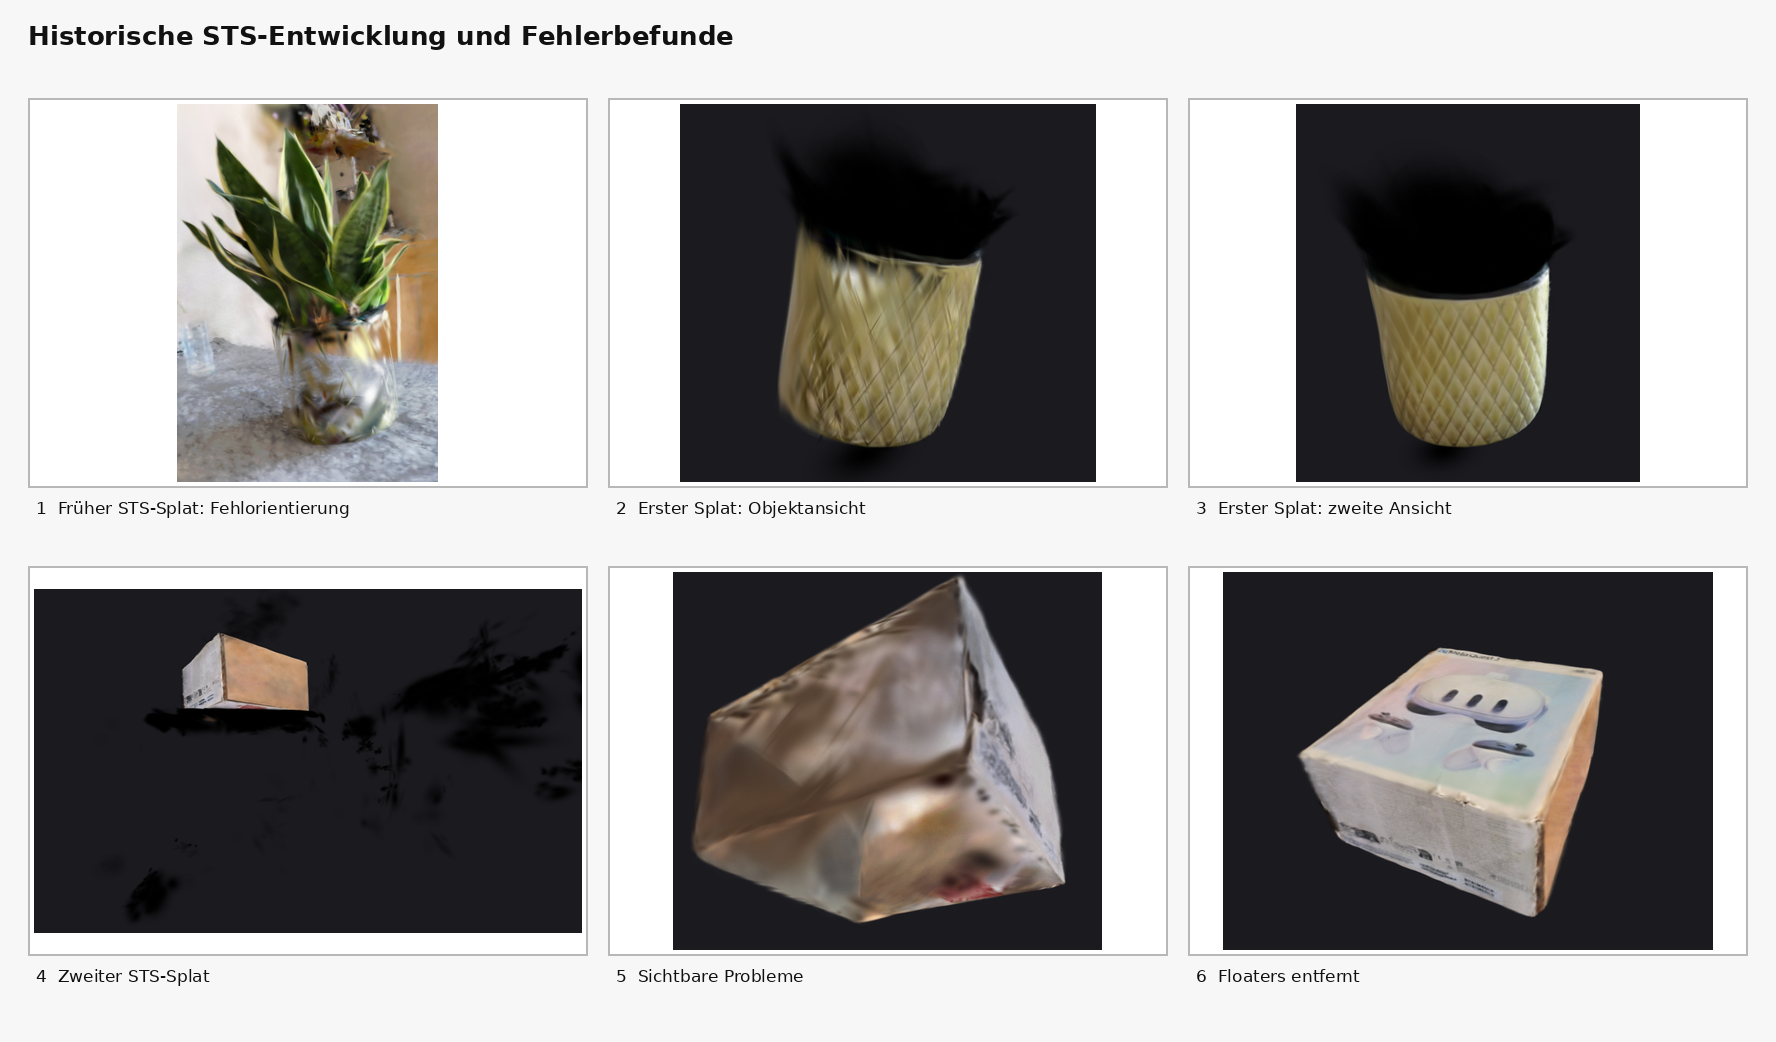
\includegraphics[width=\textwidth]{pa_panel_sts_entwicklung.png}
  \caption{Historische STS-Entwicklung: von ersten Fehlversuchen mit
  invertierter Auswahl des segmentierten Trainings (Fehlorientierung im
  Rendering) über Floaters und fehlerhafte Zwischenstände bis zu
  verlässlichen Objekt-Splats. Die Bildausschnitte stammen aus verschiedenen
  Entwicklungsständen (Juni bis Juli 2026) und untermauern die schrittweise
  Fixierung der STS-/Rendering-Datenverträge.}
  \label{fig:pa-panel-sts}
\end{figure}

\begin{figure}[H]
  \centering
  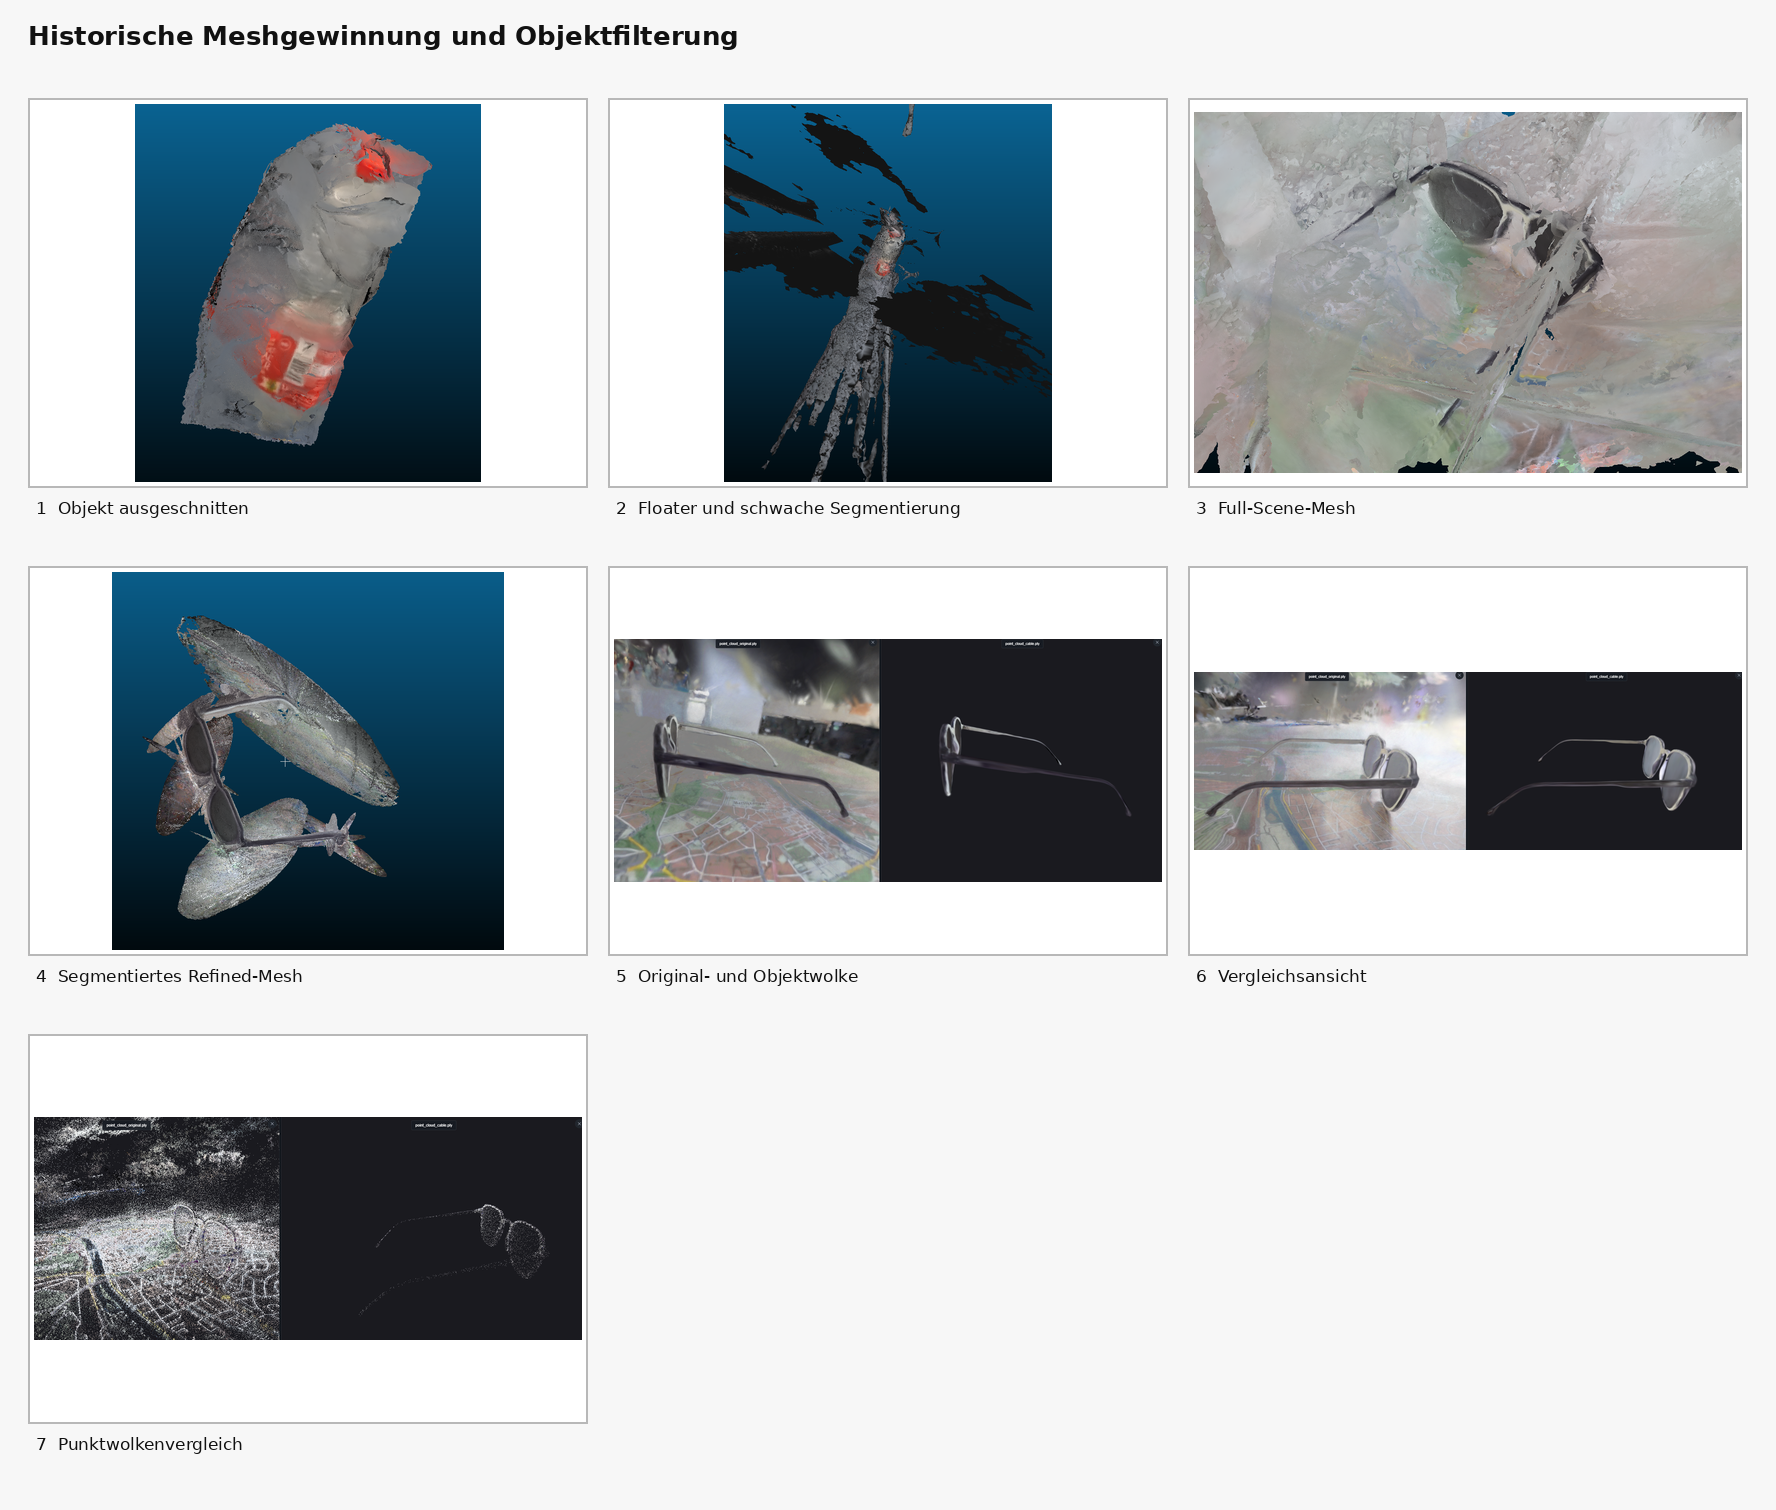
\includegraphics[width=\textwidth]{pa_panel_mesh_filterung.png}
  \caption{Historische Meshgewinnung und Objektfilterung: vom ersten
  herausgeschnittenen Objekt über schlecht segmentierte Zwischenstände und
  Floaters bis zum segmentierten Refined-Mesh der aktuellen Route.}
  \label{fig:pa-panel-mesh}
\end{figure}

Das STS-Panel (Abbildung~\ref{fig:pa-panel-sts}) zeigt den historischen
Entwicklungsweg des Renderings: Die Teilbilder 2 bis 4 dokumentieren Floater
und die Probleme ohne die später eingeführte Farbfilterung; Teilbild 5 belegt,
dass auch bei passender Segmentierung eine schlechte Aufnahme noch immer
problematische Splats erzeugen kann. Das Mesh-Panel
(Abbildung~\ref{fig:pa-panel-mesh}) dokumentiert entsprechend die Meshroute:
Teilbild 1 und 2 zeigen, wie sich SuGaR vor dem Fork verhielt und warum der
maskenbasierte Verlust nötig wurde. Teilbild 3 entstand aus einem fälschlich
übergebenen Splat, der direkt in ein Mesh umgewandelt wurde und extrem viele
Floater hinterließ. Teilbild 4 stammt von der zuerst erprobten
SuGaR-Coarse-Variante mit Zielzähler 15.000 und bewusst deaktivierter
DN-Consistency -- die lang gezogenen Strukturen entstanden dort jedoch durch
die falsche Übergabe und die fehlende Maskenbasiertheit beziehungsweise die
RGB-lastige Supervision, nicht durch die Route selbst. Die Teilbilder 5 und 6
zeigen einen Vergleich perfekt segmentierter Splats, Teilbild 7 die
zugehörige Punktwolke. Insgesamt belegen beide Panels, dass ein
funktionierendes STS-Rendering nicht selbstverständlich ist und welche
Fehlerbilder die heutigen Quality-Gates ausschließen.
\subsection{Splat-Rendering und Generierung der Bildmetriken}

Die Bildmetriken entstehen nicht im Nachgang aus dem extrahierten Dreiecksnetz,
sondern werden über automatisierte Rendering-Skripte direkt aus den
3D-Gaussian-Checkpoints auf dem festen Test-Split (\path{eval_frames.txt})
erzeugt. Die Pipeline unterscheidet dabei drei getrennte Metrik-Dateien:

\begin{enumerate}
  \item \textbf{\path{metrics/sts_masked.json} (Original-STS / Route A):}\\
        Nach Abschluss des STS-Curriculums (7000 Iterationen) wird der Standard-3DGS-
        Checkpoint \path{point_cloud/iteration_7000/point_cloud.ply} geladen. Das
        Skript \path{render_standard_splat} rendert die Ansichten des festen
        Eval-Splits -- also Kameras, deren Bilder nicht im Training enthalten
        waren; anschließend berechnet \path{evaluate_masked_splat_metrics.py} die
        objektmaskierten Werte für PSNR, SSIM und LPIPS gegen diese
        Ground-Truth-Bilder.
        Da Route~A das Mesh direkt aus diesem STS-Splat ohne weiteres Training
        extrahiert, bildet diese Datei die photometrische Qualitätsmetrik für Route~A.
  \item \textbf{\path{metrics/sugar_coarse_masked.json} (SuGaR-Coarse-Vergleich):}\\
        In der SuGaR-Vergleichsroute optimiert das Coarse-Training ($c=9000$) die
        Gaussians mit maskiertem RGB-Loss und Normalenkonsistenz und speichert das
        Ergebnis als PyTorch-Checkpoint unter
        \path{data/sugar_output/<run_tag>/coarse/9000.pt}. Das Skript
        \path{src/python/render_sugar_checkpoint.py} lädt dieses \texttt{state\_dict}
        in das \texttt{SuGaR}-Modell in Container~D und rendert denselben
        Test-Kamerasplit. Die anschließende maskierte Auswertung schreibt
        \path{sugar_coarse_masked.json}. Sie misst die Ansichtsqualität der durch
        SuGaR veränderten Gaussian-Geometrie.
  \item \textbf{\path{metrics/sugar_refined_masked.json} (SuGaR-Refined):}\\
        Diese Datei ist für das Rendering eines verfeinerten, mesh-gebundenen Splats
        (\path{refined.ply}) vorgesehen. Wurde im jeweiligen Lauf kein
        \path{refined.ply} exportiert, schreibt der Matrixrunner ein explizites
        \texttt{\{"status":"skipped","reason":"no refined.ply exported"\}}.
\end{enumerate}

Für das korrekte SuGaR-Rendering waren zwei technische Korrekturen in
\path{render_sugar_checkpoint.py} notwendig: Erstens muss der SuGaR-Quellordner
\path{/opt/sugar} vor dem Import von \texttt{sugar\_scene} explizit in den
Python-Suchpfad (\texttt{sys.path}) eingefügt werden. Zweitens liefert der
SuGaR-Rasterizer ein HWC-Tensorlayout, während \texttt{torchvision.utils.save\_image}
ein CHW-Layout erwartet; die Hilfsfunktion \texttt{as\_chw()} normalisiert die
Kanaldimension, um Tensorformfehler zu verhindern.

\subsection{Meshrouten und kompatibler Export}

Die Produktionsroute A führt keine SuGaR-Coarse-Optimierung durch. Sie nutzt
Surface-Sampling, Poisson-Rekonstruktion, Dichtebereinigung, Decimation und
Vertexprojektion. Die Legacy-Route \texttt{sugar\_coarse} wird für eine
kontrollierte Gegenüberstellung separat ausgeführt.

Route A speichert das Coarse-PLY und konvertiert es für die bestehende
Centerline-Schnittstelle zusätzlich in \texttt{refined.obj}. Dieser
Kompatibilitätsname bedeutet ausdrücklich nicht, dass ein SuGaR-Refinement
ausgeführt wurde. Die Vergleichsroute schreibt Coarse-, Refined- und
gegebenenfalls Texturartefakte getrennt.

\subsection{Centerline und Export}

Container E führt den \texttt{single}-Centerline-Modus mit einer Voxelgröße von
0,1 und einer Mindestpfadlänge von 0,75 aus. Die Eckensegmentierung ist
deaktiviert; die lokale Kurve wird als geklemmter uniformer B-Spline Grad 10
ausgegeben. Fehlt eine Transformationsmatrix, werden globale Ausgaben deutlich
als Translation-Fallback bezeichnet. Die detaillierten GeoJSON- und
Postprocessdateien befinden sich im digitalen Anlagenteil.

\subsection{Ausgewählte Robustheitsmaßnahmen}

Die Entwicklung enthielt mehrere negative Ergebnisse. Für den Haupttext sind
nicht die jeweiligen Stacktraces, sondern die daraus abgeleiteten
Schnittstellenregeln relevant. Tabelle~\ref{tab:robustheit-kern} fasst die
wichtigsten Beispiele zusammen; die ausführlichere Chronologie befindet sich
in Tabelle~\ref{tab:fehlerchronik} im Anhang.

\begin{table}[H]
\centering
\small
\begin{tabularx}{\textwidth}{p{2.5cm}XXX}
\toprule
Problem & Ursache & Korrektur & Bedeutung\\
\midrule
Leerer SuGaR-Eval-Split & Dateiendung und Kamerastem unterschieden sich &
Normalisierung und Kardinalitätsprüfung & Ein vorhandener Split ist erst nach
erfolgreichem Matching gültig.\\
Unvollständige Matrix & Unterprozesse konsumierten TSV-stdin &
stdin-unabhängige Schleifen & Geplante und tatsächlich ausgeführte Läufe müssen
getrennt geprüft werden.\\
Leere Eval-Maske & Globaler Coverage-Guard war weniger streng als der feste
Split & Split erst nach dem Warp aus nichtleeren Masken & Eval-Eignung ist ein
eigener Datenvertrag.\\
SuGaR-Renderfehler & Importpfad und HWC/CHW-Layout & expliziter Pfad und
Layoutkonvertierung & STS-Zwischenmetriken dürfen nicht als SuGaR-Ergebnis
gedeutet werden.\\
Verästeltes Skelett & Medialflächen und kurze Stachel-Äste & Durchmesserpfad im
\texttt{single}-Modus & Netzwerkobjekte bleiben außerhalb des Scopes.\\
\bottomrule
\end{tabularx}
\caption{Kernprobleme und daraus abgeleitete Robustheitsmaßnahmen.}
\label{tab:robustheit-kern}
\end{table}

\section{Versuchsaufbau}
\label{sec:versuchsaufbau}

Die Evaluation folgt einer gestuften Logik. Ein ressourcenschonender
Smoke-Test prüft zunächst die Datenverträge. Separate COLMAP-Voruntersuchungen
begründen den SfM-Standard. Danach untersuchen automatisierte Matrixläufe
Kameramodell, FPS und Auflösung. Eine kontrollierte Vierfeld-Ablation lokalisiert
den Einfluss von Gaussian-Optimierung und Tiefenroute\footnote{Die
Tiefenroute bezeichnet die Art, wie die für das Surface-Sampling benötigte
Oberflächentiefe gewonnen wird: entweder durch Projektion der
SuGaR-``Diamond''-Primitive in einen Z-Buffer (Diamond-Mesh-Tiefe) oder
direkt aus dem Gaussian-Rasterizer.}. Abschließend
vervollständigt eine zwölf Läufe umfassende SuGaR-Folgeprüfung den technischen
Meshroutenvergleich auf der Coarse-Stufe.

\subsection{Testdatensatz, Variablen und Konstanten}

Die Tests verwenden das Alurohr-Video als linearen Labor-Testdatensatz. Die
Matrixprofile bestehen aus 5 FPS und 2 FPS sowie den Auflösungen 1280$\times$720,
960$\times$540 und 640$\times$360. Der Prompt lautet \texttt{pipe}. SIFT-
Merkmale, Sequential-Overlap, Guided Matching, STS-Iterationszahl, Meshziel,
Surface-Sample-Zahl und Seed werden konstant gehalten.

\begin{table}[H]
\centering
\small
\begin{tabularx}{\textwidth}{p{3.5cm}X}
\toprule
Kategorie & Festlegung\\
\midrule
Datensatz/Prompt & Alurohr-Video, \texttt{pipe}\\
Kameramodelle & \texttt{SIMPLE\_RADIAL}, \texttt{PINHOLE}, \texttt{OPENCV}\\
Frameprofile & 2/5 FPS; $1280\times720$, $960\times540$, $640\times360$\\
COLMAP-Standard & 4096 Plain-SIFT, Overlap 15, Guided Matching aus,
Peak-Threshold 0,003\\
STS & 7000 Gesamtiterationen, 5000 Objektcurriculum\\
Mesh & 200.000 Zielvertices, 5.000.000 Surface-Samples, Poisson-Tiefe 10,
Seed 42\\
Masken & RGB \texttt{default}, DN \texttt{middle}, keine zusätzliche
Dilatation\\
Centerline & \texttt{single}, Voxel 0,1, B-Spline Grad 10\\
Bildmetriken & ausschließlich objektmaskierte PSNR, SSIM und LPIPS\\
\bottomrule
\end{tabularx}
\caption{Zentrale Variablen und kontrollierte Standardparameter.}
\label{tab:versuchsparameter}
\end{table}

Die Bildmetriken sind die einzigen Qualitätsmetriken für Renderings.
Maskenabdeckung, Registrierungsquote, Laufstatus und Laufzeit werden als
technische Zusatzgrößen geführt. Sie werden nicht zu weiteren Bildmetriken
umdefiniert.

Für die Maskenlogik werden zwei Funktionen getrennt: Die erodierte
\texttt{middle}-Maske bildet einen konservativen Objektkern und wird für das
Coverage-Gate sowie für die Auswahl nichtleerer Eval-Ansichten verwendet. Die
eigentliche Bildmetrik wird anschließend mit der weniger beschnittenen
\texttt{default}-Maske berechnet. Dadurch werden unsichere Randbereiche bei
der Zulassung eines Frames streng geprüft, ohne die Bildmetriken unnötig auf
eine erodierte Objektfläche zu beschränken. Das Feld
\texttt{mask\_level=default} in den Metrik-JSONs dokumentiert diese tatsächliche
Auswertungsmaske.

Die Maskenhierarchie selbst ist im Projektverlauf vereinheitlicht worden:
Historisch war zwischenzeitlich auch die \texttt{default}-Maske dilatiert;
verbindlich gilt nun \texttt{default} = unverändert, \texttt{middle} = einfach
erodiert, \texttt{small} = zweifach erodiert, ohne Dilatation. SuGaR nutzt
dabei nicht alle Maskenstufen gleichzeitig: Der maskierte RGB-Verlust der
Coarse-Route arbeitet auf \texttt{default}, die Depth-Normal-Consistency auf
der konservativeren \texttt{middle}-Maske.

\subsection{COLMAP-Voruntersuchung}

Eine getrennte CPU-Voruntersuchung vergleicht die Sparse-SfM-Stufe. Sie umfasst
unter anderem 4096 gegen 8192 SIFT-Merkmale, Guided Matching und zwei
Kompressionsprofile. Alle fünf ausgewerteten Hauptläufe registrierten 240 von
240 Bildern. Die Untersuchung begründet den Standard 4096 Plain-SIFT und
deaktiviertes Guided Matching, ist aber kein vollständiger STS-/Meshvergleich.

\subsection{Smoke-Test und Replay}

Der Lauf \path{matrix_smoke_low_pipe_full} ist ein einzelner Low-
Auflösungstest mit 5 FPS, \texttt{SIMPLE\_RADIAL} und Route A. Er prüft die Kette von den
idealen Masken über einen vorhandenen STS-Checkpoint bis zu Mesh, Rendering,
Metriken und Postprocessing. Der Zusatz \texttt{full} bedeutet, dass dieser
einzelne Lauf nicht nach der Maskenprüfung beendet wurde; er bezeichnet keine
vollständige Parameter-Matrix.

Der Replay startet an einer Schrittgrenze und stellt nur die dafür notwendigen
Artefakte wieder her. Dadurch können teure, bereits validierte Stufen
wiederverwendet werden, ohne einen abgebrochenen Optimierer innerhalb einer
Iteration fortzusetzen.

\subsection{Kameramodell-/FPS-/Auflösungsmatrix}

Die bereits ausgeführte A-Route wurde nicht erneut gerechnet. Die Folge-Matrix
\path{matrix_rest} enthält PINHOLE-A und OPENCV-A. Die gezielte
SuGaR-Folgeprüfung verwendet die separate Konfiguration
\path{tools/experiment_matrix_sugar.tsv} mit SIMPLE\_RADIAL-SuGaR und
OPENCV-SuGaR. Damit werden Kameramodell, FPS und Auflösung getrennt von der
Meshroute untersucht.

Die zusammengeführte Hauptauswertung enthält sechs historische
\texttt{simple\_radial\_a}-Versuche und 18 Folgeexperimente. Die Folgeexperimente
umfassen \texttt{PINHOLE}-A, \texttt{OPENCV}-A und die damalige
\texttt{SIMPLE\_RADIAL}-SuGaR-Route über jeweils drei Auflösungen und zwei
FPS-Profile. Der Runner arbeitet seriell, weil alle Versuche denselben
Live-Workspace verwenden und zwischen den Läufen archiviert und bereinigt wird.

\subsection{Vierfeld-Ablation der Meshgewinnung}

Die Ursache sichtbarer Meshunterschiede wird mit vier Coarse-only-Varianten
getrennt:

\begin{enumerate}
  \item A: Original-STS-GS mit projizierter Diamond-Mesh-Tiefe;
  \item B: Original-STS-GS mit Gaussian-Rasterizer-Tiefe;
  \item C: SuGaR-Coarse $c=9000$ mit Diamond-Mesh-Tiefe;
  \item D: SuGaR-Coarse $c=9000$ mit Gaussian-Rasterizer-Tiefe.
\end{enumerate}

Kameras, Eingabemasken, Surface-Level, Poisson-Tiefe, Dichtequantil,
Vertexziel, Samplezahl, Projektion und Seed bleiben konstant. Dadurch werden
Gaussian-Optimierung und Tiefenroute als getrennte Einflussfaktoren untersucht.
Die aus gleichmäßig gesampelten Meshpunkten berechneten gerichteten Distanzen
sind relative Vergleichsgrößen zwischen den Varianten, keine Abweichungen von
einer Ground Truth.

\subsection{Abgeschlossene SuGaR-Folgeprüfung}

Die Folgematrix umfasst zwölf Läufe über die Kameramodelle
\texttt{SIMPLE\_RADIAL} und \texttt{OPENCV} (jeweils mit
\texttt{sugar\_coarse}) bei drei Auflösungen und zwei FPS-Profilen. Alle zwölf
Manifeste und Coarse-Metrikdateien sind erfolgreich
archiviert. Ein verfeinertes PLY wurde in diesen Läufen nicht exportiert; die
Folgematrix bewertet daher nur die Coarse-Route. Die Ergebnisse zeigen die
Grafiken in Abschnitt~\ref{sec:sugar-folgepruefung} und die Fehlerchronik in
Tabelle~\ref{tab:fehlerchronik}.

\subsection{Evaluationsprotokoll}

Für jeden Lauf werden Masken- und Warp-Coverage sowie die COLMAP-Ausgaben
archiviert. Hinzu kommen STS-Checkpoint (\path{point_cloud.ply}), gegebenenfalls
SuGaR-Coarse-Checkpoint (\path{9000.pt}), Mesh-/Postprocess-Ausgaben, feste
Eval-Frames und objektmaskierte PSNR-, SSIM- und LPIPS-Werte. Die Daten werden über
\texttt{manifest.json}, \texttt{parameters.json}, \texttt{run.log} und
\texttt{run.md} nachvollziehbar gehalten.

Die Matrixgrafiken verwenden den arithmetischen Mittelwert aus 2 und 5 FPS nur,
wenn beide Läufe derselben Konfiguration vollständig erfolgreich waren. Ein
technischer Fehler wird nicht als schlechter Qualitätswert in einen Mittelwert
umgewandelt. Die neue Auswertung trennt zusätzlich die Modellstufen: Eine
STS-Grafik liest ausschließlich die aus \path{point_cloud.ply} gerenderten
\texttt{sts\_masked.json}-Dateien (Route~A), eine SuGaR-Grafik ausschließlich die
aus \path{9000.pt} gerenderten \texttt{sugar\_coarse\_masked.json}-Dateien. Da
beide Formate dieselben 3D-Gaussian-Parameter speichern, beruht der Unterschied
in den Messwerten (rund $29{,}5\,\mathrm{dB}$ gegenüber $21{,}5\,\mathrm{dB}$)
rein auf den veränderten Gaussian-Parametern nach der SuGaR-Coarse-Optimierung und
nicht auf dem Dateiformat. Die \texttt{per\_frame}-Werte werden ergänzend als
Boxplots mit Einzelpunkten dargestellt, damit Streuung und Ausreißer nicht durch
den Mittelwert verborgen werden.

Ein Lauf erhält nur dann den Status vollständig erfolgreich, wenn alle für
seine Route vorgesehenen Stufen gültig sind: Masken und Coverage,
COLMAP-Modell, Roh-/Ideal-Domäne, vollständig gematchter Eval-Split,
STS-Checkpoint, Objektselektion, Mesh, Postprocessing, objektmaskierte Metriken
und Ergebnisarchiv. Für SuGaR-Coarse muss zusätzlich das SuGaR-Rendering
erfolgreich sein. Eine zuvor erzeugte \texttt{sts\_masked.json} bleibt eine
STS-Baseline und wird nicht als SuGaR-Messung gewertet.

\subsection{Erfolgskriterien der Projektarbeit}

Die PA gilt als technisch erfolgreich, wenn:

\begin{enumerate}
  \item die zentrale Pipeline für den Testdatensatz durchläuft;
  \item die Bild- und Maskendomänen konsistent sind;
  \item STS, Meshgewinnung und Centerline-Extraktion reproduzierbar arbeiten;
  \item der Status jedes Matrixlaufs und die Fehlerursache archiviert sind;
  \item die Ergebnisse für eine spätere GNSS-basierte Bachelorbewertung
        geeignet abgelegt werden.
    \item interaktiver Vollauf, Replay, Autopilot und Matrixrunner in ihrer
      jeweiligen Funktion eindeutig dokumentiert und mindestens über einen
      archivierten Lauf oder Vertragstest nachgewiesen sind.
\end{enumerate}

Die PSNR-/SSIM-/LPIPS-Werte sind dabei Funktions- und Visualisierungsmetriken.
Sie ersetzen nicht die spätere geometrische Bewertung mit Centerline-RMSE,
Hausdorff-Distanz und GNSS-Referenz.

\section{Ergebnisse}

\subsection{Repräsentative End-to-End-Artefaktkette}

Der vollständige Funktionsnachweis wird anhand eines intern konsistenten
Referenzlaufs dargestellt. Die endgültige Fassung zeigt dafür dieselbe
Verarbeitungskette in aufeinander abgestimmten Ansichten: Rohframe,
\texttt{default}/\texttt{middle}-Maske, ideale Bild-/Maskendomäne,
COLMAP-Sparse-Modell, objektbezogene STS-Gaussians, Route-A-Coarse-Mesh sowie
lokale Centerline und Grad-10-B-Spline. Eine solche Kette ist für alle drei
Auflösungsstufen visuell dokumentiert; Anhang~\ref{app:durchlauf} zeigt den
vollständigen Pipeline-Durchlauf mit 5 FPS und OPENCV in 720p, qHD und Low.

Die archivierten Läufe verwenden durchgängig 240 Kameras; davon dienen 210 dem
Training und 30 der Evaluation. Der feste Eval-Split und seine Begründung sind
in Kapitel~\ref{sec:versuchsaufbau} beschrieben; hier genügt die Erinnerung,
dass die Evaluationsbilder gerade deshalb bewertbar sind, weil sie nicht am
Training beteiligt waren. Jede archivierte Kette erzeugte Route-A-Mesh,
Rendering, objektmaskierte Metriken, Centerline, B-Spline und GeoJSON. Der
Autopilotnachweis selbst ist über sechs archivierte Autopilot-Volläufe erbracht
(Abschnitt~\ref{sec:versuchsaufbau}); die Visualisierung dieser Durchläufe in
ausgewählten Screenshots liegt ebenfalls im Anhang~\ref{app:durchlauf}. Die
historischen Zwischenstände, die zu den heutigen Einstellungen in STS,
Objektfilterung und SuGaR geführt haben, sind in
Kapitel~\ref{sec:implementierung} sowie in
Abschnitt~\ref{sec:sugar-folgepruefung} dokumentiert.

\subsection{Visueller Vergleich der Auflösungsvarianten}
\label{sec:visueller-aufloesungsvergleich}

Die visuelle Gegenüberstellung der drei Auflösungen ist in
Anhang~\ref{app:durchlauf} entlang derselben Verarbeitungskette dokumentiert.
Bei
den Masken ist in den höher aufgelösten Varianten eine feinere Kontur- und
Randlokalisierung erkennbar. In keiner der drei Varianten treten jedoch
offensichtliche gravierende Fehler wie eine vollständig leere Maske, ein
Verlust des Zielobjekts oder große Ausrisse auf. In der \texttt{low}-Variante
wird zusätzlich das Verbindungskabel zwischen den Rohren in die Objektmaske
aufgenommen. Streng semantisch ist dies eine Übersegmentierung; da das Kabel
direkt zum dargestellten Objektverbund gehört, wird dieser Anteil für die
qualitative Pipelinebewertung als vertretbar behandelt.

In den Übersichten der COLMAP-Punktwolken sind zwischen den Auflösungen keine
direkten, großräumigen Unterschiede zu erkennen. Dies ist mit dem festgelegten
SIFT-Limit von 4096 Merkmalen pro Bild vereinbar: Eine höhere Pixelauflösung
führt nicht automatisch zu einer proportional größeren Punktwolke. In der
vergrößerten Darstellung fällt jedoch auf, dass in der linken unteren
Wandecke der \texttt{720p}-Variante mehr Punkte sichtbar sind. Dies kann darauf
hindeuten, dass das begrenzte Merkmalsbudget dort anders und räumlich breiter
über die ansonsten gleichförmige Fläche verteilt wird. Eine breitere Verteilung
homologer Bildpunkte könnte die Track-Stabilität und damit die interne
Geometriekonsistenz des SfM-Modells begünstigen. Aus den Screenshots allein
folgt daraus jedoch kein Nachweis einer höheren absoluten geometrischen
Korrektheit; dafür wären insbesondere Trackstatistiken, räumliche
Korrespondenzverteilungen und eine unabhängige Referenz erforderlich.

Bei den Splats ist der auffälligste Unterschied in der \texttt{low}-Variante
die bereits genannte Aufnahme des Verbindungskabels. Außerdem unterscheiden
sich die oberen Objektkanten: In den höher aufgelösten Varianten wirkt die
Objektgeometrie über die Blickwinkel hinweg konsistenter aufgenommen, während
die \texttt{low}-Variante am unteren rechten Bildrand einen zusätzlichen
Floater zeigt. Die höher aufgelösten Splats wirken dadurch in dieser
Gegenüberstellung geometrisch sauberer. Auch diese Aussage ist als visueller
Befund und nicht als unabhängige Genauigkeitsmessung zu verstehen.

Die Meshbilder zeigen eine entsprechende Übertragung der Unterschiede, weil
die hier dargestellte Route~A das Mesh unmittelbar aus den STS-Splats ableitet.
In den Detailansichten weist die niedrigste Auflösung die ungenaueste und
zackigste Oberfläche mit mehreren Spitzen auf. Die \texttt{qHD}-Variante wirkt
in der betrachteten Ansicht überraschend glatt und insgesamt visuell am
geschlossensten. Die \texttt{720p}-Variante erscheint dagegen besonders klar
durch die Maskengrenze begrenzt: Aufgenommene Bereiche besitzen deutliche
Kanten, ohne dass ein starkes Glätten oder Ausfransen entsteht. Dieses
Ausfransen ist bei der \texttt{low}-Centerline am deutlichsten; sie enthält
mehr Richtungswechsel und Ecken. Die Centerlines von \texttt{720p} und
\texttt{qHD} unterscheiden sich visuell dagegen nur gering. Die Befunde sind
qualitativ und ersetzen keine Vermessung gegen eine unabhängige Centerline.

\subsection{COLMAP-Voruntersuchung}

Ebenso wurde vor den Matrixläufen eine Versuchsreihe mit COLMAP gestartet;
dabei wurde geprüft, inwiefern sich einzelne Einstellungen im Hinblick auf den
zeitlichen Aufwand und die Qualität der Sparse-Rekonstruktion lohnen. Alle
fünf dokumentierten Hauptläufe registrierten 240 von 240 Bildern; die
vollständige Tabelle steht in Anhang~\ref{tab:colmap-vorstudie}. Guided
Matching erhöhte die Sparse-Punktzahl gegenüber Plain-SIFT 4096 nur um rund
1,98\,\%, benötigte aber nahezu die doppelte Zeit und erhöhte den mittleren
Reprojektionsfehler. 8192 Merkmale lieferten etwa 0,82\,\% mehr Punkte bei
5,5\,\% mehr Laufzeit.

Diese Beobachtungen widersprechen einander nicht: Bei fixiertem
Merkmalslimit ist die Anzahl detektierter Merkmale pro Bild weitgehend
identisch, weshalb die Punktzahl kaum steigt -- mehr Eingabemerkmale führen
nicht automatisch zu mehr 3D-Punkten. Guided Matching ergänzt zusätzlich
Korrespondenzen an schwierigen Stellen; dass dabei der mittlere
Reprojektionsfehler leicht ansteigt, zeigt, dass diese zusätzlichen Matches
im Mittel schwerer zu konsistenten Spuren zu bündeln sind als das
Grundmuster. Beides zusammen rechtfertigt für den Projektstand den Standard
Plain-SIFT 4096 ohne Guided Matching: gleiche Registrierungsqualität bei
geringerer Laufzeit und einfacherer Fehlerdiagnose.

\subsection{Objektmaskierte Bildmetriken}

Ein Matrixlauf ist ein vollständig protokollierter Einzelversuch für genau
eine Kombination aus Kameramodell, FPS, Auflösung und Meshroute. Der Runner
erzeugt dafür einen isolierten Frame- und Maskensatz, führt COLMAP, die ideale
Bilddomäne, STS, die gewählte Meshroute, Rendering und objektmaskierte
Metriken aus und archiviert anschließend die Resultate. In der Entwicklung
traten unter anderem ein durch Unterprozesse konsumierter TSV-Standardinput,
leere feste Eval-Masken sowie ein SuGaR-Import-/Tensorlayoutfehler auf. Diese
Fehler wurden durch stdin-unabhängige Schleifen, einen nichtleeren festen
Eval-Split sowie die Korrektur des Renderhelfers behoben. Dadurch lassen sich
die Matrixläufe heute mit denselben Parametern erneut erzeugen und unter
identischen Kriterien vergleichen.

Die Matrix dient dabei nicht dazu, aus einer einzelnen Bildmetrik eine
„beste“ Pipeline zu küren. Sie zeigt, welche Kombinationen technisch
durchlaufen, welche Fehlerfälle auftreten und wie sich die Ansichtsmetriken
unter kontrollierten Änderungen verhalten. Die Produktionsentscheidung für
Route A stützt sich deshalb vor allem auf die A/B/C/D-Geometrieablation und
den direkten Erhalt der STS-Gaussian-Geometrie; die Matrix ergänzt diesen
Befund um Robustheit und reproduzierbare Vergleichswerte.

Die STS-Grafik verwendet ausschließlich \path{sts_masked.json}, die
SuGaR-Grafik \path{sugar_coarse_masked.json}; die Interpretation der drei
Ansichtsmetriken und ihre Grenzen wurden bereits in
Kapitel~\ref{sec:grundlagen} definiert und werden hier nicht wiederholt.
Für die Meshentscheidung sind zusätzlich Vertex-/Face-Struktur, relative
Meshabstände und die visuelle Artefaktprüfung maßgeblich.

Ein erneuter vollständiger Matrixlauf ist als Wiederholungsprüfung sinnvoll.
Bei nominal gleichen Parametern sind kleine Abweichungen durch stochastische
Optimierung, Surface-Sampling sowie Software- und Hardwarestände möglich. Eine
Abweichung wird erst dann als technisch relevant bewertet, wenn Commitstände,
Eval-Split, Framezahl, Maskenabdeckung und Seeds übereinstimmen. Für die PA
werden daher nicht alle wiederholten Arbeitskopien als eigenständige
wissenschaftliche Ergebnisse benötigt; entscheidend sind die standardisierten
Metriken, die Endprodukte und die reproduzierbaren Metadaten.

Die zentrale Metrikübersicht ist nun nach Modellstufe getrennt. Die STS-Grafiken
lesen ausschließlich vollständige Original-GS-Route-A-Läufe aus
\texttt{sts\_masked.json}; die SuGaR-Grafiken lesen ausschließlich
\texttt{sugar\_coarse\_masked.json}. Vorhandene STS-Dateien aus später
fehlgeschlagenen SuGaR-Routen bleiben als Fehlernachweis archiviert, werden aber
nicht zusätzlich in der STS-Auswertung dargestellt. Die beiden FPS-Profile und
die jeweilige Runauflösung bleiben sichtbar; ein globales Ranking über
verschiedene Auflösungen wird nicht vorgenommen.

\begin{figure}[H]
  \centering
  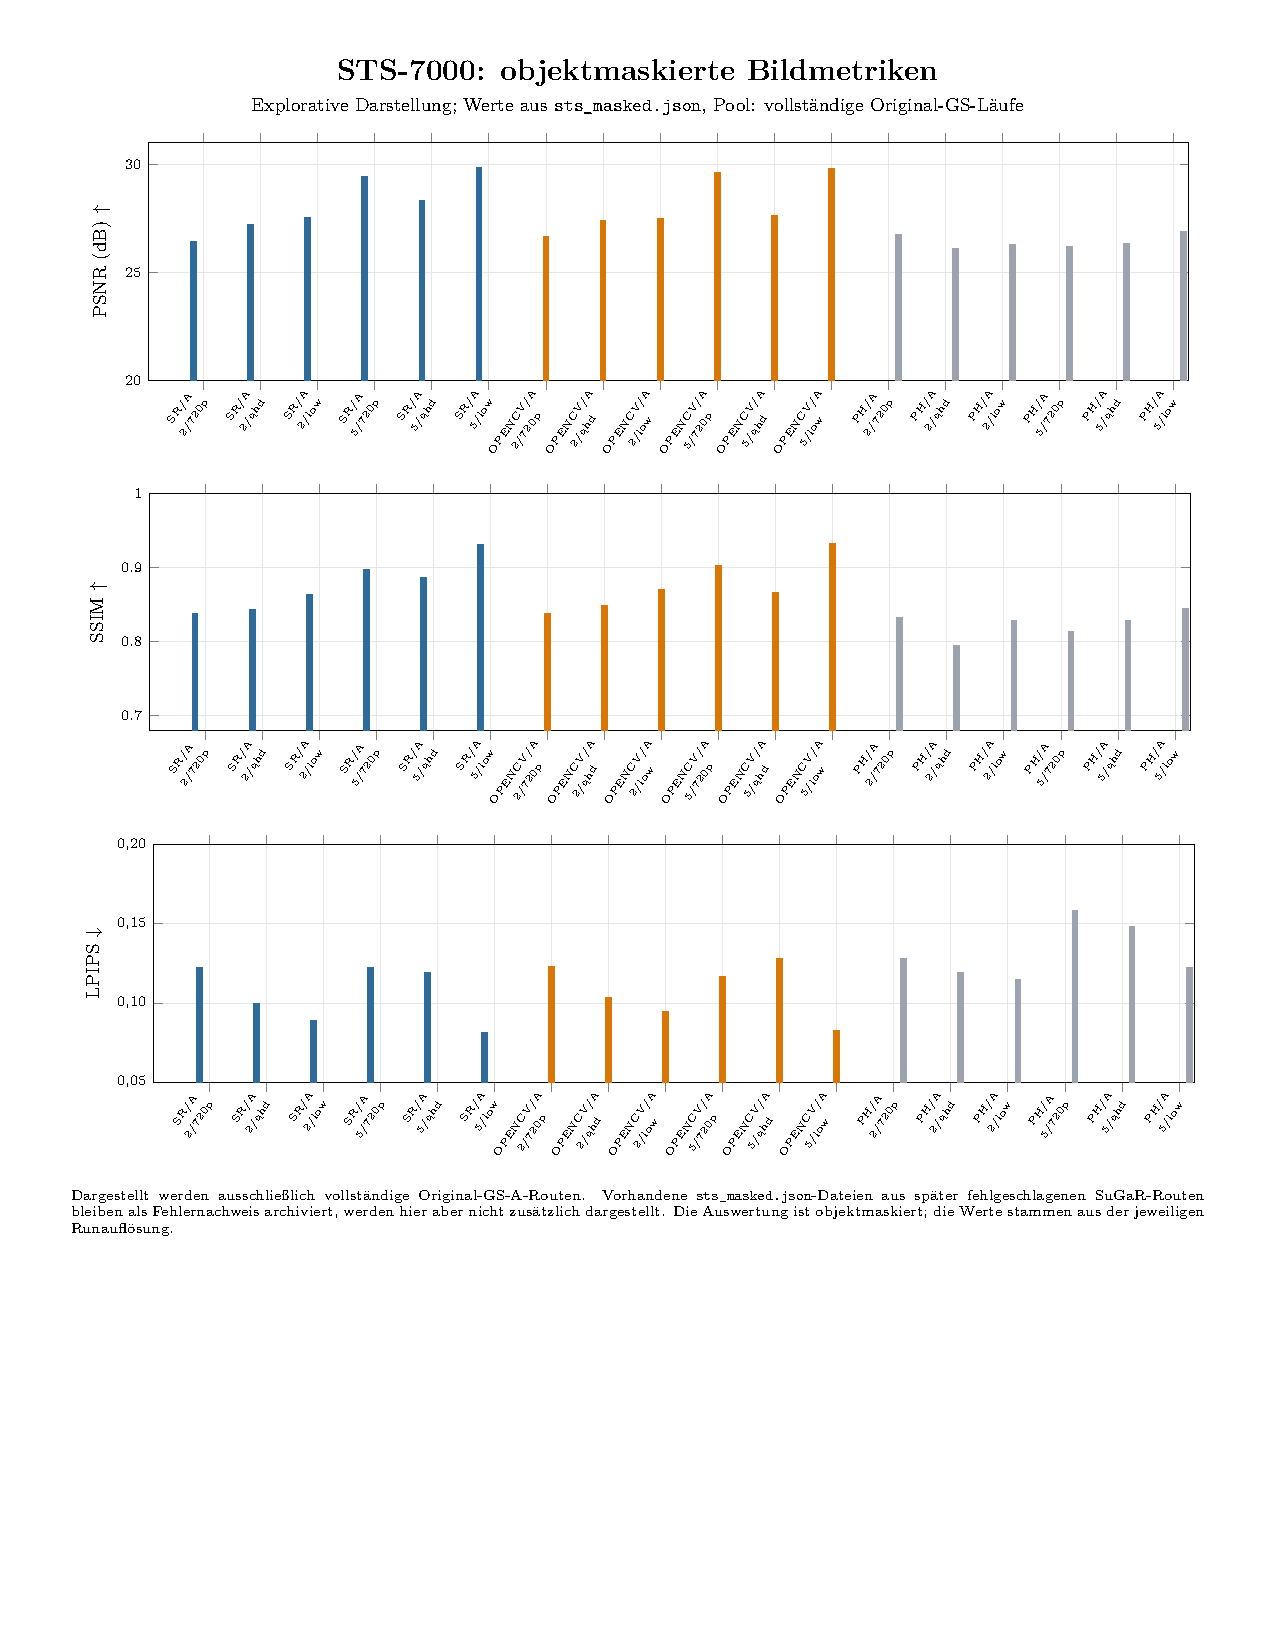
\includegraphics[width=\textwidth]{sts_masked_overview.pdf}
  \caption{Getrennte STS-7000-Auswertung der vollständigen Original-GS-Route A
  aus den archivierten \texttt{sts\_masked.json}-Dateien.}
  \label{fig:pa-matrix-overview}
\end{figure}

\begin{figure}[H]
  \centering
  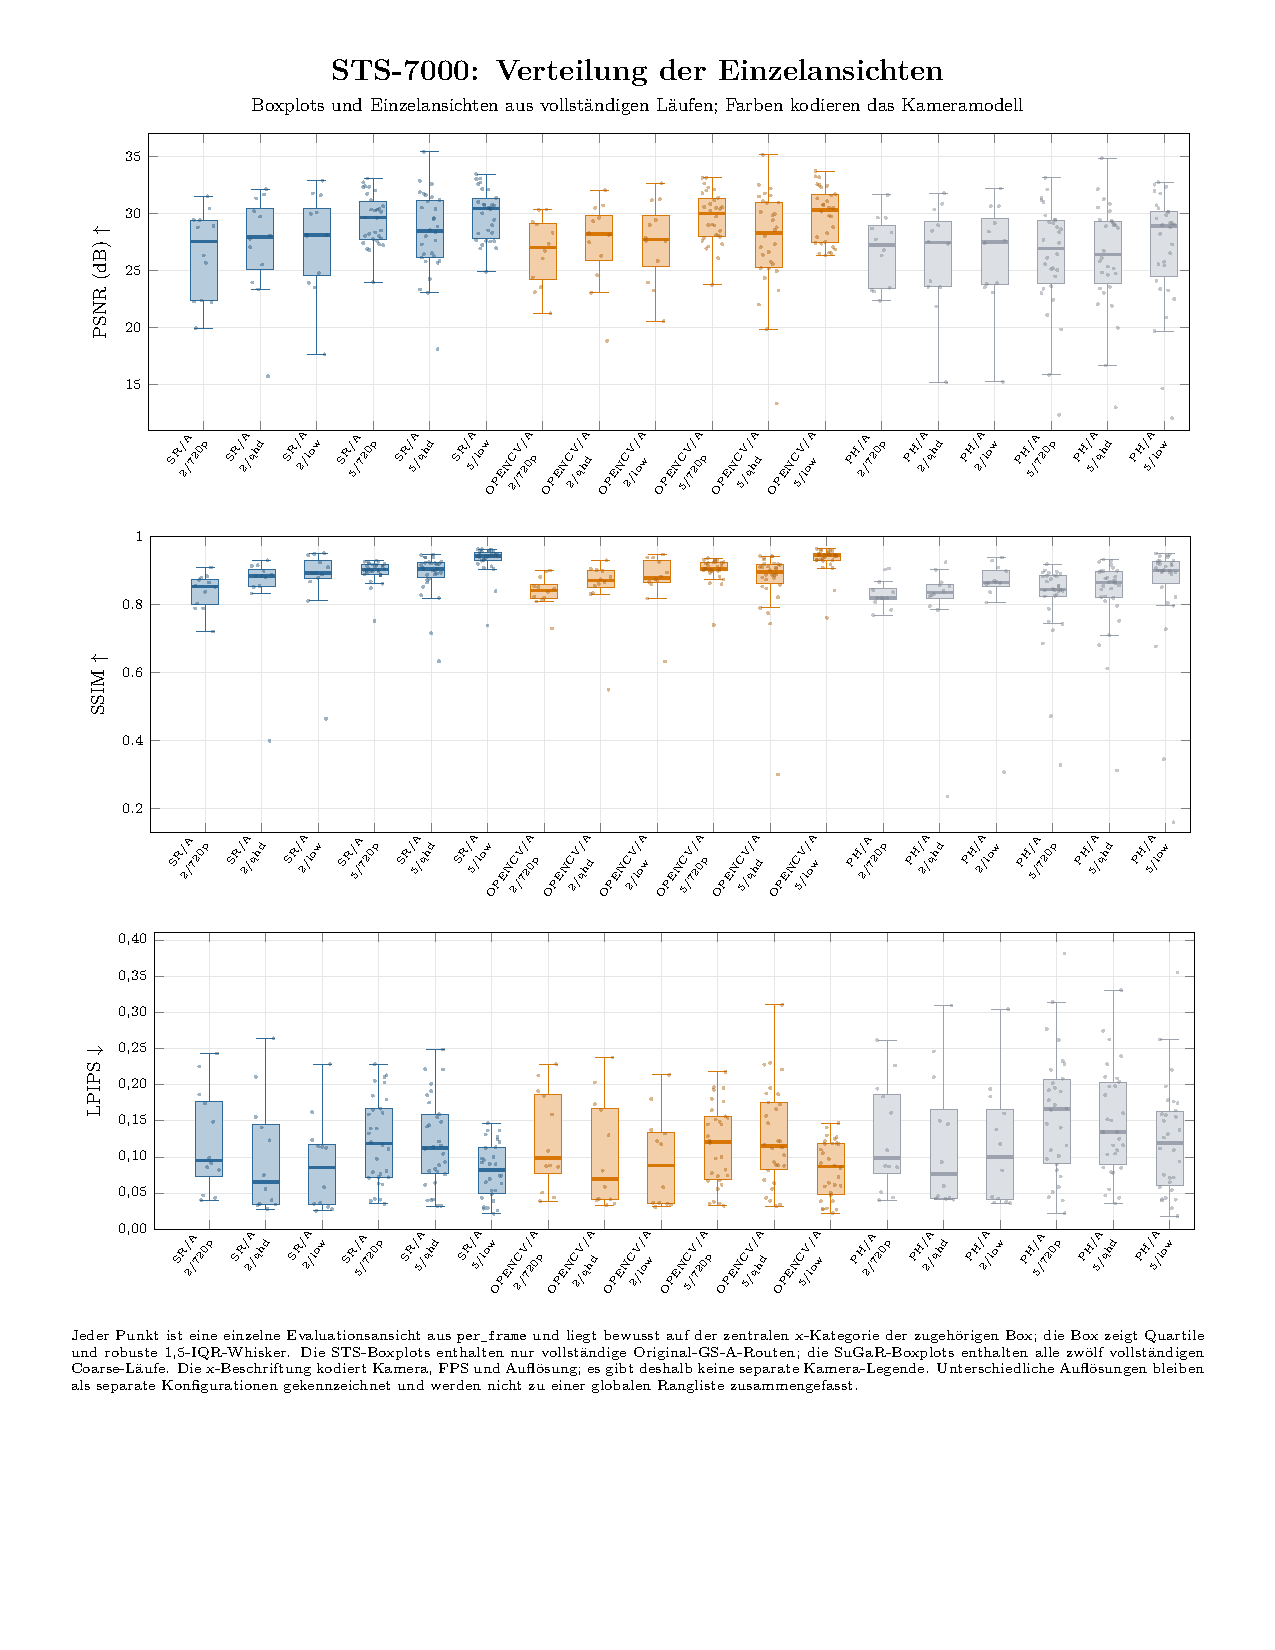
\includegraphics[width=\textwidth]{sts_masked_per_frame_boxplots.pdf}
  \caption[STS-Einzelansichten]{Verteilung der Einzelansichten in den
  vollständigen Original-GS-Route-A-Läufen. Punkte entsprechen den in
  \texttt{per\_frame} archivierten Ansichtsmetriken. SR ist blau, OPENCV
  orange und PINHOLE grau dargestellt.}
  \label{fig:pa-sts-boxplots}
\end{figure}

\begin{figure}[H]
  \centering
  
\includegraphics[width=\textwidth]{sugar_coarse_masked_overview.pdf}
  \caption{Getrennte SuGaR-Coarse-9000-Auswertung. Die STS-Baseline wird
  nicht als SuGaR-Wert verwendet.}
  \label{fig:pa-sugar-overview}
\end{figure}

\begin{figure}[H]
  \centering
  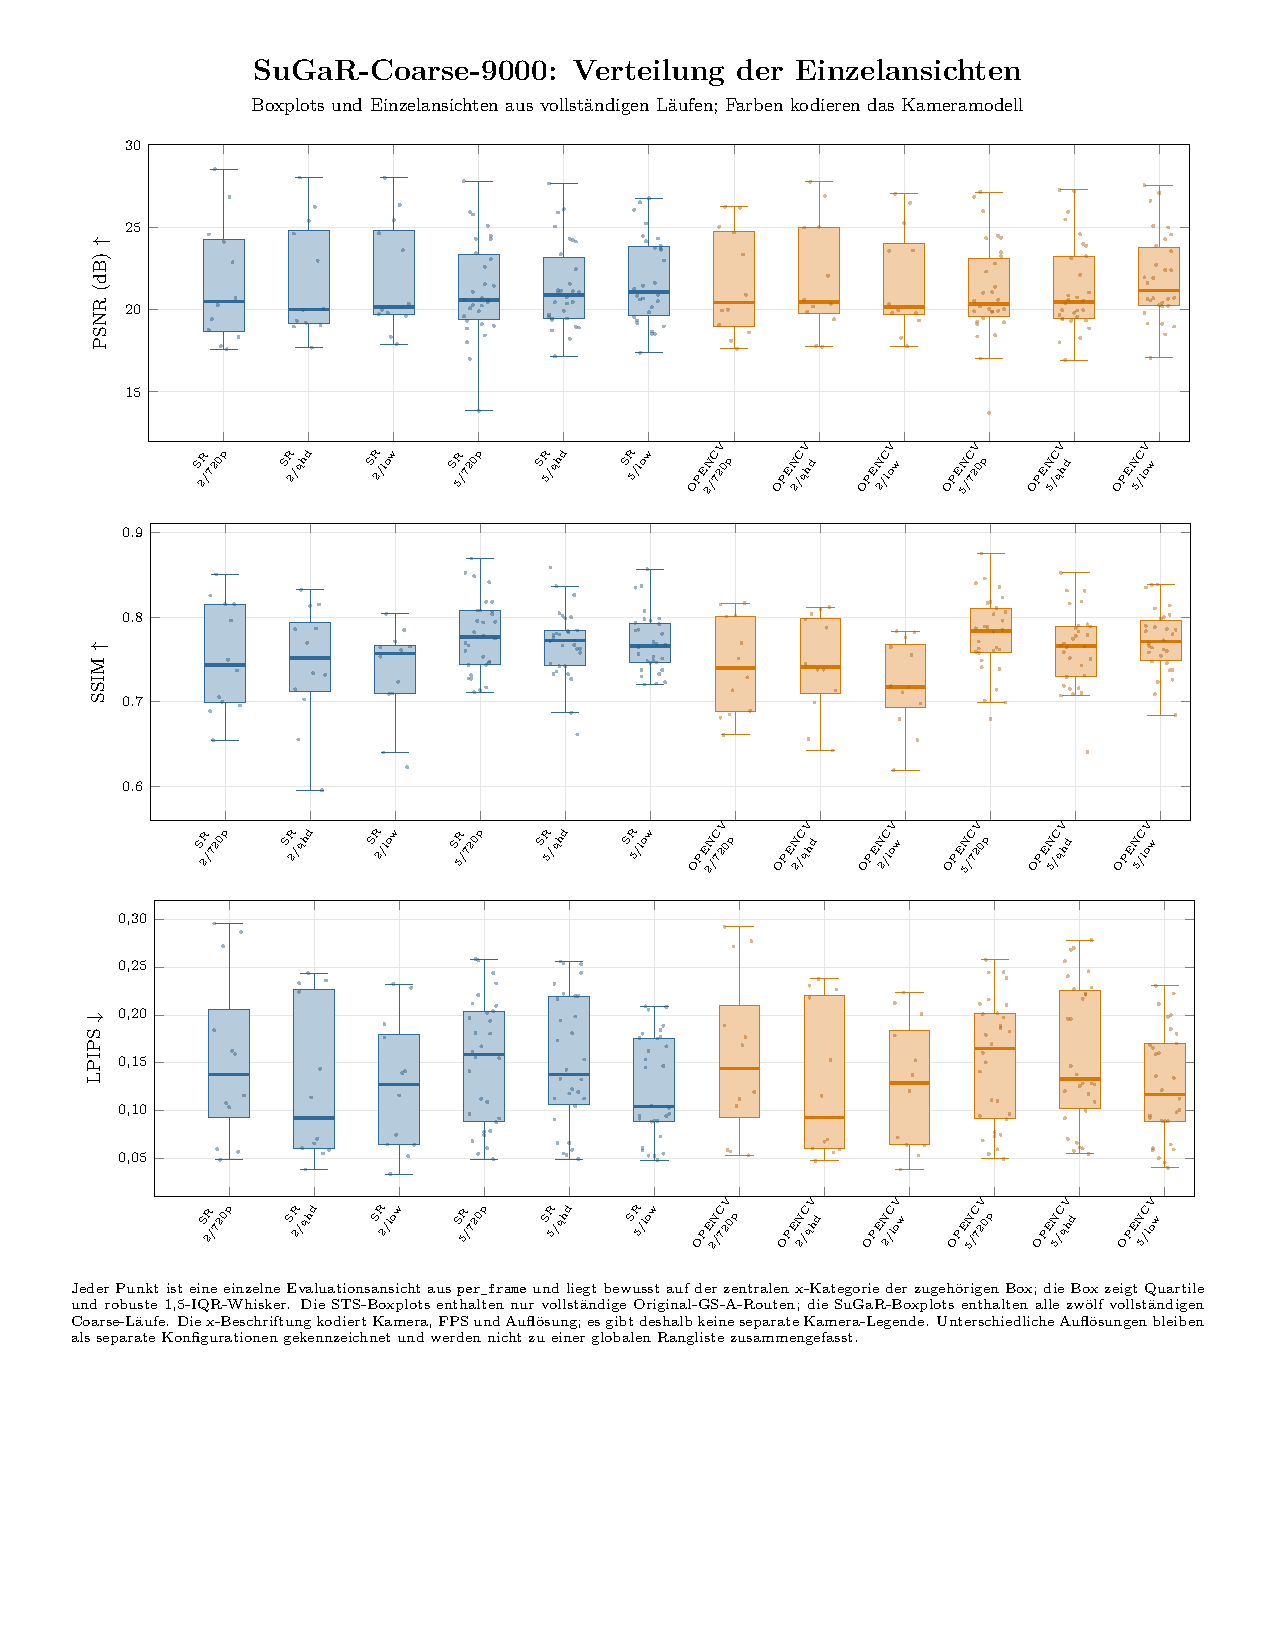
\includegraphics[width=\textwidth]{sugar_coarse_masked_per_frame_boxplots.pdf}
  \caption[SuGaR-Coarse-Einzelansichten]{Verteilung der Einzelansichten in
  den zwölf SuGaR-Coarse-Läufen. Punkte entsprechen den in
  \texttt{per\_frame} archivierten Ansichtsmetriken.}
  \label{fig:pa-sugar-boxplots}
\end{figure}

Die Boxplotpunkte liegen jeweils in der x-Kategorie ihres Laufs und werden nur
leicht horizontal verteilt; die y-Achsen berücksichtigen alle archivierten
Einzelwerte einschließlich Ausreißern.

Die deutlich niedrigeren SuGaR-Werte gegenüber den STS-Werten sind kein
direkter Widerspruch. Die beiden Dateien beschreiben unterschiedliche
Modellstufen: Der STS-Splat wird vor der zusätzlichen SuGaR-Optimierung und dem
SuGaR-Rendering ausgewertet. Im vollständigen Repeat-Lauf beträgt der
beispielhafte 5-FPS-720p-Wert für SIMPLE\_RADIAL 29,43 dB PSNR, 0,897 SSIM und
0,122 LPIPS im STS-Splat; der zugehörige SuGaR-Coarse-Wert beträgt 21,22 dB,
0,778 SSIM und 0,151 LPIPS. Die Repeat-Grafiken verwenden diese getrennten
Metrikdateien fachlich korrekt. Ältere STS-Baselines aus fehlgeschlagenen
SuGaR-Routen bleiben historisch nachvollziehbar, werden aber nicht als
SuGaR-Ergebnisse bezeichnet.

In der jeweiligen Runauflösung zeigt OPENCV-A-Low bei 5 FPS besonders hohe
Bildmetriken. Bei SIMPLE\_RADIAL und OPENCV bezieht sich die Auswertung dabei
auf die ideale, gewarpte Bilddomäne; „jeweilige Runauflösung“ bezeichnet nur
die Pixelauflösung innerhalb dieser Domäne. Dieser Befund ist ein
Screening-Ergebnis. Niedrige Auflösung kann Kantenversatz und hochfrequente
Fehler glätten, sodass bessere Bildmetriken nicht automatisch eine bessere
3D-Geometrie bedeuten. Die Werte werden daher nicht als alleinige
Produktionsentscheidung verwendet.

Die Metrikwerte verhalten sich nicht monoton über die Konfigurationen: 5 FPS
liefern nicht in jeder Kombination den numerisch besten Wert, und Low-Auflösung
ist nicht in jedem Modell besser als qHD. Die beobachteten Unterschiede
entstehen daher wahrscheinlich aus einer Interaktion von Bildauflösung,
zeitlicher Überdeckung, konkreter Kamerabewegung, Kameramodell und
STS-Optimierung. Die Maskensegmentierung selbst blieb davon unberührt stabil –
das Rohr wurde in jedem Frame erkannt. Ein isolierter Kausalnachweis für einen
einzelnen Faktor liegt nicht vor.

\subsection{Produktionskonfiguration aus der Matrixauswertung}
\label{sec:produktionskonfiguration}

Auf Grundlage der Matrixauswertung wurde die Produktionskonfiguration auf
\texttt{OPENCV}, 5 FPS und Route A festgelegt. Im Repeat-Lauf erzielen die
\texttt{OPENCV}-A-Läufe bei 720p die höchsten objektmaskierten STS-Metriken
der untersuchten Kameramodelle (29,62\,dB PSNR, 0,902 SSIM und 0,117 LPIPS;
\texttt{SIMPLE\_RADIAL}: 29,43\,dB, 0,897 und 0,122); die
Konfiguration ist über die archivierten Läufe reproduzierbar belegt. Die
Umstellung bleibt dennoch eine datengestützte Projektentscheidung ohne
unabhängige geometrische Referenz: Bei qHD liegt \texttt{SIMPLE\_RADIAL} mit
28,32\,dB vor \texttt{OPENCV} (27,63\,dB), was die nichtmonotone Interaktion
von Auflösung und Kameramodell unterstreicht. Der Standard gilt daher
ausdrücklich für die Produktionsauflösung 720p bei 5 FPS.

Eine nachträgliche Analyse des archivierten 720p-OPENCV-Sparse-Modells ergab
240 registrierte Bilder, 133.723 3D-Punkte, 890.377 Beobachtungen und einen
mittleren Reprojektionsfehler von 0,706\,Pixel. Die entsprechenden Werte lagen
bei \texttt{SIMPLE\_RADIAL} bei 0,707\,Pixel und bei \texttt{PINHOLE} bei
0,705\,Pixel. Alle drei Modelle beschreiben die beobachteten
Bildkorrespondenzen damit fast identisch und mit einem Fehler, der klein
gegenüber der Bildbreite ist; ein absoluter Schwellenwert, ab dem man von
einer „guten" Anpassung sprechen dürfte, existiert jedoch nicht. Der geringe
Unterschied entscheidet daher nicht, welches Modell das reale Objektiv
physikalisch korrekt beschreibt.
Die Reprojektionswerte sind eine Konsistenzprüfung des SfM-Modells und keine
unabhängige Kalibrierung.

Für eine belastbare Aussage über die tatsächliche Verzeichnung wären deshalb
zusätzliche Referenzdaten erforderlich, etwa eine unabhängige
Checkerboard- oder ChArUco-Kalibrierung mit denselben Aufnahmeparametern,
eine Prüfung gerader Kanten vor und nach der Entzerrung oder eine Auswertung
auf zurückgehaltenen Bildkorrespondenzen. Ohne diese Referenz bleibt
\texttt{OPENCV} eine begründete, intern konsistente Produktionsentscheidung
und kein messtechnisch validiertes Kameramodell.

Für die drei Kameramodelle des Repeat-Laufs ergeben sich gemittelte Laufzeiten
von rund 2011 Sekunden (720p), 1650 Sekunden (qHD) und 1199 Sekunden (low).
Diese Werte fließen in die Lauf-Preset-Abfrage
des CLI ein (Kapitel~\ref{sec:implementierung}), mit der zwischen
Bildauflösung und Rechenaufwand gewählt werden kann. Als reine Schrittzeiten
von STS bis Postprocessing ersetzen sie keine vollständige End-to-End-
Zeitmessung.

\subsection{Gemessene End-to-End-Laufzeiten}
\label{sec:laufzeiten-e2e}

Für vollständige End-to-End-Zeiten wurde der Verifikationsbatch
\path{matrix_e2e_verifikation_260826} ausgeführt: drei Matrixläufe der
Produktionskonfiguration (Route A, \texttt{OPENCV}, 5 FPS) über die drei
Auflösungen, jeweils inklusive SAM~3.1, COLMAP, Maskenwarp, Rendering und
Archivierung. Tabelle~\ref{tab:e2e-laufzeiten} fasst die aus dem Batch-Log
rekonstruierten Phasenzeiten zusammen; die Nachlaufphase ist als Obergrenze bis
zum Folgesegmentbeginn ausgewiesen.

\begin{table}[H]
\centering
\small
\begin{tabularx}{\textwidth}{lrrrr}
\toprule
Auflösung & Kopf (SAM3+COLMAP+Warp) & STS--Post & Nachlauf & Gesamt\\
\midrule
720p & 7:49 & 32:23 & $\le$0:52 & $\approx$40:25\\
qHD  & 7:17 & 26:24 & $\le$0:44 & $\approx$33:52\\
low  & 5:27 & 18:11 & --        & $\approx$23:46\\
\bottomrule
\end{tabularx}
\caption{Gemessene End-to-End-Laufzeiten der Produktionskonfiguration
(Verifikationsbatch \path{matrix_e2e_verifikation_260826}, Quelle
\path{e2e_times.csv}). Die Nachlaufphase umfasst Render-, Eval- und
Archivierungsschritte bis zum Folgesegmentbeginn.}
\label{tab:e2e-laufzeiten}
\end{table}

Die Werte bestätigen die Preset-Angabe des CLI und werden durch den
unabhängigen Batch \path{matrix_qualitaetsvergleich_20260818} gestützt, dessen
Segmentlogs nach derselben Methode 40:16, 34:35 und 24:02 Minuten ergeben. Die
Kopfphase skaliert erwartbar mit der Auflösung; die STS--Post-Zeiten dominieren
den Gesamtlauf mit 80--82\,\%. Die timeshare-Angaben begründen keine
Genauigkeitsaussagen und dienen allein der Ressourcenplanung.

\subsection{Vierfeld-Ablation und Produktionsentscheidung}

Die kontrollierte Ablation trennt Original-STS-Gaussians beziehungsweise
SuGaR-Coarse und zwei Tiefenrouten. Tabelle~\ref{tab:mesh-ablation} enthält die
resultierenden Meshgrößen.

\begin{table}[H]
\centering
\small
\begin{tabularx}{\textwidth}{lXrr}
\toprule
Variante & Eingang und Tiefenroute & Vertices & Faces\\
\midrule
A & Original-STS-GS, Diamond-Mesh-Z-Buffer & 68.471 & 135.164\\
B & Original-STS-GS, Gaussian-Rasterizer-Tiefe & 63.266 & 124.976\\
C & SuGaR-Coarse $c=9000$, Diamond-Mesh-Z-Buffer & 79.711 & 156.935\\
D & SuGaR-Coarse $c=9000$, Gaussian-Rasterizer-Tiefe & 68.618 & 135.522\\
\bottomrule
\end{tabularx}
\caption{Ergebnisse der Coarse-only-Vierfeld-Ablation bei identischen
Extraktionsparametern und Seed 42.}
\label{tab:mesh-ablation}
\end{table}

A und B liegen großräumig auf derselben Objektgeometrie, sind aber nicht
identisch. Alle vier Varianten entstammen derselben STS-Basis und teilen
deren lokales Koordinatensystem; der Modellmaßstab ist allerdings nicht gegen
eine reale Referenz geeicht, weshalb die Zentimeterangaben lokale
Modelleinheiten und keine Vermessungswerte sind. Für jeden Variantenvergleich
wurden jeweils 20.000 Punkte gleichmäßig auf einer Oberfläche gesampelt und
gegen die andere Oberfläche gerichtet ausgewertet; daraus ergeben sich pro
Paar zwei gerichtete Mittelwerte (hin und zurück). So lagen A gegen B bei
etwa 1,08 beziehungsweise 0,90\,cm, C gegen A bei etwa 1,79 und 3,39\,cm und
D gegen A bei etwa 1,96 und 2,73\,cm. Seed 42 legt dabei die Zufallsfolgen
von Surface-Sampling und stochastischen Optimierungsschritten fest und macht
die vier Varianten untereinander reproduzierbar vergleichbar. Die größeren
Gegenrichtungsabstände und die visuell stärkere Ausreißerstruktur der
Coarse-Varianten zeigen, dass die zusätzliche Gaussian-Optimierung die
Oberflächenstützung relevant verändert. Diese Werte messen Variantenabstände,
nicht die Genauigkeit zum realen Rohr. Die Ablationsmeshes liegen im
komprimierten Archivband des Ursprungsbatches; Extraktionsparameter und Seed
sind in Tabelle~\ref{tab:versuchsparameter} vollständig dokumentiert, sodass
die Zellen bei Vorliegen des Checkpoints deterministisch reproduzierbar sind.

Route A wird deshalb als Produktionsstandard gewählt: Sie bewahrt die
Original-STS-Gaussians als primäre Geometriehypothese und vermeidet eine
zusätzliche Coarse-Optimierung, die für die Centerline-Anwendung mehr Details,
aber auch mehr Spitzen und Randartefakte erzeugen kann. Route~B verwendet zwar
denselben Original-STS-Eingang, wurde aber nur als Diagnosevariante für die
Tiefenquelle geführt: Die Rasterizer-Tiefe stammt aus der Diskretisierung der
projizierten Gaussians und wirkt an Silhouetten und verdeckten Bereichen
unruhiger, während die projizierte Diamond-Mesh-Tiefe näher an der gelernten
Oberfläche bleibt; zudem liefert B das kleinste Vertex-/Face-Ergebnis der
vier Varianten. Die Wahl bleibt eine begründete Projektentscheidung ohne
unabhängige Ground Truth. Dass die
Coarse-Route dennoch existiert, erklärt sich aus der SuGaR-Startarchitektur:
Sie ist der dort übliche Weg zur Meshgewinnung, während die direkte Extraktion
ohne Coarse-Optimierung erst im Projektverlauf ergänzend erprobt wurde
(vgl. Kapitel~\ref{sec:grundlagen} sowie Abschnitt~\ref{sec:sugar-folgepruefung}).

\subsection{Abgeschlossene SuGaR-Coarse-Folgeprüfung}
\label{sec:sugar-folgepruefung}

Die zwölf Läufe der separaten Matrix
\texttt{matrix\_sugar\_followup\_12} wurden vollständig ausgeführt: je sechs
auf \texttt{SIMPLE\_RADIAL} und \texttt{OPENCV}, bei 2 und 5 FPS sowie in
720p, qHD und Low. Alle zwölf Manifeste tragen den Status \texttt{success};
Masken- und Domänenprüfung, STS-Training, SuGaR-Coarse-Mesh,
SuGaR-Coarse-Rendering, objektmaskierte Metriken und Postprocessing sind damit
für diese zwölf Konfigurationen archiviert. Warum die Coarse-Route neben der
Produktionsroute A weitergeführt wird, ist in Kapitel~\ref{sec:grundlagen}
begründet; Abbildung~\ref{fig:pa-panel-sugar} ordnet die historischen
Entwicklungsstände dieser Route ein.

\begin{figure}[H]
  \centering
  
\includegraphics[width=\textwidth]{pa_panel_sugar_iteration.png}
  \caption[Historische SuGaR-Coarse-Zwischenstände]{Historische
  SuGaR-Coarse-Zwischenstände der Vergleichsroute: Meshstufen mit Zielzähler
  9001 sowie bilaterale Vergleichsläufe im 9000er-/10.000er- und
  10.000er-/15.000er-Bereich.}
  \label{fig:pa-panel-sugar}
\end{figure}

Die Mittelwerte der beiden FPS-Profile liegen für
\texttt{SIMPLE\_RADIAL/SuGaR-Coarse} bei 21,38 dB PSNR, 0,764 SSIM und 0,153
LPIPS in 720p; bei qHD bei 21,69 dB, 0,761 und 0,141; bei Low bei 21,89 dB,
0,752 und 0,126. Für \texttt{OPENCV/SuGaR-Coarse} ergeben sich 21,45 dB,
0,764 und 0,153 in 720p; 21,62 dB, 0,764 und 0,137 in qHD sowie 21,81 dB,
0,749 und 0,126 in Low. Tabelle~\ref{tab:sugar-followup-average} fasst die
Mittelwerte zusammen; für ihre Interpretation gilt der in
Kapitel~\ref{sec:grundlagen} eingeführte Ansichtsmetrik-Vorbehalt unverändert.

\begin{table}[H]
\centering
\small
\begin{tabularx}{\textwidth}{l l rrr}
\toprule
Kameramodell & Auflösung & PSNR$\uparrow$ & SSIM$\uparrow$ & LPIPS$\downarrow$\\
\midrule
SIMPLE\_RADIAL & 720p & 21,43 & 0,766 & 0,153\\
SIMPLE\_RADIAL & qHD  & 21,59 & 0,757 & 0,140\\
SIMPLE\_RADIAL & Low  & 21,87 & 0,752 & 0,125\\
OPENCV         & 720p & 21,38 & 0,761 & 0,154\\
OPENCV         & qHD  & 21,60 & 0,754 & 0,144\\
OPENCV         & Low  & 21,84 & 0,747 & 0,126\\
\bottomrule
\end{tabularx}
\caption{SuGaR-Coarse-Mittelwerte aus 2 und 5 FPS der Folgematrix. Die
Werte sind objektmaskierte Ansichtsmetriken und kein Geometrienachweis.}
\label{tab:sugar-followup-average}
\end{table}

Die \texttt{sugar\_coarse\_masked.json}-Dateien enthalten je nach FPS zwölf
beziehungsweise dreißig Evaluationsansichten. Die zugehörigen
\texttt{sugar\_refined\_masked.json}-Dateien sind in allen zwölf Archiven
wegen eines nicht exportierten \texttt{refined.ply} übersprungen. Der neue
Befund weist daher die technische SuGaR-Coarse-Route nach, schließt aber noch
keinen Vergleich der SuGaR-Refined-Stufe ein.

Als Zusatzgrafiken bleiben die gepaarte Differenz zwischen SuGaR-Coarse und
STS sowie die Beziehung zwischen Bildmetrik und archivierter Laufzeit. Sie
sind Diagnose- und Interpretationshilfen, keine neuen Geometriemetriken.

\begin{figure}[H]
  \centering
  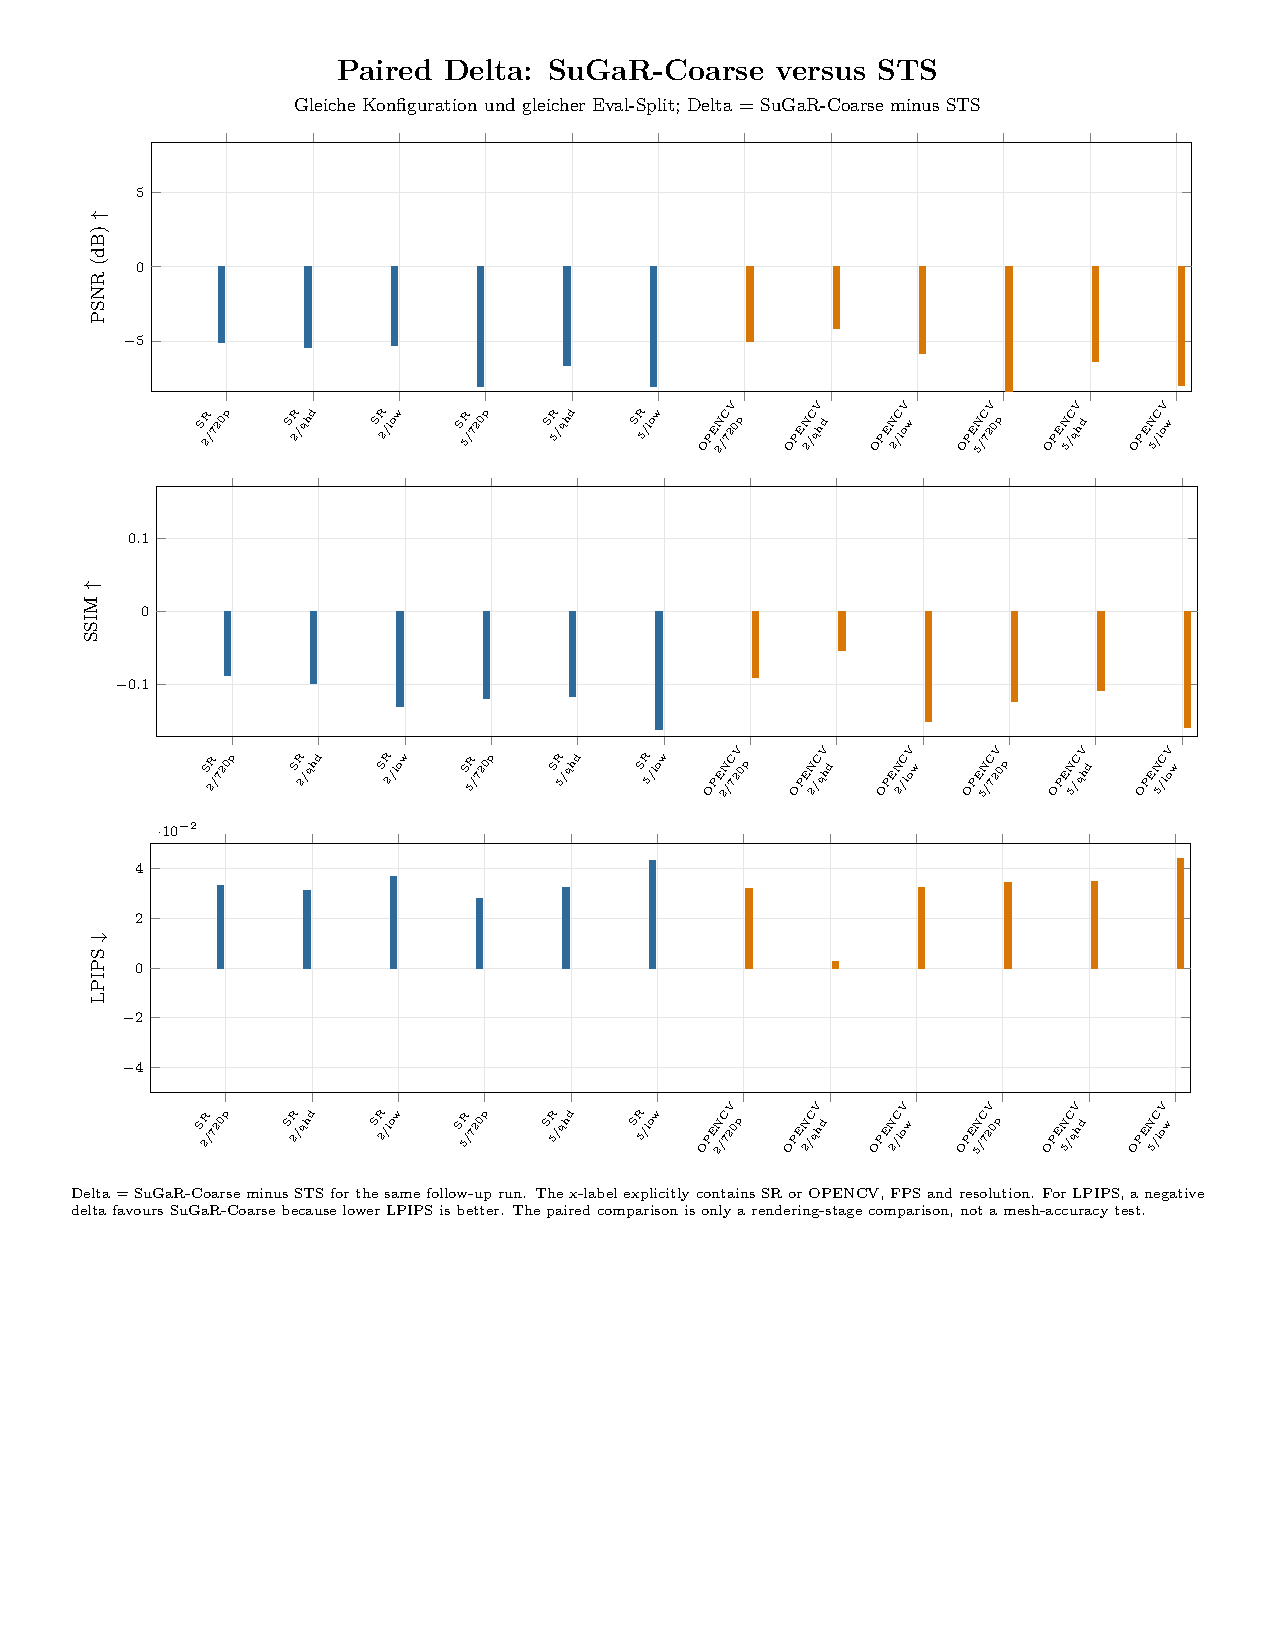
\includegraphics[width=\textwidth]{sugar_coarse_vs_sts_delta.pdf}
  \caption{Gepaarte Differenz zwischen SuGaR-Coarse und STS bei identischer
  Follow-up-Konfiguration. Negative PSNR-/SSIM-Werte und positive LPIPS-Werte
  bedeuten in diesen Läufen eine schlechtere SuGaR-Coarse-Bildmetrik; die
  Differenz ist kein Mesh-Genauigkeitsnachweis.}
  \label{fig:pa-sugar-delta}
\end{figure}

\begin{figure}[H]
  \centering
  
\includegraphics[width=\textwidth]{metric_vs_runtime.pdf}
  \caption{Explorative Beziehung zwischen objektmaskierten Bildmetriken und
  der archivierten Laufzeit der Pipeline-Segmente STS bis Postprocessing.
  SAM~3.1- und COLMAP-Wandzeit sind in diesen Segmentzeiten nicht enthalten;
  gemessene Gesamtlaufzeiten je Auflösung weist Abschnitt~\ref{sec:laufzeiten-e2e}
  separat aus.}
  \label{fig:pa-metric-runtime}
\end{figure}

In der Laufzeitgrafik ist die x-Achse auf 15--40 Minuten begrenzt und zeigt
die Gesamtlaufzeit des archivierten Pipeline-Laufs. Grün und Lila kodieren STS
und SuGaR-Coarse; kräftige und blasse Farbtöne kodieren 5 beziehungsweise
2 FPS. Kreis, Quadrat und Dreieck stehen für 720p, qHD und Low. Die Kamera
wird über die Achsenbeschriftung angegeben, nicht über eine zusätzliche
SR-/OPENCV-Legende.

\subsection{Funktionsnachweis der Endstufen}

Die erfolgreichen A-Läufe erzeugten neben den STS-Metriken auch Coarse-Ply,
kompatibles OBJ, lokale Centerline, B-Spline und GeoJSON. Die Georeferenzierung
war in den Matrixarchiven mangels validierter CloudCompare-Matrix teilweise ein
Translation-Fallback. Damit ist die technische Kette bis zu lokalen
Geometrieprodukten nachgewiesen; eine globale Genauigkeit ist daraus nicht
ableitbar.

Abbildung~\ref{fig:pa-panel-alurohr} zeigt das für den Testdatensatz erzeugte
Rohrmesh und die daraus abgeleitete lokale Centerline als Ergebnis der
Endstufen.

\begin{figure}[H]
  \centering
  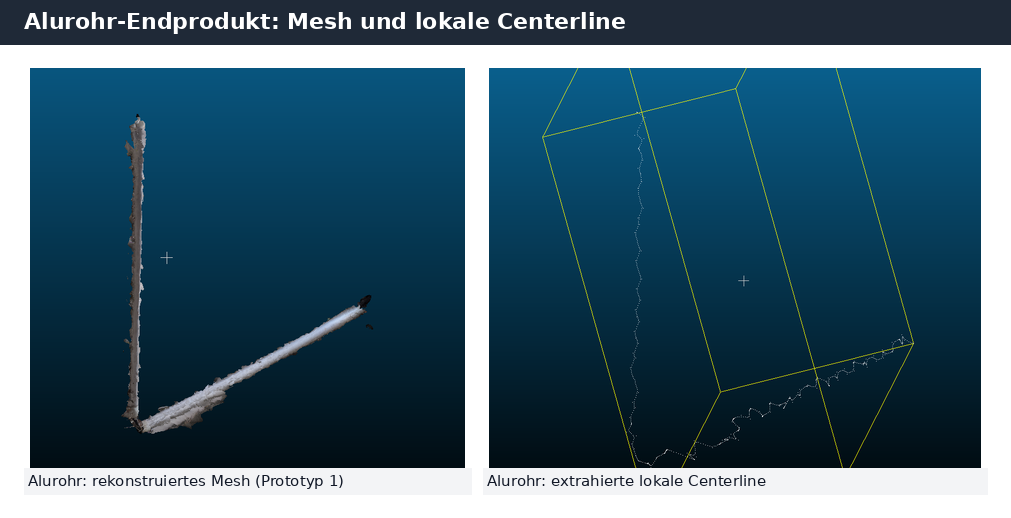
\includegraphics[width=\textwidth]{pa_panel_alurohr_endprodukt.png}
  \caption{Alurohr-Endprodukt: rekonstruiertes Rohrmesh und die daraus
  extrahierte lokale Centerline. Beide Ansichten stammen aus demselben
  Entwicklungsstand (18. Juli 2026).}
  \label{fig:pa-panel-alurohr}
\end{figure}

Beim kanonischen Produktionslauf (\path{Alurohr_THWS.mp4}, OPENCV, 5 FPS,
720p, Route~A) extrahierte DGtal 87 Rohpunkte; der
Grad-10-B-Spline erzeugte 380 Ausgabepunkte. Diese Zahlen belegen die
Ausführbarkeit des Postprocessings. Sie bewerten weder die Lage der Linie im
Rohr noch ihre Formabweichung gegen eine Referenz. Die anschaulichen
Centerline-Bilder der drei Auflösungsstufen finden sich in
Anhang~\ref{app:durchlauf}; dort sind sie als Teil der vollständigen
Durchlaufkette im Kontext der übrigen Zwischenstufen zu sehen.

\subsection{Negative Ergebnisse als Robustheitsbefund}

Mehrere zunächst fehlgeschlagene Läufe lieferten übertragbare Ergebnisse für
die Architektur. Die feste Eval-Liste muss Bildnamen unabhängig von
Dateiendungen abgleichen; die konkrete Eval-Maske muss nichtleer sein; ein
Unterprozess darf nicht die Konfigurations-TSV des Matrixrunners konsumieren;
und SuGaR-Renderings benötigen sowohl den richtigen Importpfad als auch das
erwartete Tensorlayout. Diese Korrekturen sind heute als Quality-Gates oder
explizite Fehlerprüfungen implementiert. Tabelle~\ref{tab:fehlerchronik}
dokumentiert weitere Fälle.

\section{Diskussion und Grenzen}

\subsection{Technische Machbarkeit und Robustheit}

Die Hauptfrage kann für den kontrollierten Alurohrdatensatz und den
nachgewiesenen Matrix-/Smoke-/Replaypfad grundsätzlich positiv beantwortet
werden. Die Verarbeitungskette kann aus einer Bildsequenz Masken und Kameras
erzeugen, objektbezogene Gaussians trainieren, ein Mesh ableiten und daraus
eine lokale Centerline samt B-Spline exportieren. Der wissenschaftlich
relevante Befund ist dabei nicht nur ein einzelner erfolgreicher Lauf. Die im
Matrix-/Replaypfad wirksamen Quality-Gates für Masken, Kameramodelle, ideale
Bilddomäne, Eval-Split und Ergebnisarchive verhindern mehrere zuvor
beobachtete stille oder verspätete Fehler; Inline-Vollauf, Matrixrunner und
Replays mit frischem COLMAP nutzen dieselbe Gate-/Warp-Kette, während
Replays ab \texttt{sts} einen bereits passenden idealen Maskensatz voraussetzen.

Robustheit bedeutet in dieser Arbeit nicht Fehlerfreiheit unter jeder
denkbaren Eingabe. Sie bedeutet, dass bekannte Voraussetzungen geprüft,
unvollständige Routen eindeutig markiert, teure Stufen an kontrollierten
Grenzen wiederholt und Ergebnisse reproduzierbar archiviert werden. Die
Untersuchung nur eines Testvideos begrenzt weiterhin die externe Validität.

\subsection{Masken, Domänen und Geometrie}

Die zentrale Domänentrennung löst einen methodischen Widerspruch: SfM profitiert
von unmaskierten Hintergrundmerkmalen, während STS und objektmaskierte
Metriken eine semantisch begrenzte ideale Bilddomäne benötigen. Die gemeinsame
Transformation von Bildern, Kameras und Masken stellt diese Konsistenz her.

Masken sind dennoch keine geometrische Referenz. Sie gewichten oder selektieren
Bildpixel und Objektzuordnungen. Position, Skalierung und Orientierung der
Gaussians, Kamerafehler, Surface-Sampling und Poisson-Rekonstruktion können die
3D-Geometrie weiterhin verändern. Deshalb ist die zunächst plausible Aussage,
eine niedrige Auflösung genüge bei korrekten Masken und registriertem COLMAP,
nur als technische Hypothese zulässig. Für einen erfolgreichen Lauf müssen alle
Datenverträge gelten; für geometrische Genauigkeit wäre zusätzlich eine
unabhängige Referenz notwendig.

\subsection{Kameramodell, FPS und Auflösung}

Die Matrix zeigt, dass Kameramodell, zeitliche Samplingdichte und Auflösung
nicht isoliert interpretiert werden dürfen. Die 2-FPS-Profile enthalten weniger
zeitlich benachbarte Ansichten; bei dünnen Objekten kann dies die SAM-
Propagation und die verfügbare Überdeckung erschweren. Die Maskensegmentierung
selbst war im Testdatensatz stabil: Das Rohr wurde über alle Auflösungen und
FPS-Profile hinweg in jedem Frame erkannt; instabil waren allenfalls die
numerischen Metrikwerte über die Konfigurationen hinweg (dort besteht keine
monotone Beziehung zu FPS oder Auflösung, siehe
Abschnitt~\ref{sec:visueller-aufloesungsvergleich}).

Die nativen Bildmetriken werden in unterschiedlichen Pixelräumen berechnet.
Downsampling wirkt dabei wie ein Tiefpassfilter: Feine Hochfrequenzfehler wie
Metallreflexionen oder feine Kantenverschiebungen werden beim Herunterrechnen
weggeglättet, sodass Low-Auflösung künstlich höhere Werte erreichen kann. Für
BIM und Vermessung ist 720p trotzdem überlegen: Die Objektdetailgröße pro
Pixel ist in 720p deutlich feiner als in low, sodass kleine Strukturmerkmale
des Rohrs erhalten bleiben, die im low-Bild unterschritten werden. Eine echte
GSD-Aussage wäre erst mit einer Maßstabsreferenz zulässig. Die Konsequenz ist
zweifach: Auflösungen dürfen nicht in einer globalen Rangliste verglichen
werden; belastbar sind nur gepaarte Vergleiche von STS gegen SuGaR innerhalb
derselben Auflösung. Ein strengerer
Auflösungsvergleich müsste alle Renderings auf eine gemeinsame Zielauflösung
und identische Eval-Views bringen. Die derzeitige Matrix ist deshalb ein
Engineering-Screening.

Wissenschaftlich belastbar sind deshalb nur gepaarte Vergleiche innerhalb
derselben Auflösungs-, Kameramodell- und FPS-Konfiguration. Die Boxplot-
Auswertung ergänzt die Mittelwerte um die Streuung der einzelnen Testansichten;
sie ersetzt aber nicht die geometrische Referenzmessung.

Die Bildtafeln des Pipeline-Durchlaufs in
Anhang~\ref{app:durchlauf} präzisieren diese Einschränkung: Trotz des gleichen
SIFT-Merkmalslimits sind in den Punktwolken kaum Auflösungsunterschiede
sichtbar; die sichtbaren Floater-, Rand- und Centerline-Unterschiede zeigen
jedoch, warum Bildmetrik und Geometrie getrennt bewertet werden müssen.

Der direkte PINHOLE-Lauf ist eine Ablation und kein Nachweis einer gelungenen
Entzerrung: Er erzwingt auf den Rohbildern die Annahme einer idealen Kamera,
während der Produktionsweg mit \texttt{OPENCV} zunächst Verzeichnung schätzt
und daraus eine separate ideale Szene erzeugt
(Abschnitt~\ref{sec:produktionskonfiguration}). Die von COLMAP ausgegebenen
Verzeichnungskoeffizienten sind geschätzte Parameter, keine gemessenen
Objektivdaten; der Reprojektionsfehler belegt interne Konsistenz, nicht die
physikalische Richtigkeit der Entzerrung. Für einen Vermessungsnachweis wäre
eine externe Kamerakalibrierung erforderlich; diese liegt nicht vor.

\subsection{Original-GS und SuGaR-Coarse}

Die Vierfeld-Ablation zeigt, dass nicht nur die verwendete Tiefenroute, sondern
auch die zusätzliche SuGaR-Coarse-Optimierung die resultierende Oberfläche
verändert. Route A bewahrt den STS-Zustand am direktesten und ist für das Ziel
einer stabilen Centerline deshalb der plausibelste Produktionsstandard. Mehr
Vertices oder sichtbar feinere Strukturen sind nicht automatisch besser, wenn
sie zugleich Spitzen oder veränderte Randstützen erzeugen.

Die Entscheidung ist bewusst vorläufig. Die Meshdistanzen vergleichen nur
Varianten untereinander. Sie geben keinen Abstand zum realen Alurohr an. Die
zwischenzeitlich abgeschlossene zwölfteilige SuGaR-Coarse-Folgematrix zeigt,
dass der reparierte Coarse-Renderpfad über beide Kameramodelle, drei
Auflösungen und zwei FPS-Profile technisch durchläuft. Sie liefert damit eine
deutlich breitere technische Evidenz als die frühere Einzelprüfung. Da in keinem
der zwölf Läufe ein `refined.ply` exportiert wurde, ist die Aussage weiterhin
auf SuGaR-Coarse beschränkt; eine SuGaR-Refined-Auswertung bleibt offen.

Der gepaarte Delta-Vergleich der zwölf Follow-up-Konfigurationen ist deshalb
als Rendervergleich zu lesen: SuGaR-Coarse wird jeweils mit dem STS-Splat
derselben Konfiguration verglichen. Über alle zwölf gepaarten Konfigurationen
liegt die SuGaR-Coarse-Bildmetrik durchgängig unter der STS-Baseline. Diese
konsistente Richtung ist eine zulässige Aussage der Delta-Grafik – SuGaR
schneidet in den Ansichtsmetriken durchgängig schlechter ab. Sie bleibt
allerdings ein Rendervergleich und kein Meshgenauigkeitsnachweis; die
Unterschiede können neben der zusätzlichen SuGaR-Optimierung auch aus dem
unterschiedlichen Renderpfad entstehen.

\subsection{Autopilot und Batchfähigkeit}

Der Matrixrunner belegt die serielle Batchverarbeitung deklarierter
Konfigurationen. Der Autopilot füllt interaktive Entscheidungen mit
Standardwerten und kann den manuellen GCP-Breakpoint überspringen. Beide
Funktionen sind verwandt, aber nicht identisch.

Die nutzerseitige Autonomie ist durch archivierte Autopilot-Volläufe belegt
(Abschnitt~\ref{sec:versuchsaufbau}, Erfolgskriterium~6). Die
Containerisierung und die nichtinteraktive Matrix bereiten einen Serverbetrieb
vor; ein Deployment, Mehrbenutzerbetrieb und Betriebsmonitoring wurden nicht
evaluiert. Eine formale Usability-Messung wurde ebenfalls nicht durchgeführt;
im Sinne der Nutzerfreundlichkeit wurden durch Tests gewonnene Standardwerte
jedoch so gesetzt, dass dem Nutzer wiederkehrende Entscheidungen abgenommen
werden.

\subsection{Laufzeit und Effizienz}

Der Zeit-/Qualitätsquotient ist ebenfalls sekundär. Er kombiniert normalisierte
PSNR-, SSIM- und LPIPS-Werte mit gleichen Gewichten; bei LPIPS kehrt sich das
Ranking um, da hier niedrigere Werte besser sind – das ist die Natur der
Metrik, keine Inversion der Daten. Er verwendet
nur die archivierten STS-bis-Postprocess-Zeiten. SAM~3.1- und COLMAP-Zeit sowie
Container-Overheads der Rendering- und Metrikschritte sind nicht vollständig
enthalten. Vollständige End-to-End-Zeiten liegen zwischenzeitlich aus dem
Verifikationsbatch \path{matrix_e2e_verifikation_260826} vor
(Abschnitt~\ref{sec:laufzeiten-e2e}); sie ergänzen die Ressourcenplanung,
ändern aber nichts an der Segmentbasis des Quotienten. Für die
Bachelorarbeit müssen Rohmetriken und geometrische
Referenzmetriken höher gewichtet werden.

Die Effizienzanalyse ist trotzdem praktisch relevant: Ein automatischer
Screeninglauf kann ungeeignete Kombinationen aussortieren, bevor eine
hochaufgelöste Produktionsrechnung erfolgt. Die Zeit-/Qualitätsauswertung
dient damit als Screening-Hilfe, nicht als primäre wissenschaftliche
Rangliste.

\subsection{Centerline, Georeferenzierung und externer Geltungsbereich}

Die größte technische Restaufgabe ist die echte Georeferenzierung. Ein
Translation-Fallback prüft zwar die Ausführung, sagt aber nichts über Lage-
oder Höhengenauigkeit aus. Ebenso sind die Testdaten keine reale Rohr- oder
Kabeltrasse und enthalten keine unabhängige GNSS-Referenzkurve.

Auch die lokale Centerline ist bisher nur als erzeugtes Artefakt validiert,
nicht gegen eine geometrisch definierte Referenz wie die wahre Scheitelachse
des Rohrs. Centerline und Scheitelachse fallen nur bei einer idealen
Rekonstruktion zusammen; ihr Vergleich setzt eine unabhängige Vermessung
voraus. Der \texttt{single}-Modus ist für eine einzelne Trasse robust,
verwirft aber bewusst Netzwerktopologie. Das ist für den Untersuchungsgegenstand
gewollt: Die Bachelorarbeit untersucht bewusst lineare Objekte ohne
Ringschluss oder Abzweigungen; eine Übertragung auf verzweigte Netze würde
neue Referenzdaten und eigene Graphmetriken erfordern und ist nicht Teil des
Scopes.

Für die Bachelorarbeit folgen daraus vier priorisierte Schritte: reale
Aufnahmebedingungen, echte GCP-/GNSS-Daten, validierte relative
4x4-Transformation sowie RMSE- und Hausdorff-Distanz einer extrahierten
Centerline gegen eine unabhängige Referenzkurve. Erst damit kann die
ingenieurtechnische Toleranz geprüft werden.

\subsection{Beantwortung der Forschungsfragen}

\begin{enumerate}
  \item Die konsistente Übergabe erfordert ein erhaltenes Originalmodell, eine
	  getrennte ideale Bilddomäne, denselben Warp für Masken, einen
	  nichtleeren gematchten Eval-Split und explizite Statusprüfungen aller
	  Ergebnisstufen.
  \item Kameramodell, FPS und Auflösung verändern die Ansichtsmetriken in
	  unterschiedlichen Richtungen: Kein Faktor führt über alle Konfigurationen
	  hinweg zu durchgängig besseren Werten (keine monotone Beziehung zwischen
	  Metrikwert und Faktorstufe). Die Maskensegmentierung selbst war dagegen
	  stabil – im Testvideo wurde das Rohr in jedem Frame erkannt. Die Matrix
	  erlaubt damit ein Screening, aber keinen isolierten Kausal- oder
	  Geometrienachweis.
  \item Route A bewahrt die Original-STS-Gaussians direkter und zeigt im
	  relativen Vergleich weniger unerwünschte Oberflächenveränderung. Ihre
	  absolute geometrische Richtigkeit bleibt offen.
  \item Der normale Inline-Vollauf und der Matrixrunner sind als
	  reproduzierbare Ausführungswege durch archivierte Läufe nachgewiesen
	  (Abschnitt~\ref{sec:versuchsaufbau}); der Autopilot ist über sechs
	  archivierte Volläufe belegt.
\end{enumerate}

\section{Fazit und Ausblick}

Die Projektarbeit zeigt für den kontrollierten Alurohrdatensatz die technische
Machbarkeit einer Docker-basierten Scan-to-BIM-Pipeline. SAM~3.1, unmaskiertes
COLMAP-SfM, ideale Bilddomäne, objektspezifisches STS, Original-GS-
Meshgewinnung und DGtal-Centerline können im normalen Inline-Vollauf und im
Matrixbetrieb als reproduzierbare Kette betrieben und archiviert werden. Der
Inline-Vollauf führt den Maskenwarp und die zugehörige Coverage-Prüfung
ebenfalls vor STS aus. Dies ist durch die archivierten Autopilot-Vollläufe
nachgewiesen (Abschnitt~\ref{sec:versuchsaufbau}).

Der Eigenbeitrag besteht insbesondere in der kameramodellbewussten Trennung von
Roh- und Idealbilddomäne, der konsistenten Nutzung der SAM-Masken, den
prüfbaren Datenverträgen zwischen fünf Containerumgebungen, der direkten
Original-GS-Meshroute sowie der automatisierten Versuchs- und
Fehlerauswertung. Interaktiver CLI-Betrieb, Autopilot und Matrixrunner decken
Erstlauf, Standardlauf und Batchverarbeitung ab.

Variante A ist für den Projektstand die bevorzugte Meshroute, weil sie die
STS-Gaussian-Geometrie direkter erhält als eine zusätzliche SuGaR-Coarse-
Optimierung. PINHOLE und OPENCV sind als Kameramodell-Ablationen technisch
vergleichbar. SuGaR-Coarse bleibt eine wichtige Vergleichsroute.

Die Ergebnisse liefern einen Funktionsnachweis, aber keinen
Vermessungsnachweis. Die Bachelorarbeit muss deshalb reale Aufnahmen,
geeignete GCP-/GNSS-Messungen, echte 4x4-Georeferenzierung und geometrische
Fehlermetriken ergänzen. Die in dieser Arbeit aufgebaute Struktur trennt diese
wissenschaftlichen Fragen von den bereits geprüften technischen
Zwischenschritten. Insbesondere sind die von COLMAP geschätzten
Kameraverzeichnungsparameter ohne unabhängige Checkerboard- oder
ChArUco-Kalibrierung nicht als physikalisch validierte Objektivdaten zu
interpretieren.


% Literatur vor dem Anhangsteil (Zielrahmen §3); LoF/LoT bleiben vorne (D4 offen).
\printbibliography[heading=bibintoc,title={Literatur und Referenzen}]

\ifincludeappendices
\appendix
\section{Anhang: COLMAP-Vorstudie}

Die COLMAP-Voruntersuchung wurde als separater Benchmark mit COLMAP
\parencite{colmapProject} durchgeführt und ist
nicht mit der späteren GPU-Gesamtpipeline gleichzusetzen. Sie bewertet nur die
Sparse-SfM-Stufe auf dem Alurohr-Testdatensatz.

\begin{table}[H]
\centering
\small
\begin{tabularx}{\textwidth}{Xrrrrr}
\toprule
Konfiguration & Punkte & Punkte/Bild & Tracks & Reprojektion & Zeit (s)\\
\midrule
Plain-SIFT 4096 & 139.449 & 581 & 6,69 & 0,693 Pixel & 876\\
Plain-SIFT 4096 + Guided & 142.208 & 593 & 7,44 & 0,790 Pixel & 1.678\\
Plain-SIFT 8192 & 140.594 & 586 & 6,71 & 0,698 Pixel & 925\\
CRF 18 & 94.616 & 394 & 6,64 & 0,728 Pixel & 677\\
CRF 28 & 93.703 & 390 & 6,43 & 0,761 Pixel & 725\\
\bottomrule
\end{tabularx}
\caption{Optionale COLMAP-SfM-Voruntersuchung. Die Läufe sind ein separater
Benchmark und kein vollständiger STS-/SuGaR-Vergleich.}
\label{tab:colmap-vorstudie}
\end{table}

Die Ergebnisse begründen den Projektarbeitsstandard Plain-SIFT mit 4096
Merkmalen, Sequential-Overlap 15 und deaktiviertem Guided Matching. Guided
Matching brachte nur einen kleinen Punktezuwachs, erhöhte jedoch die Laufzeit
stark und verschlechterte den mittleren Reprojektionsfehler. Die vollständigen
Rohberichte liegen im digitalen Anlagenband unter \path{02_COLMAP_Tests/}
(siehe \texttt{ABGABE\_Index.md}).

\section{Optionaler Anhang: Matrix- und Robustheitstests}

Die Matrix ist ein kontrollierter Screening-Versuch, kein vollständiger
Vermessungsnachweis. Die historische STS-Auswertung umfasst den Batch
\texttt{matrix\_full\_pipe} und den Folge-Batch \texttt{matrix\_rest}
\parencite{matrixRestResults}. Die
sechs A-Läufe des ersten Batches werden als bereits ausgeführte Referenz
markiert; im Folge-Batch wurden PINHOLE und OPENCV als Original-GS-Ablationen
bei 2 und 5 FPS sowie drei Auflösungen getestet. Die SuGaR-Coarse-Auswertung
steht als separate, inzwischen abgeschlossene Folgematrix
\texttt{matrix\_sugar\_followup\_12} daneben.

\begin{table}[H]
\centering
\small
\begin{tabular}{lrrr}
\toprule
Batch & Versuche & vollständig erfolgreich & unvollständig\\
\midrule
matrix\_full\_pipe & 6 & 4 & 2\\
matrix\_rest & 18 & 12 & 6\\
Gesamt & 24 & 16 & 8\\
\bottomrule
\end{tabular}
\caption{Status der für die PA zusammengeführten Matrixbatches.}
\end{table}

Die sechs historischen SuGaR-Coarse-Läufe des Batches
\texttt{matrix\_rest} besitzen teilweise eine STS-Baseline-Metrik, sind aber
wegen des damaligen technischen Importfehlers im SuGaR-Render-Helfer nicht als
erfolgreiche SuGaR-Ergebnisse zu werten. Die Statusauswertung trennt daher
technische Vollständigkeit und vorhandene Zwischenmetriken. Die vollständige
STS-Übersicht liegt in
\path{docs/grafiken/matrix_repeat_2026-08-17/sts_masked_overview.pdf};
die getrennte SuGaR-Coarse-Übersicht liegt in
\path{docs/grafiken/matrix_repeat_2026-08-17/sugar_coarse_masked_overview.pdf}.
Die gemeinsame historische CSV-Quelle liegt in
\path{docs/grafiken/verwendet_verbessert/matrix_thesis_data.csv}; die neue
stufenspezifische Auswertung schreibt zusätzlich
\path{docs/grafiken/matrix_repeat_2026-08-17/sts_masked_summary.csv} und
\path{docs/grafiken/matrix_repeat_2026-08-17/sugar_coarse_masked_summary.csv}.

\subsection*{Abgeschlossene SuGaR-Coarse-Folgematrix}

Die Repeat-Konfiguration \path{tools/experiment_matrix_repeat.tsv} enthält für
SuGaR-Coarse zwölf Läufe: \path{SIMPLE_RADIAL/sugar_coarse} und
\path{OPENCV/sugar_coarse} bei drei Auflösungen und zwei FPS-Profilen. Der
Render-Helfer wurde vor dieser Prüfung durch einen expliziten
\texttt{/opt/sugar}-Importpfad und eine HWC-zu-CHW-Konvertierung korrigiert.
Ein archivierter 5-FPS-720p-Checkpoint ließ sich damit bereits auf 30
Testansichten rendern und objektmaskiert auswerten.

Die zwölf SuGaR-Coarse-Läufe unter \path{data/10_runs/matrix_repeat_20260812/}
sind abgeschlossen. Alle zwölf Manifeste tragen den Status \texttt{success}.
Die Coarse-Meshgewinnung, das SuGaR-Coarse-Rendering, die objektmaskierte
Metrikberechnung und das Postprocessing wurden für beide Kameramodelle sowie
alle Auflösungs-/FPS-Kombinationen erfolgreich archiviert. Die
\texttt{sugar\_refined\_masked.json}-Dateien weisen dagegen ausdrücklich
\texttt{no refined.ply exported} aus; die Folgematrix ist daher ein
SuGaR-Coarse-Nachweis und kein vollständiger SuGaR-Refinement-Vergleich.

\begin{table}[H]
\centering
\small
\begin{tabularx}{\textwidth}{l l rrr}
\toprule
Kameramodell & Auflösung & PSNR$\uparrow$ & SSIM$\uparrow$ & LPIPS$\downarrow$\\
\midrule
SIMPLE\_RADIAL & 720p & 21,43 & 0,766 & 0,153\\
SIMPLE\_RADIAL & qHD  & 21,59 & 0,757 & 0,140\\
SIMPLE\_RADIAL & Low  & 21,87 & 0,752 & 0,125\\
OPENCV         & 720p & 21,38 & 0,761 & 0,154\\
OPENCV         & qHD  & 21,60 & 0,754 & 0,144\\
OPENCV         & Low  & 21,84 & 0,747 & 0,126\\
\bottomrule
\end{tabularx}
\caption{SuGaR-Coarse-Mittelwerte aus 2 und 5 FPS des Repeat-Batches. Die
Werte sind objektmaskierte Ansichtsmetriken und kein
Geometrienachweis.}
\label{tab:sugar-followup-average}
\end{table}

Die vollständigen Einzelwerte und die getrennten Darstellungen für Status,
PSNR, SSIM, LPIPS und Zeit/Qualität liegen in den digitalen Anlagen unter
\path{docs/grafiken/matrix_repeat_2026-08-17/}. Alle zwölf Läufe verwendeten den
festen Eval-Split; bei 2 FPS wurden zwölf und bei 5 FPS dreißig gültige
Evaluationsansichten ausgewertet. Die Laufzeit-/Qualitätsgrafik nutzt die
archivierte vollständige Pipelinezeit und ist wie bei der STS-Matrix nur ein
sekundärer Screening-Index.

\clearpage
\begin{figure}[H]
\centering
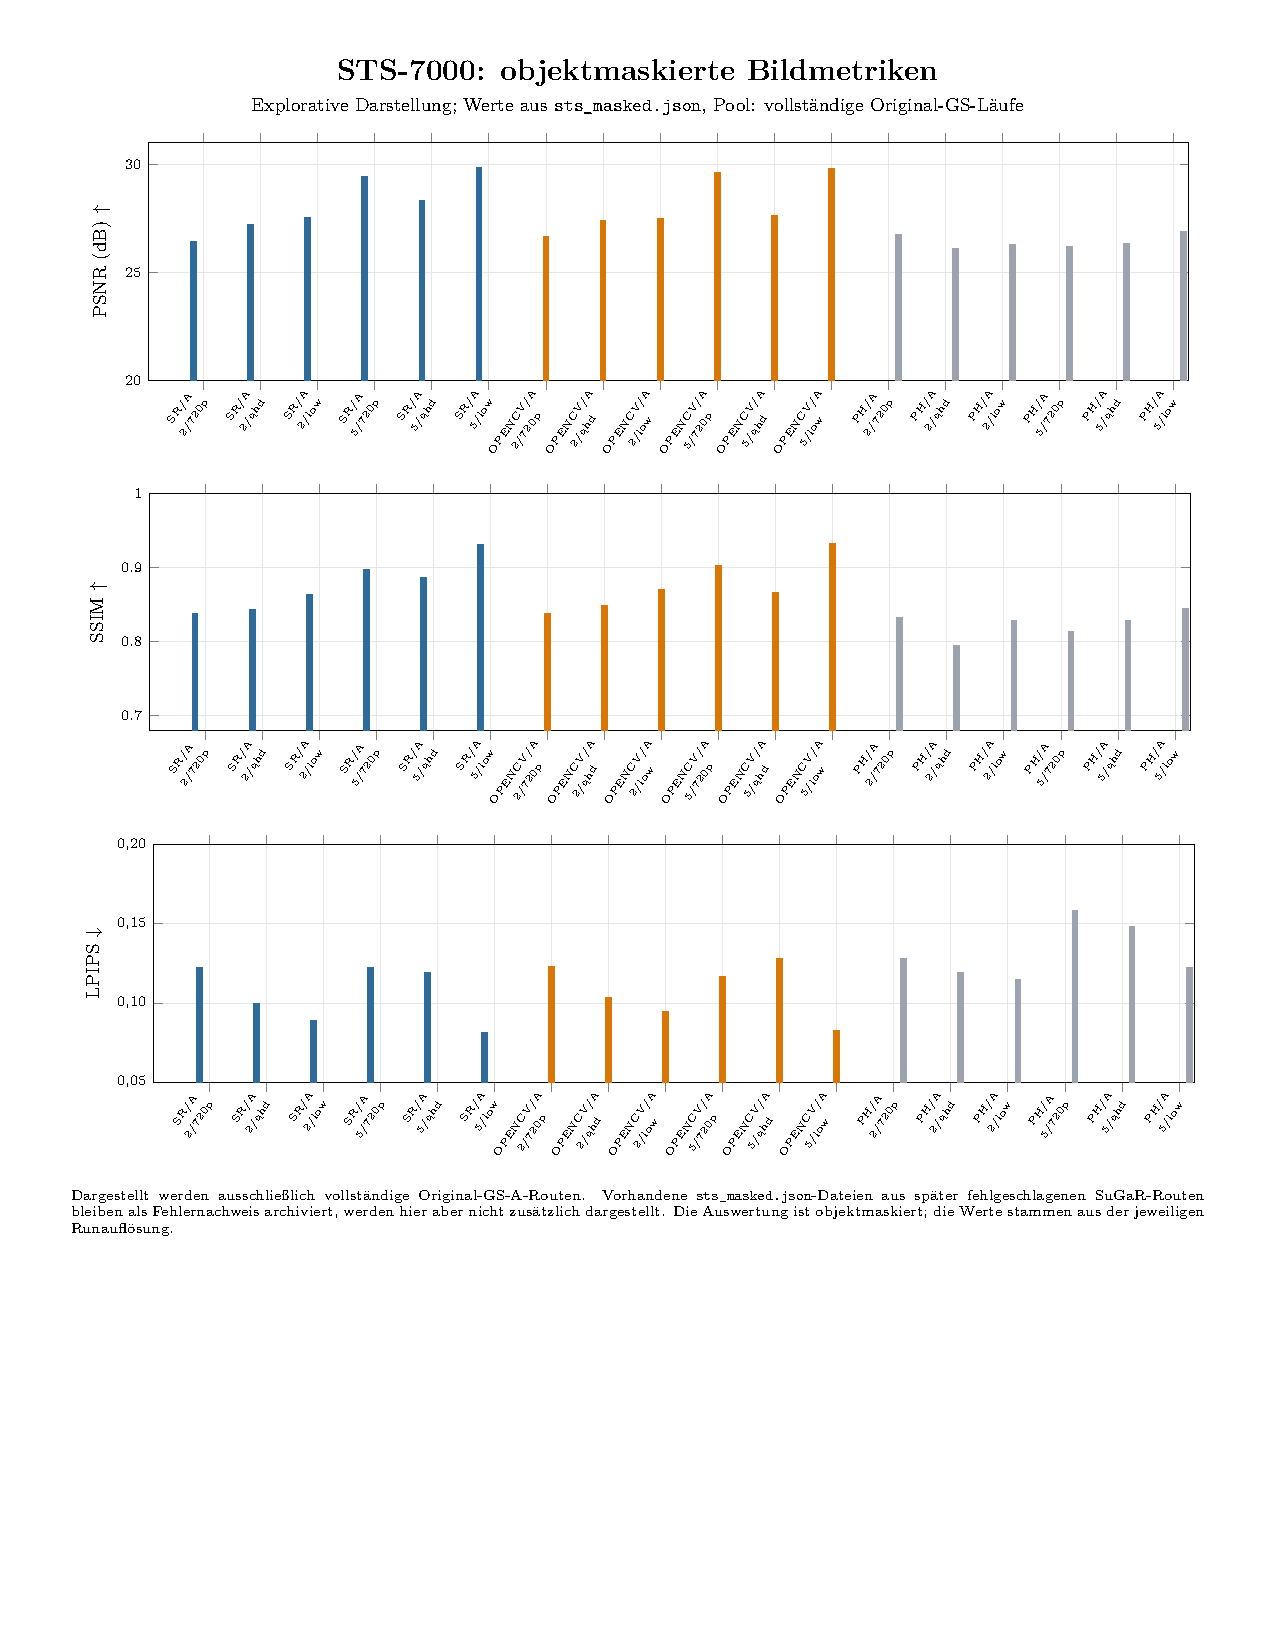
\includegraphics[width=\textwidth]{sts_masked_overview.pdf}
\caption{Objektmaskierte STS-Übersicht der vollständigen Original-GS-Route A.}
\end{figure}

\clearpage
\begin{figure}[H]
\centering
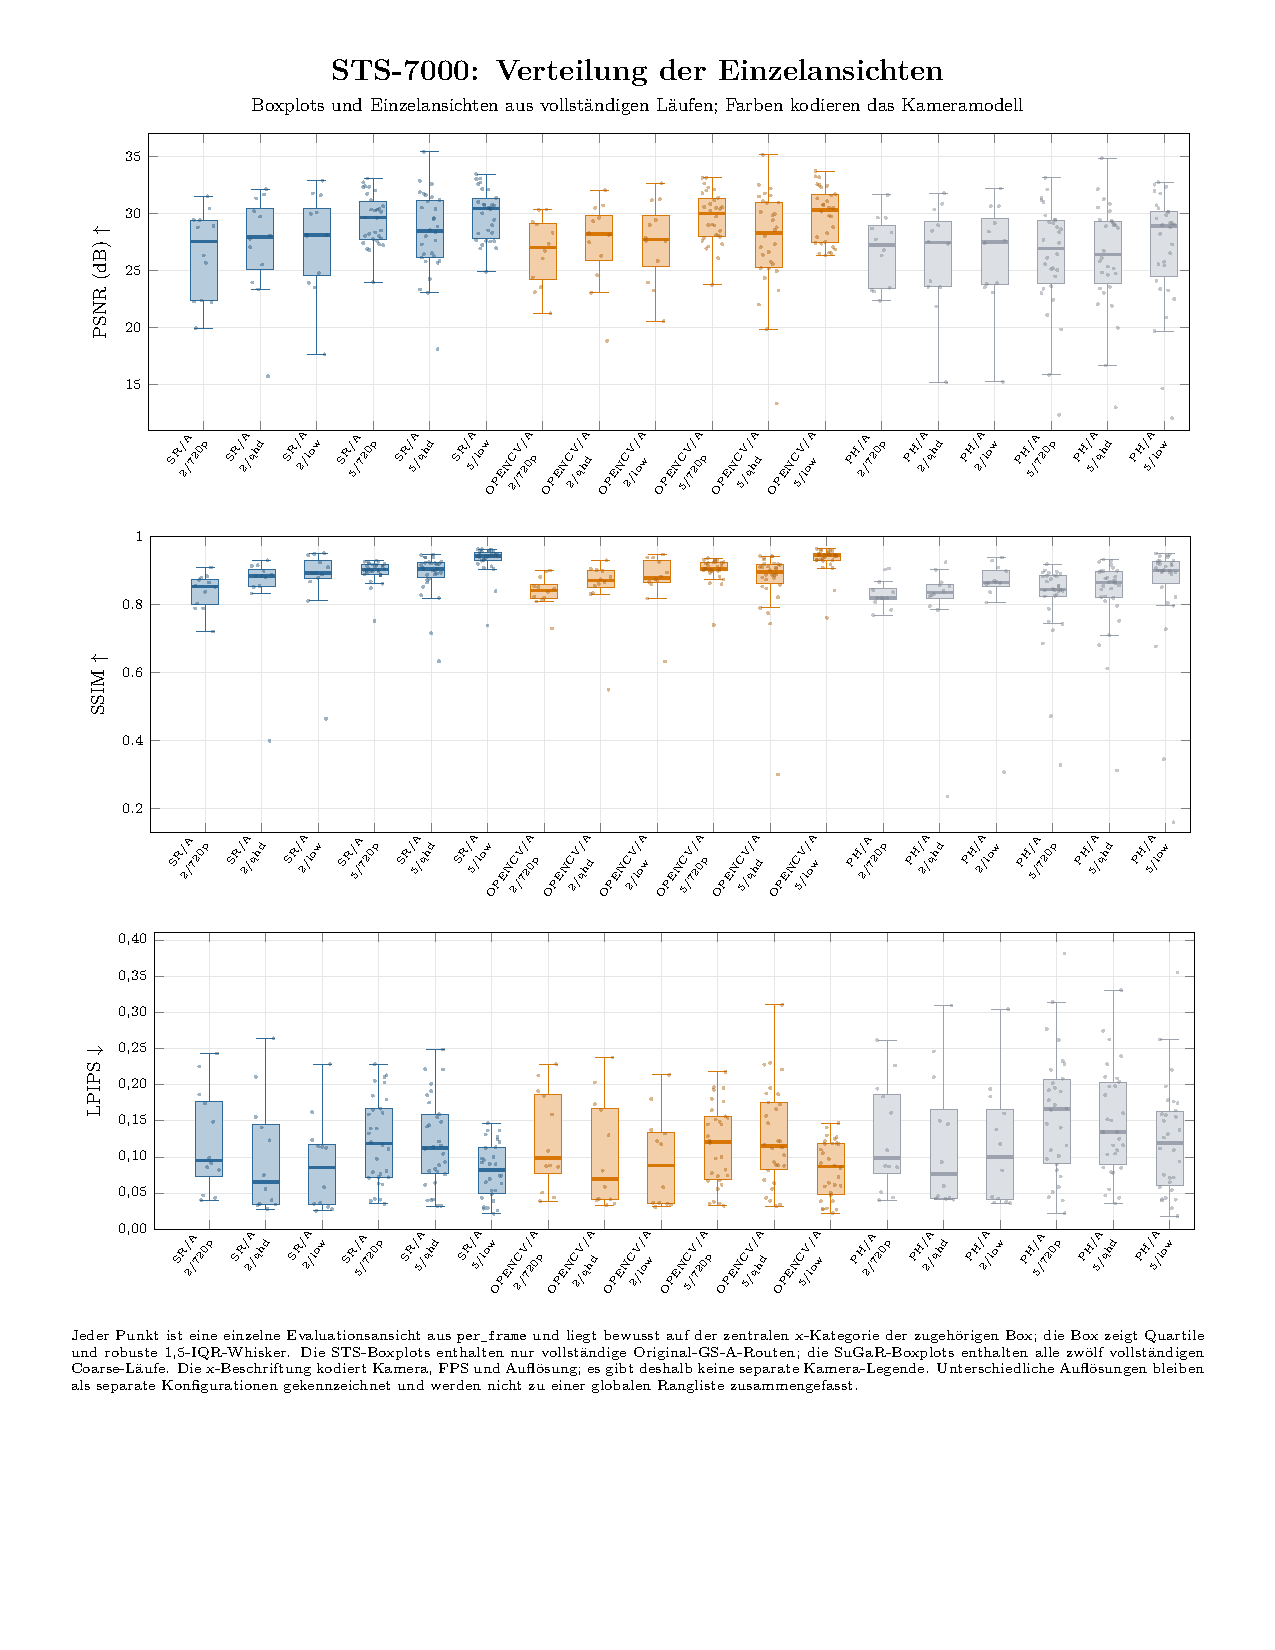
\includegraphics[width=\textwidth]{sts_masked_per_frame_boxplots.pdf}
\caption{Boxplots und Einzelansichten der STS-Route-A-Metriken.}
\end{figure}

\clearpage
\begin{figure}[H]
\centering

\includegraphics[width=\textwidth]{sugar_coarse_masked_overview.pdf}
\caption{Objektmaskierte SuGaR-Coarse-Übersicht mit PSNR, SSIM und LPIPS.}
\end{figure}

\clearpage
\begin{figure}[H]
\centering
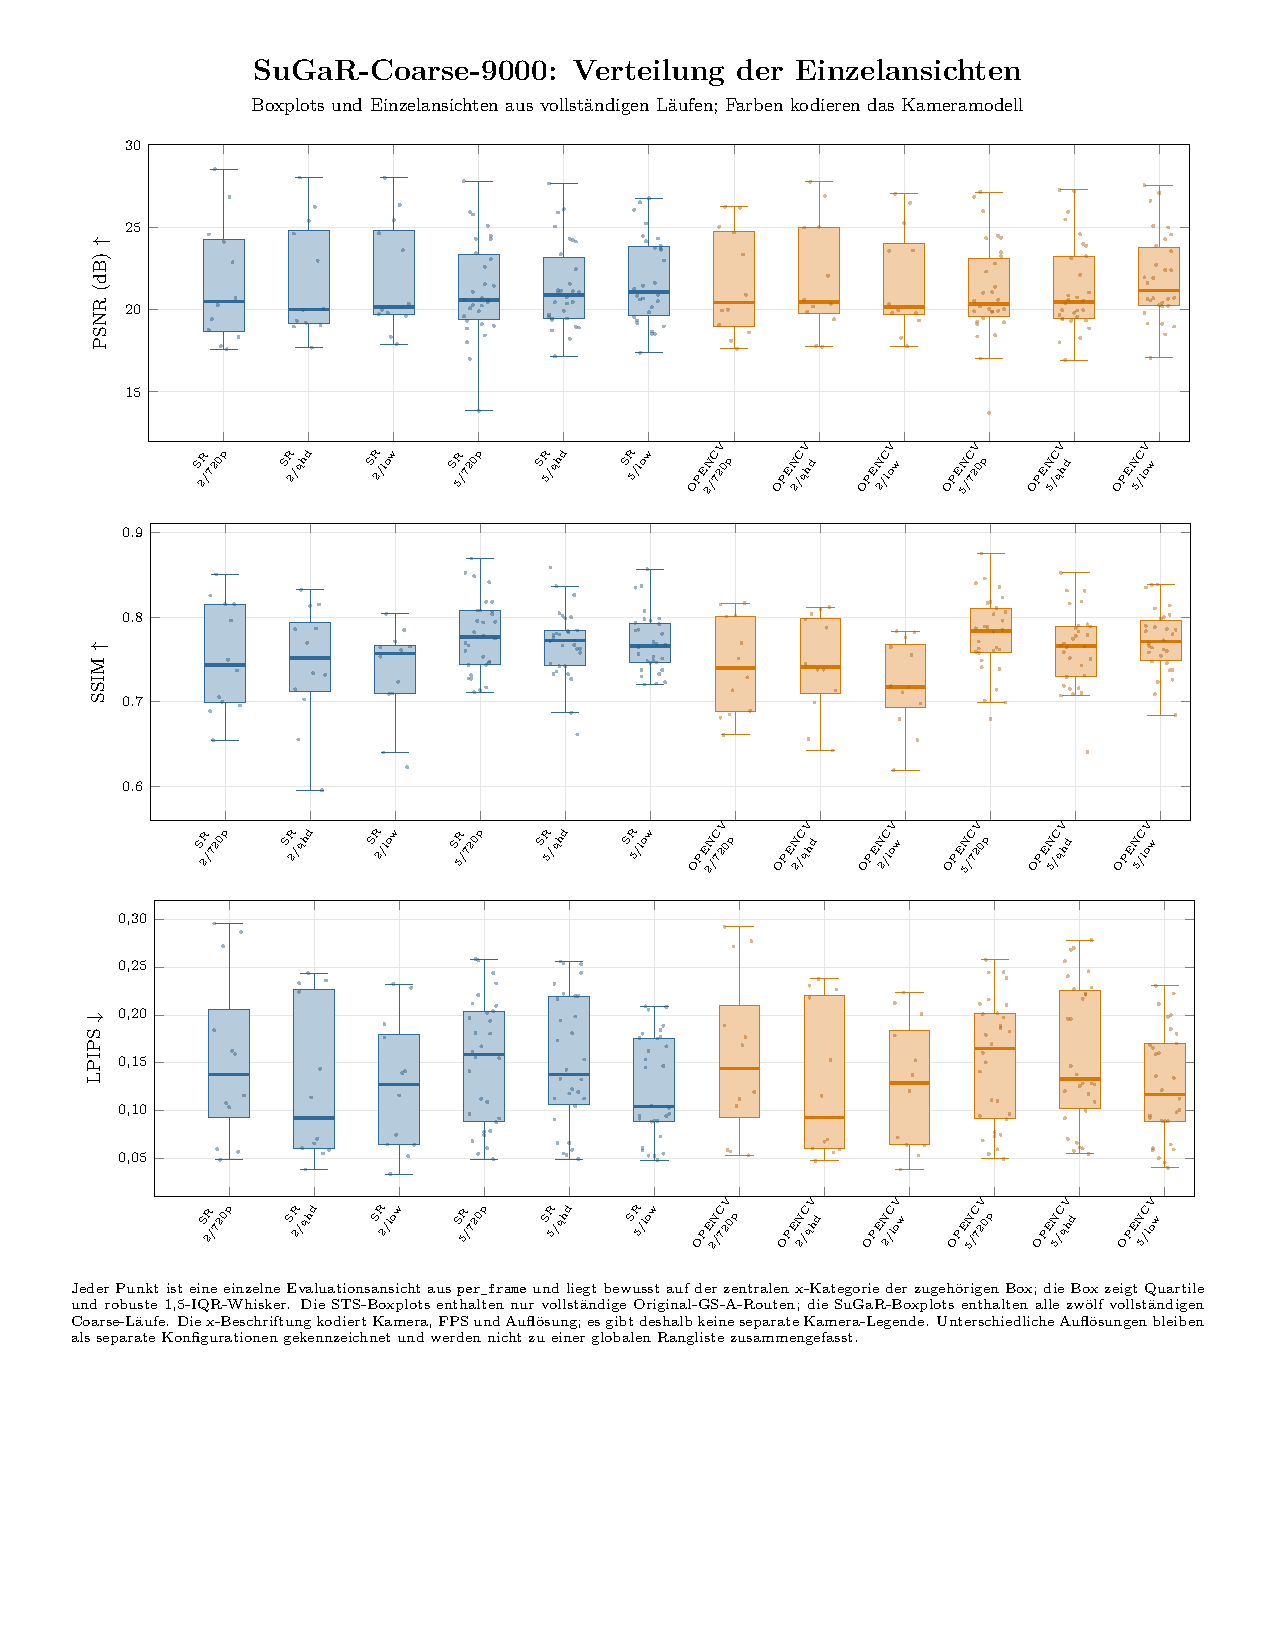
\includegraphics[width=\textwidth]{sugar_coarse_masked_per_frame_boxplots.pdf}
\caption{Boxplots und Einzelansichten der SuGaR-Coarse-Metriken.}
\end{figure}

\clearpage
\begin{figure}[H]
\centering
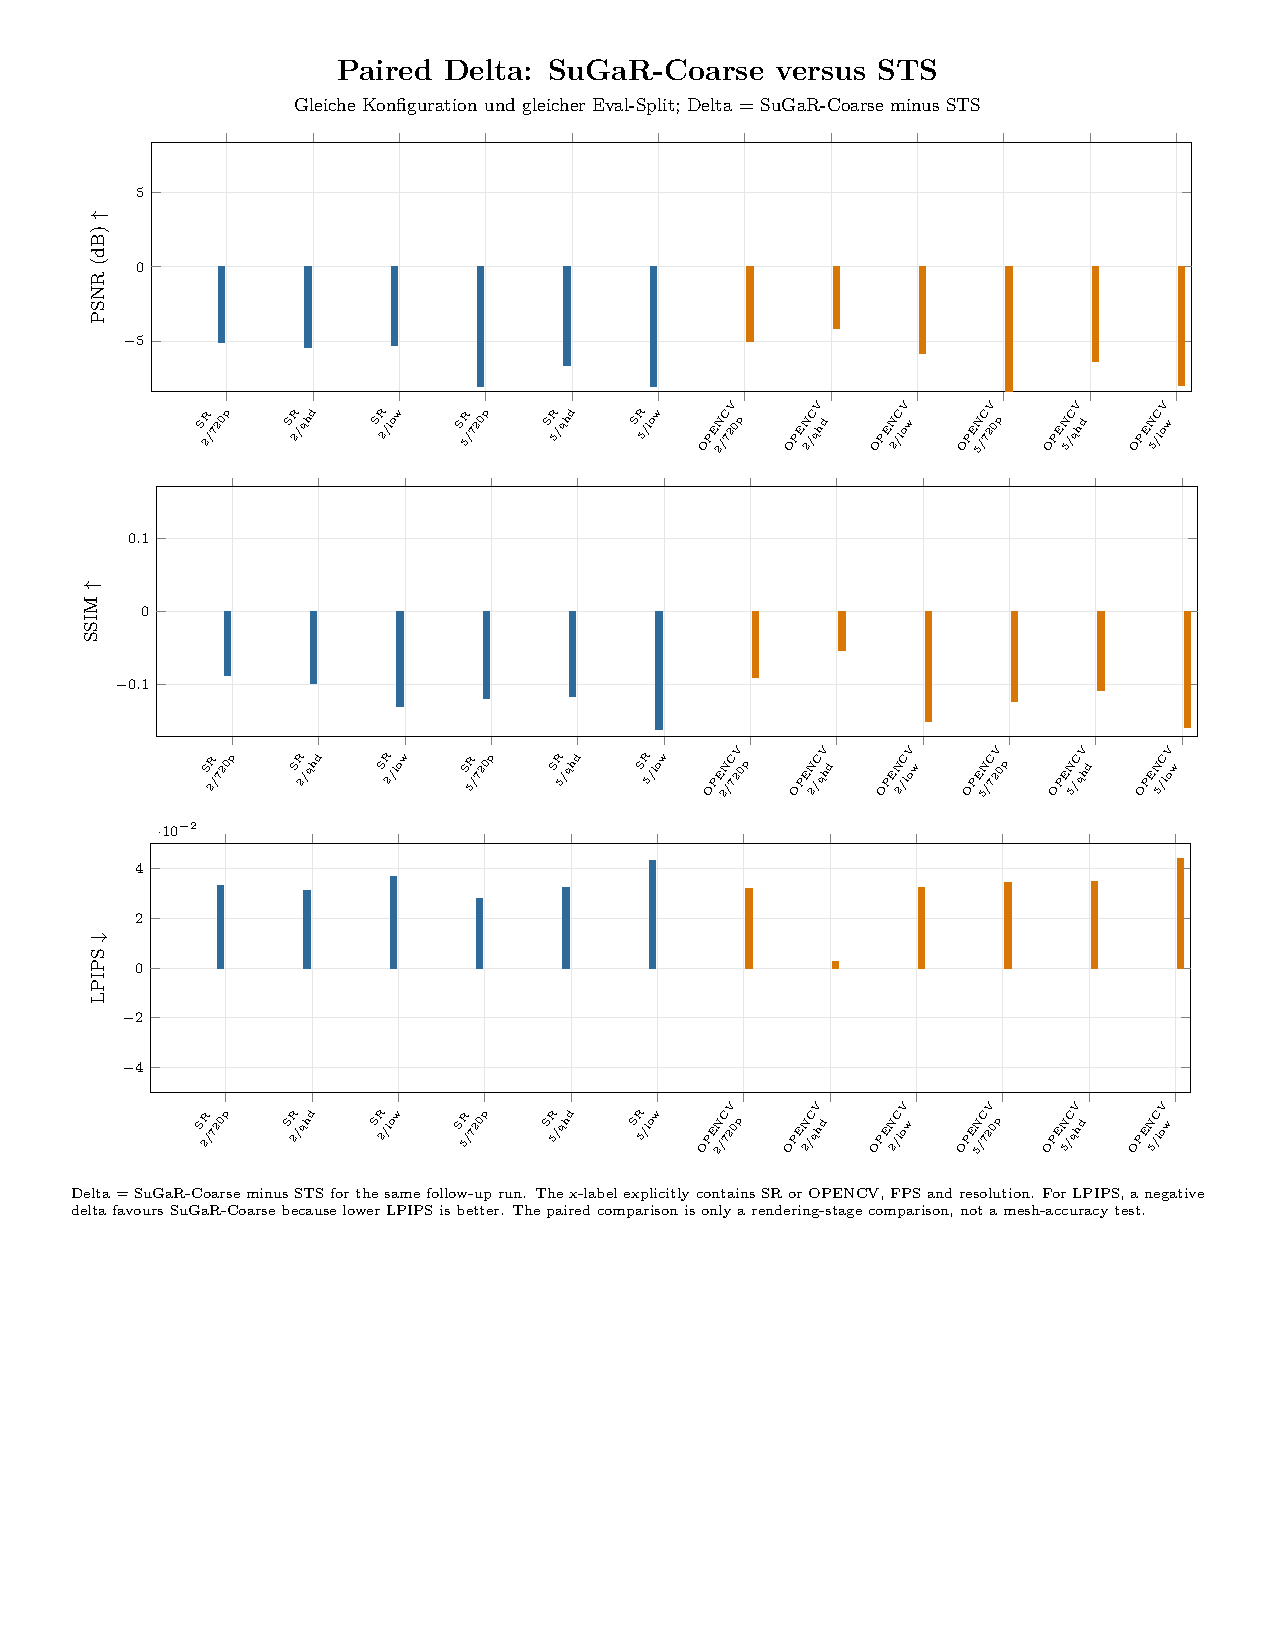
\includegraphics[width=\textwidth]{sugar_coarse_vs_sts_delta.pdf}
\caption{Gepaarte Differenz von SuGaR-Coarse und STS bei identischen
Konfigurationen.}
\end{figure}

\clearpage
\begin{figure}[H]
\centering

\includegraphics[width=\textwidth]{metric_vs_runtime.pdf}
\caption{Explorative Beziehung zwischen Bildmetriken und archivierter Laufzeit.}
\end{figure}

\clearpage
\subsection*{Regeln für die Auswertung}

\begin{itemize}
  \item \texttt{sts\_masked.json} ist die STS-Baseline vor dem separaten
	  SuGaR-Rendering und kein SuGaR-Ergebnis.
  \item Ein Average wird nur gebildet, wenn 2-FPS- und 5-FPS-Lauf derselben
	  Konfiguration vollständig erfolgreich sind.
  \item Fehlgeschlagene Läufe bleiben im Statusbericht und erhalten keinen
	  künstlich schlechten Metrikwert.
  \item Bildmetriken werden nur innerhalb nichtleerer Objektmasken berechnet.
  \item Native Auflösungen sind wegen Downsampling nicht unmittelbar als
	  Geometriequalität vergleichbar.
\end{itemize}

\clearpage
\section{Anhang: Pipeline-Durchlauf in drei Auflösungen}
\label{app:durchlauf}

Dieser Anhang zeigt die Zwischenstände eines vollständigen Pipeline-Durchlaufs
für drei Auflösungen desselben Testdatensatzes (5~FPS, OPENCV-Kameramodell).
Jede Zeile entspricht einer Zwischenstufe der Verarbeitung, jede Spalte einer
Auflösung: links \texttt{720p}, in der Mitte \texttt{qHD} und rechts
\texttt{low}. Die Reihenfolge folgt dem Datenfluss der Pipeline. Als Eingabe
dient das Videomaterial des Alurohr-Referenzdatensatzes. Über den Prompt
\texttt{pipe} wird das Zielobjekt promptbasiert segmentiert. Ab diesem
Schritt verzweigt der Pfad in die drei Spalten der Auflösungsvarianten.

% Die Querformatseiten erhalten eine eigene Satzvorlage. Dadurch werden die
% normalen, hochkant gesetzten fancyhdr-Kopf- und Fußzeilen unterdrückt.
\newcommand{\durchlaufheader}{%
  \vspace*{-59.5pt}%
  {\small
  \noindent Projektarbeit -- Scan-to-BIM-Pipeline\hfill Studienbereich Geo\par
  \vspace{2pt}\hrule height 0.4pt\vspace{6pt}}%
  \vspace{59.5pt}}
\newcommand{\durchlauffooter}{%
  \par\vspace*{\fill}%
  \begin{center}\small\thepage\end{center}%
  \vspace*{-41.2pt}}
\newcommand{\durchlaufbild}[1]{%
  \makebox[\hsize][c]{\includegraphics[width=0.95\hsize]{#1}}}
\newcommand{\durchlaufmasken}[1]{%
  \begin{minipage}[t]{\hsize}
  \centering
  
\includegraphics[width=0.95\linewidth]{Screenshots/Pipline_Durchlauf/#1/review_ideal/frame_00000_middle_panel.png}\par\vspace{1pt}%
  
\includegraphics[width=0.95\linewidth]{Screenshots/Pipline_Durchlauf/#1/review_ideal/frame_00080_middle_panel.png}\par\vspace{1pt}%
  
\includegraphics[width=0.95\linewidth]{Screenshots/Pipline_Durchlauf/#1/review_ideal/frame_00160_middle_panel.png}\par\vspace{1pt}%
  
\includegraphics[width=0.95\linewidth]{Screenshots/Pipline_Durchlauf/#1/review_ideal/frame_00239_middle_panel.png}%
  \end{minipage}}

\begin{landscape}
\thispagestyle{empty}
\durchlaufheader
\small
\renewcommand{\arraystretch}{1.05}
\setlength{\tabcolsep}{3pt}
\noindent
\begin{tabularx}{\linewidth}{@{}>{\raggedright\arraybackslash}p{2.4cm}>{\centering\arraybackslash}X>{\centering\arraybackslash}X>{\centering\arraybackslash}X@{}}
\toprule
Zwischenstufe & \textbf{\texttt{720p}} & \textbf{\texttt{qHD}} & \textbf{\texttt{low}}\\
\midrule
Masken (Prüfpanels) &
\durchlaufmasken{720p_Panels} &
\durchlaufmasken{qhd_panels} &
\durchlaufmasken{low_panels} \\
\bottomrule
\end{tabularx}
\par\vspace{3pt}
\noindent\parbox{\linewidth}{\footnotesize\textit{Maskenprüfung bei
\texttt{720p}, \texttt{qHD} und \texttt{low}. Je Auflösung sind die vier
Prüfzeitpunkte 00000, 00080, 00160 und 00239 untereinander dargestellt; jedes
Panel zeigt das Originalbild, die überlagerte \texttt{middle}-Maske und den
Objektausschnitt.}}
\durchlauffooter
\newpage

\thispagestyle{empty}
\durchlaufheader
\small
\renewcommand{\arraystretch}{1.05}
\setlength{\tabcolsep}{3pt}
\noindent
\begin{tabularx}{\linewidth}{@{}>{\raggedright\arraybackslash}p{2.4cm}>{\centering\arraybackslash}X>{\centering\arraybackslash}X>{\centering\arraybackslash}X@{}}
\toprule
Zwischenstufe & \textbf{\texttt{720p}} & \textbf{\texttt{qHD}} & \textbf{\texttt{low}}\\
\midrule
Punktwolken &
\durchlaufbild{Screenshots/Pipline_Durchlauf/Punktwolke_OpenCV_720p.png} &
\durchlaufbild{Screenshots/Pipline_Durchlauf/Punktwolke_OpenCV_qhd.png} &
\durchlaufbild{Screenshots/Pipline_Durchlauf/Punktwolke_OpenCV_low.png} \\
Punktwolken (Zoom) &
\durchlaufbild{Screenshots/Pipline_Durchlauf/Punktwolke_OpenCV_720p_zoom.png} &
\durchlaufbild{Screenshots/Pipline_Durchlauf/Punktwolke_OpenCV_qhd_zoom.png} &
\durchlaufbild{Screenshots/Pipline_Durchlauf/Punktwolke_OpenCV_low_zoom.png} \\
\bottomrule
\end{tabularx}
\par\vspace{3pt}
\noindent\parbox{\linewidth}{\footnotesize\textit{COLMAP-Punktwolken und vergrößerte Detailansichten
bei \texttt{720p}, \texttt{qHD} und \texttt{low}.}}
\durchlauffooter
\newpage

\thispagestyle{empty}
\durchlaufheader
\small
\renewcommand{\arraystretch}{1.05}
\setlength{\tabcolsep}{3pt}
\noindent
\begin{tabularx}{\linewidth}{@{}>{\raggedright\arraybackslash}p{2.4cm}>{\centering\arraybackslash}X>{\centering\arraybackslash}X>{\centering\arraybackslash}X@{}}
\toprule
Zwischenstufe & \textbf{\texttt{720p}} & \textbf{\texttt{qHD}} & \textbf{\texttt{low}}\\
\midrule
Splat (Opazität 9999) &
\durchlaufbild{Screenshots/Pipline_Durchlauf/Splat_OpenCV_720p_9999opac.png} &
\durchlaufbild{Screenshots/Pipline_Durchlauf/Splat_OpenCV_qhd_9999opac.png} &
\durchlaufbild{Screenshots/Pipline_Durchlauf/Splat_OpenCV_low_9999opac.png} \\
Mesh &
\durchlaufbild{Screenshots/Pipline_Durchlauf/Splats_to_Mesh_720p.png} &
\durchlaufbild{Screenshots/Pipline_Durchlauf/Splats_to_Mesh_qhd.png} &
\durchlaufbild{Screenshots/Pipline_Durchlauf/Splats_to_Mesh_low.png} \\
\bottomrule
\end{tabularx}
\par\vspace{3pt}
\noindent\parbox{\linewidth}{\footnotesize\textit{Splat- und Mesh-Zwischenstände bei
\texttt{720p}, \texttt{qHD} und \texttt{low}.}}
\durchlauffooter
\newpage

\thispagestyle{empty}
\durchlaufheader
\small
\renewcommand{\arraystretch}{1.05}
\setlength{\tabcolsep}{3pt}
\noindent
\begin{tabularx}{\linewidth}{@{}>{\raggedright\arraybackslash}p{2.4cm}>{\centering\arraybackslash}X>{\centering\arraybackslash}X>{\centering\arraybackslash}X@{}}
\toprule
Zwischenstufe & \textbf{\texttt{720p}} & \textbf{\texttt{qHD}} & \textbf{\texttt{low}}\\
\midrule
Mesh (ohne Nachbearbeitung) &
\durchlaufbild{Screenshots/Pipline_Durchlauf/Splats_to_Mesh_720p_ugly.png} &
\durchlaufbild{Screenshots/Pipline_Durchlauf/Splats_to_Mesh_qhd_ugly.png} &
\durchlaufbild{Screenshots/Pipline_Durchlauf/Splats_to_Mesh_low_ugly.png} \\
Centerline &
\durchlaufbild{Screenshots/Pipline_Durchlauf/Centerline_720p.png} &
\durchlaufbild{Screenshots/Pipline_Durchlauf/Centerline_qhd.png} &
\durchlaufbild{Screenshots/Pipline_Durchlauf/Centerline_low.png} \\
\bottomrule
\end{tabularx}
\par\vspace{3pt}
\noindent\parbox{\linewidth}{\footnotesize\textit{Unbearbeiteter Mesh-Rohstand und extrahiertes
Linienelement (Centerline) als Endstufen der Pipeline bei \texttt{720p},
\texttt{qHD} und \texttt{low}.}}
\durchlauffooter
\end{landscape}

\clearpage
\section{Entwicklungs- und Fehlerchronologie}

Dieser Anhang bewahrt wesentliche negative Ergebnisse und Korrekturen. Im
Haupttext werden nur die wissenschaftlich entscheidenden Datenverträge und
Schutzmaßnahmen erläutert.

\begin{table}[H]
\centering
\scriptsize
\renewcommand{\arraystretch}{1.05}
\setlength{\tabcolsep}{3pt}
\begin{tabularx}{\textwidth}{p{2.6cm}XXX}
\toprule
Stufe & Beobachtung & Ursache und Korrektur & Erkenntnis\\
\midrule
SAM~3.1 & Speicherfehler oder formal leere Masken & Laufzeit und Parser wurden
an das verwendete Modell angepasst; Ausgaben werden unmittelbar persistiert
und über Stichproben sowie Coverage geprüft. & Ein erfolgreicher Prozess ist
kein ausreichender Maskennachweis.\\
COLMAP & Mehrere Sparse-Teilmodelle und ungeeignete Initialisierung & Die
Übergabe prüft vollständige Modelle und wählt den punktreichsten Kandidaten;
aktuelle Parameter wurden separat untersucht. & Modellwahl und
Registrierungsquote sind Teil des Datenvertrags.\\
Bilddomäne & Masken und Kameras beschrieben unterschiedliche Pixelräume & Das
Originalmodell bleibt erhalten; Bilder und Masken werden gemeinsam in eine
ideale PINHOLE-Domäne überführt. & Semantische und geometrische Daten müssen in
derselben Bilddomäne liegen.\\
Eval-Split & Leere Testkameraliste trotz 240 gültiger Maskenkameras & Namen wie
\texttt{00000} und \texttt{00000.jpg} wurden als normalisierte Stems und
numerische IDs abgeglichen; leere Listen werden abgelehnt. & Splitvalidierung
muss vor Training und Metrikberechnung erfolgen.\\
Matrixrunner & Nur die erste Variante wurde abgearbeitet & Unterprozesse
konsumierten den Standardinput der TSV-Schleife; der Runner verwendet nun
stdin-unabhängige Schleifen. & Ein Dry-Run ersetzt nicht die Kontrolle der
tatsächlich archivierten Läufe.\\
Metrik & Ein ausgewählter Eval-Frame besaß eine leere Maske & Der feste Split
wird nach dem Maskenwarp ausschließlich aus nichtleeren idealen Masken erzeugt.
& Globale Masken-Coverage und konkrete Eval-Eignung sind getrennte Kriterien.\\
SuGaR-Render & Importfehler und falsches Tensorlayout & Der Containerpfad wird
explizit importiert; HWC-Ausgaben werden vor dem Speichern in CHW überführt. &
Vorhandene STS-Metriken sind keine erfolgreichen SuGaR-Metriken.\\
Poisson & Leere oder ungültige Background-Punktwolke & Zu kleine Clouds und
ungültige Normalen werden übersprungen, solange die Foreground-Geometrie gültig
ist. & Diagnosekomponenten dürfen den Objektpfad nicht fälschlich abbrechen.\\
Centerline & Der Netzwerkmodus verwarf alle kurzen Äste & Der
\texttt{single}-Modus verwendet den Durchmesserpfad der größten Komponente. &
Verzweigte Netze benötigen eine getrennte wissenschaftliche Untersuchung.\\
\shortstack{Georeferenz-\\ierung} & Keine validierte 4x4-Matrix im Archivlauf & Der Export wird
als Translation-Fallback gekennzeichnet. & Ein technisch erzeugtes GeoJSON ist
kein Genauigkeitsnachweis.\\
\bottomrule
\end{tabularx}
\caption{Ausgewählte Fehlerfälle, Korrekturen und übertragbare Erkenntnisse.}
\label{tab:fehlerchronik}
\end{table}

Vollständige Laufprotokolle, Tracebacks und Zwischenartefakte liegen in den
Run-Archiven unter \texttt{data/10\_runs/}. Historische Sonnenbrillen- und
Gestellablationen bleiben Material zur Entwicklung der SuGaR-Route, werden aber
nicht als Ergebnisse des aktuellen Alurohrdatensatzes ausgegeben.

Die zu den Korrekturen gehörenden visuellen Zwischenstände sind über die
historischen Screenshot-Panels im Haupttext belegt: die STS- und
Objektfilterungsentwicklung in Kapitel~\ref{sec:implementierung}, die
SuGaR-Coarse-Zwischenstände in Abschnitt~\ref{sec:sugar-folgepruefung}. Die
Rohdateien liegen im Repository unter \texttt{PA/Screenshots/}; im Anlagenband
sind die zusammengeführten Panels unter \texttt{06\_Panels/} abgelegt (siehe
\texttt{ABGABE\_Index.md}).

\section{Anhang: Reproduzierbarkeit}

Die Ausführung erfolgt mit Docker Compose; Domänenkette, Warp-Stufe und
Quality-Gates sind in Kapitel~\ref{sec:implementierung} beschrieben und gelten
für Inline-Vollauf, Matrixrunner und Replays mit frischem COLMAP gleichermaßen.
Dieser Anhang fasst nur die konstanten Parameter der PA-Versuche zusammen:

\begin{itemize}
  \item Prompt \texttt{pipe};
  \item 4096 SIFT-Merkmale, Sequential-Overlap 15, Guided Matching aus;
  \item STS 7000 Gesamtiterationen, Stage-2-Fenster 5000;
  \item Objektmasken für die Bildmetriken und feste Eval-Listen
        (210 Training / 30 Evaluation);
  \item 200.000 Mesh-Vertices, 5.000.000 Oberflächenstichproben und Seed 42;
  \item objektmaskierte PSNR-, SSIM- und LPIPS-Auswertung;
  \item Produktionsroute \texttt{original\_gs}; SuGaR-Coarse nur als
        explizite Vergleichsroute;
  \item Centerline-Modus \texttt{single}, Voxelgröße 0,1, B-Spline Grad 10,
        Eckensegmentierung deaktiviert.
\end{itemize}

\subsection*{Ausführungsmodi}

\begin{description}
  \item[Interaktiver Vollauf] führt durch Video-, COLMAP-, STS- und
    Meshroutenparameter sowie den optionalen GCP-Breakpoint.
  \item[Autopilot] fragt nach seiner Aktivierung nur Lauf-Preset und
    Objekt-Prompt ab, setzt die übrigen dokumentierten Standardwerte und
    überspringt den manuellen GCP-Breakpoint, falls keine Matrix bereitsteht.
  \item[Matrixrunner] führt deklarierte Varianten seriell aus, archiviert sie
    und bereinigt danach den Live-Workspace.
\end{description}

\subsection*{SuGaR-Fork: Versionierung}

Der mask-aware Fork liegt unter \path{third_party/SuGaR}. Parent-Gitlink,
Fork-Checkout und Docker-Parameter \texttt{SUGAR\_REF} verweisen konsistent
auf \texttt{a0fc37b} im Zweig \path{project/masked-sugar}; genau dieser
Stand wurde in allen archivierten Läufen verwendet. Die Änderungsschichten im
Einzelnen:

\begin{itemize}
  \item \texttt{48bbfdd}: maskenbewusster Semantic-Mask-Provider sowie
    maskierte RGB-/DSSIM-Supervision in den Coarse-Trainern und im Refinement,
    maskierte DN-Consistency, konfigurierbare Maskenstufen/Dilatationen,
    semantisch begrenztes UV-Baking sowie erweiterte Trainings- und
    Meshparameter;
  \item \texttt{8f4f7a2}: Poisson-Schutz bei zu kleinen Punktwolken oder
    ungültigen Normalen und Korrektur der Coarse-Iterationsprüfung für
    STS-Startzähler;
  \item \texttt{e254000}: Schalter für Gaussian-Rasterizer-Tiefe als
    kontrollierte Surface-Sampling-Diagnose;
  \item \texttt{ecda7ef}: zusätzliche Surface-Sampling-Optionen und explizite
    Background-Mesh-Steuerung;
  \item \texttt{eca4ea1}/\texttt{a0fc37b}: normalisierte feste Eval-Splits,
    Schutz gegen nicht gematchte Kameras und explizite Prüfung der
    Eval-Kameranamen.
\end{itemize}

Den vollständigen Diff ab \texttt{48bbfdd} hält die Datei
\path{sugar_fork_diff_48bbfdd_a0fc37b.diff} im digitalen Anlagenband fest.
Repository-Commit, Submodul-Commit, Docker-Image-Version und Hardware werden
zusätzlich im finalen Laufmanifest dokumentiert.

\section{Digitaler Anlagenindex}

Der vollständige Anlagenindex mit allen Pfaden, Prüfsummen und Ablageorten
liegt als Datei \texttt{ABGABE\_Index.md} im digitalen Anlagenband und wird
dort zusammen mit den Run-Archiven abgegeben; die Projektimplementierung ist
als interne Quelle erfasst \parencite{scan2bimImplementation}. Die wichtigsten
Bereiche sind: Rohdaten (\path{data/01_raw/}), Laufarchive
(\path{data/10_runs/}), Matrixgrafiken (\path{docs/grafiken/}),
COLMAP-Rohberichte, Skripte (\path{run_pipeline.sh}, \path{src/},
\path{tools/}), der SuGaR-Fork mit Diff-Datei sowie die Panels unter
\path{PA/figures/}.

\section{Dokumentation der KI-Nutzung}

Generative KI-Werkzeuge wurden bei der Analyse der Repositorystruktur, bei der
Planung und Überarbeitung von Quellcode, bei der Auswertung technischer Fehler
sowie bei der Strukturierung und sprachlichen Überarbeitung der Projektarbeit
unterstützend eingesetzt. Die fachliche Auswahl, Prüfung und Interpretation der
Ergebnisse verbleibt beim Verfasser.

\begin{table}[H]
\centering
\small
\begin{tabularx}{\textwidth}{p{3.0cm}p{2.8cm}p{2.5cm}X}
\toprule
Werkzeug/Modell & Anbieter & Zeitraum & Einsatzbereich\\
\midrule
GitHub Copilot, GPT-5.6 Luna & GitHub & August 2026 &
Repositoryanalyse, Implementierungsunterstützung, Fehlerdiagnose,
Versuchsplanung, Strukturierung und LaTeX-Überarbeitung.\\
\bottomrule
\end{tabularx}
\caption{Aktuell dokumentierter KI-Einsatz. Vor Abgabe sind alle tatsächlich
verwendeten Werkzeuge und Zeiträume zu ergänzen.}
\end{table}

Relevante Prompts, Antworten und dateibasierte Ausgaben sind in einem separaten
digitalen Nachweis zu gruppieren. Empfohlen werden mindestens die Gruppen
\emph{Pipelinekonzeption und Implementierung}, \emph{Fehleranalyse und Tests},
\emph{wissenschaftliche Auswertung} sowie \emph{LaTeX- und Sprachüberarbeitung}.
KI-Ausgaben werden nicht als wissenschaftliche Quellen zitiert. Fachliche
Aussagen sind anhand von Primärliteratur, ausführbarem Code und archivierten
Versuchsergebnissen zu prüfen.

\textbf{Offen vor Abgabe:} Zulässigkeit und gewünschte Granularität der
KI-Dokumentation sind mit dem Betreuer beziehungsweise Prüfer abzustimmen. Die
vollständige Eigenständigkeitserklärung der THWS ist unverändert zu übernehmen.

\fi

\end{document}
